% Working report based on the supplied DA241O final term paper template.
% Overleaf main document: main.tex. Build with pdfLaTeX, Biber, then pdfLaTeX twice.
% Unfinished sections retain the template's instructional placeholders.
% The explicit page breaks before References and the back matter reproduce
% the supplied template; remove/adapt those breaks when writing the report.
\documentclass[12pt,a4paper]{article}
\usepackage[T1]{fontenc}
% Latin Modern follows the Computer Modern typography of Assignments 1 and 2.
\usepackage{lmodern}
\usepackage{microtype}
\usepackage{graphicx}
\usepackage{xcolor}
\definecolor{authorSowmya}{HTML}{245C3A}
\definecolor{authorMeena}{HTML}{244E85}
\definecolor{authorSweta}{HTML}{684174}
\definecolor{authorGoutham}{HTML}{8A3038}
\newenvironment{authorcontribution}[1]{\par\begingroup\color{#1}}{\par\endgroup}
\newcommand{\sourcenote}[1]{\par\smallskip{\footnotesize\textit{Source:} #1}}
\newcommand{\HHI}{\textsc{hhi}}
\newcommand{\CRtwo}{\textsc{cr2}}

\usepackage[section]{placeins}
\usepackage{caption}
\usepackage{float}
\usepackage{booktabs}
\usepackage{array}
\usepackage{enumitem}
\usepackage{tabularx}
\usepackage{longtable}
\usepackage{amsmath}
\usepackage{csquotes}
\usepackage[backend=biber,style=apa,sorting=nyt]{biblatex}
\addbibresource{airline_references.bib}
\addbibresource{o1_stakes_appendix.bib}
\captionsetup[figure]{font=small,labelfont=bf,justification=raggedright,singlelinecheck=false,skip=7pt}
\usepackage[margin=1in]{geometry}
\usepackage{setspace}
\onehalfspacing
\setlength{\parindent}{0pt}
\setlength{\parskip}{6pt}
\usepackage{titlesec}
\titleformat{\section}{\large\bfseries}{\thesection.}{0.6em}{}
\titleformat{\subsection}{\normalsize\bfseries}{\thesubsection}{0.6em}{}
\titlespacing*{\section}{0pt}{1.2em}{0.45em}
\titlespacing*{\subsection}{0pt}{0.85em}{0.3em}
\usepackage{fancyhdr}
\pagestyle{fancy}
\fancyhf{}
\fancyhead[L]{DA241O: Managerial Economics}
\fancyhead[R]{Final Term Paper}
\fancyfoot[C]{\thepage}
\renewcommand{\headrulewidth}{0.4pt}
\setlength{\headheight}{14.5pt}
\addtolength{\headsep}{-2.5pt}
\usepackage[hidelinks]{hyperref}

% The source prints its bullets as ordinary, unindented paragraphs.
\newcommand{\templatebullet}[1]{\par\noindent\textbullet\hspace{5.88pt}#1\par}


% Keep captions, full-grid tables and supporting notes together.
\newenvironment{resultstable}[2]{%
  \par\addvspace{6pt}\noindent
  \begin{minipage}{\linewidth}
  \setlength{\parskip}{0pt}%
  \captionsetup{font=small,labelfont=bf,textfont=normalfont,justification=centering,singlelinecheck=false,hypcap=false,skip=6pt}%
  \captionof{table}{#1}\label{#2}%
  \small\setstretch{1.0}%
  \renewcommand{\arraystretch}{1.25}%
  \setlength{\tabcolsep}{5pt}%
  \setlength{\arrayrulewidth}{0.4pt}%
}{%
  \end{minipage}\par\addvspace{6pt}%
}
\newcommand{\resultstablenotes}[2]{%
  \par\vspace{6pt}%
  {\footnotesize\setstretch{1.05}\raggedright
  \textbf{Note:} #1\par\vspace{2pt}%
  \textbf{Source:} #2\par}%
}


% Formatting for the merged Sections 4--6 and their supporting material.
\graphicspath{{figures/}}
\newenvironment{mergedcontribution}[1]{\par\begingroup\normalfont\normalsize\onehalfspacing\color{#1}\renewcommand{\HHI}{HHI}\captionsetup*[figure]{font={small,color=#1},labelfont=bf,hypcap=false}\captionsetup*[table]{font={small,color=#1},labelfont=bf,hypcap=false}}{\par\endgroup}

\begin{document}
\hypersetup{pageanchor=false}
\begin{titlepage}
\centering
\vspace*{1cm}
{\Large\bfseries DA241O: MANAGERIAL ECONOMICS\par}
\vspace{0.8cm}
{\LARGE\bfseries Final Term Paper\par}
\vspace{1cm}
{\Large\bfseries From Fragmentation to Duopoly: Market Concentration and Major Consolidation Events in Indian Domestic Aviation between 2015--2026\par}
\vspace{1cm}
{\large\textbf{Team Name:} Macro Matrix\par}
{\large\textbf{Team No.:} 8\par}
\vspace{0.75cm}
{\large\textbf{Team Members:}\par}
\vspace{0.3cm}
{\large \textcolor{authorGoutham}{Goutham P}\\
\textcolor{authorMeena}{Meena Chidambaram}\\
\textcolor{authorSowmya}{Sowmya K}\\
\textcolor{authorSweta}{Sweta Behera}\par}
\vfill
{\large M.Tech in AI\\
Indian Institute of Science\\[0.5cm]
\textbf{Submission Date:} 20th November 2026\par}
\end{titlepage}
\hypersetup{pageanchor=true}
\setcounter{page}{1}

\section*{Abstract}
Briefly present the research problem, research question, data and methodology, main findings, and key implications.

\vspace{0.5cm}
\textbf{Keywords:} [Keyword 1]; [Keyword 2]; [Keyword 3]; [Keyword 4]

\section{Introduction}
\subsection{Background and Problem Statement}
In December 2025, Indian domestic aviation faced thousands of flight cancellations and widespread service disruptions involving IndiGo \parencite{gupta2025antitrust}. This raised concerns about dependence on a dominant airline and the alternatives available to passengers. Our study examines how airline exits, acquisitions and mergers changed market concentration between 2015 and 2026, accounting for common ownership. We also examine whether new airlines developed into meaningful competitors and assess rivals' spare capacity as an indicator of market resilience.

\subsection{Research Question}
How did major consolidation events (exits, acquisitions and mergers) reshape concentration in India's scheduled domestic passenger aviation market between 2015 and 2026 once common ownership is taken into account, and has the oligopoly narrowed into a durable asymmetric duopoly, judged against pre-defined thresholds?

\subsection{Research Objectives}
\begin{authorcontribution}{authorSowmya}
\begin{minipage}{\linewidth}
\hypertarget{objective:1}{\textbf{O1.}} Examine whether the four consolidation events between January 2015 and July 2026, namely the Jet Airways exit (April 2019), the Tata Group's acquisition of Air India (January 2022), the Go First exit (May 2023) and the Vistara and AIX Connect mergers (late 2024), produced lasting increases in market concentration by analysing monthly brand-level, ownership-level and modified \HHI{}, \CRtwo{} and the effective number of firms, and measuring how much ownership grouping and partial ownership (such as Tata's stakes in Vistara and AirAsia India before 2022) add to brand-level concentration.
\par\end{minipage}
\end{authorcontribution}

\begin{authorcontribution}{authorMeena}
\begin{minipage}{\linewidth}
{\hypertarget{objective:2}{\textbf{O2.}} To measure which airline groups absorbed the passengers and seat capacity of Jet Airways (2019) and Go First (2023) after they exited, to explain these shifts with slot and fleet evidence, to measure how much the Tata Group consolidation (2022–2024) raised concentration through common ownership alone, and to discuss its competition-policy implications using CCI’s combination order as the primary source.}
\par\end{minipage}
\end{authorcontribution}

\begin{authorcontribution}{authorSweta}
\begin{minipage}{\linewidth}
\hypertarget{objective:3}{\textbf{O3.}} Examine whether the nine airlines that entered India’s scheduled domestic passenger market between January 2015 and July 2026, including Vistara (entered in 2015; subsequently merged), TruJet (entered in 2015; ceased operations), and Akasa Air (entered in 2022; operating at the observation cutoff) developed into meaningful and persistent competitors by analysing their market-share growth, operating duration, and eventual outcomes, including continued operation, cessation, or merger.
\par\end{minipage}
\end{authorcontribution}

\begin{authorcontribution}{authorGoutham}
\begin{minipage}{\linewidth}
\hypertarget{objective:4}{\textbf{O4.}} To evaluate whether IndiGo and the Air India Group form an asymmetric duopoly in Indian domestic aviation, using CR2, HHI, share gap and fringe share at the national level and on the top 20 routes where data is available. We also assess resilience using IndiGo's share of route flights and other airlines' spare capacity.
\par\end{minipage}
\end{authorcontribution}

\subsection{Scope of the Study}
The study covers India's scheduled domestic passenger aviation market from January 2015 to July 2026, with supplementary analysis of the twenty busiest airport pairs using available schedules from April 2019 to September 2026.

\section{Literature Review}
\subsection{Literature Review and Synthesis}
The reviewed sources fall into six thematic clusters (Table~\ref{tab:lit-clusters}).

\begin{table}[H]
\centering
\caption{Thematic clustering of the reviewed literature}\label{tab:lit-clusters}
\small
\begin{tabularx}{\textwidth}{|>{\raggedright\arraybackslash}p{0.20\textwidth}|>{\raggedright\arraybackslash}X|>{\raggedright\arraybackslash}X|}
\hline
\textbf{Cluster} & \textbf{Papers} & \textbf{Focus} \\
\hline
Market Concentration & \textcite{kumari2026soaring}; \textcite{grosche2020concentration} & Concentration indices, airline exits and changes in incumbent dominance. \\
\hline
New Entrants, Effective Competition & \textcite{oliveira2018effective} & Entry, market size, airport conditions and capacity advantages shaping effective competition. \\
\hline
Budget Airlines, Fares, Demand & \textcite{wang2018determinants} & Low-cost-carrier competition, lower fares and additional passenger demand. \\
\hline
Airline Finances, Survival & \textcite{jayathilakan2024determinants}; \textcite{ali2019impact} & Revenue determinants, financial sustainability and differences between Air India and IndiGo. \\
\hline
Consolidation Events & \textcite{soman2024jet} (Jet Airways); \textcite{jasrotia2025gofirst} (Go First); \textcite{chaudhary2023airindia} (Air India--Vistara) & Financial and operational difficulties surrounding exits, and merger integration challenges. \\
\hline
Market Liberalisation, Privatisation & \textcite{findlay2004liberalization} & Liberalisation, privatisation and restructuring in Asian aviation: the pre-2015 backdrop. \\
\hline
\end{tabularx}
\end{table}

Together, these studies show that entry and traffic growth do not necessarily sustain competition: financial pressures, capacity constraints and consolidation can strengthen established carriers.

\subsection{Research Gap}
The sources reviewed here do not jointly trace India's sequence of exits, acquisitions and mergers from 2015 to 2026 while distinguishing airline brands from ownership groups. Nor do they combine that comparison with entrant persistence, explicit national duopoly criteria and route-level evidence. The present study brings these dimensions together, rather than treating each event as an isolated case.

\subsection{Relevance to the Present Study}
The literature motivates four connected analyses: tracking concentration around dated events; identifying which groups gained passenger and capacity shares after exits; assessing whether entrants became persistent competitors; and comparing national duopoly patterns with route concentration and disruption resilience. For O2, the Air Berlin study provides a comparative basis for examining whether the largest incumbent gains most after an exit. The consolidation cases motivate separating fixed-share ownership effects from observed market-wide changes, without interpreting their difference as a causal merger effect.

\section{Data and Methodology}
\subsection{Research Design}
Briefly describe the research design used in the study.

\subsection{Data Sources}
Table~\ref{tab:data-sources} summarises the data sources, periods, samples and uses.
\begin{resultstable}{Data sources, coverage, sample and uses.}{tab:data-sources}
\color{black}
\begin{tabularx}{\linewidth}{|>{\raggedright\arraybackslash}p{0.23\linewidth}|>{\raggedright\arraybackslash}p{0.21\linewidth}|>{\raggedright\arraybackslash}p{0.25\linewidth}|>{\raggedright\arraybackslash}X|}
\hline
\textbf{Source and access} & \textbf{Coverage} & \textbf{Sample} & \textbf{Used for}\\
\hline
DGCA airline traffic and city-pair totals.\par \href{https://github.com/mkubicek/india-aviation-stats}{Public GitHub repository.}
& National airline data: January 2015--July 2026.\par Airport-pair passenger totals: 2025, used to select the busiest airport pairs.
& 1,577 airline-month observations across 138 months.\par 2025 passenger totals for airport pairs.
& O1--O4: Concentration, capacity, exit-share changes, entrant tracking and route selection.\\
\hline
DGCA approved domestic schedules.\par \href{https://www.dgca.gov.in/digigov-portal/?page=4201/4200/servicename}{PDFs from the DGCA portal.}
& DGCA schedule archive: 2017--2026.
& Archive: 228 PDFs.\par O4: 20 airport pairs, with 1,150 monthly observations in total, April 2019--September 2026. Top-10 subset included.
& O3--O4: Route presence, concentration and dependence on IndiGo.\\
\hline
CCI combination orders and releases.\par Public CCI documents.
& Merger and competition-policy records, including 2023 and 2026 orders.
& Selected CCI orders and releases relevant to the study.
& O1, O2, O4: Ownership, merger commitments and competition policy.\\
\hline
Company, financial and regulatory records.\par Public reports, filings and rating reports.
& Ownership and operating histories; financial years vary by airline.
& Available company and regulatory records, including parliamentary replies.
& O1--O3: Ownership, slots, fleets, entrant outcomes, finance and funding.\\
\hline
\end{tabularx}\par
\resultstablenotes{Schedules describe planned flights, not actual flights or passengers. \textcolor{authorSweta}{O3's additional route samples are described with its analysis.}}{National traffic and city-pair data: \textcite{kubicek2026aviationstats}; schedules: \textcite{dgcaDomesticSchedules}; CCI documents: \parencite{cci2023vistara,cci2026indigo}; supporting records include \textcite{spicejet2020annual} and \textcite{goair2021drhp}. Sample counts are from the prepared study datasets.}
\end{resultstable}


\subsection{Unit of Analysis}
\begin{authorcontribution}{authorSowmya}
\textbf{O1.} The national market in each month, built from airline-brand observations and ownership groups.
\end{authorcontribution}
\begin{authorcontribution}{authorMeena}
\textbf{O2.} The ownership group in each month for market shares and the national market in each month for HHI. These measures are compared over the stated periods before and after each exit or consolidation event.
\end{authorcontribution}
\begin{authorcontribution}{authorSweta}
\textbf{O3.} The airline brand in each month for national shares and the airline in each financial year for financial comparisons. For route analysis, we examine each airline's scheduled flights on individual airport pairs. Monthly observations show changes over time, while selected summer or winter schedules show the airline's route presence during that season.
\end{authorcontribution}
\begin{authorcontribution}{authorGoutham}
\textbf{O4.} The national market by month for concentration and capacity, and one airport pair in one month for route concentration.
\end{authorcontribution}
Route measures pool both directions of each airport pair.

\subsection{Variables and Measures}
Table~\ref{tab:variables-summary} summarises the main measures. For O1, concentration measures are the dependent variables. Event indicators and a time trend are explanatory variables, with controls for COVID-19 and the month of the year. National shares use passengers, O2's capacity shares use ASK, and route shares use scheduled flights. O3 retains airline brands for route analysis, while O4 combines brands by ownership. Detailed definitions are in Appendix~\ref{app:team-variables} for \hyperref[app:o1-definitions]{O1}, \hyperref[app:o2-definitions]{O2} and \hyperref[app:o3-definitions]{O3}, and Appendices~\ref{app:o4-input-definitions}--\ref{app:o4-flags} for O4.

\begingroup
\color{black}\small\setstretch{1.0}
\renewcommand{\arraystretch}{1.2}
\setlength{\tabcolsep}{5pt}
\captionsetup{font=small,labelfont=bf,justification=centering,singlelinecheck=false,skip=6pt}
\begin{longtable}{|>{\raggedright\arraybackslash}p{\dimexpr0.24\linewidth-2\tabcolsep-1.25\arrayrulewidth\relax}|>{\raggedright\arraybackslash}p{\dimexpr0.49\linewidth-2\tabcolsep-1.25\arrayrulewidth\relax}|>{\raggedright\arraybackslash}p{\dimexpr0.16\linewidth-2\tabcolsep-1.25\arrayrulewidth\relax}|>{\raggedright\arraybackslash}p{\dimexpr0.11\linewidth-2\tabcolsep-1.25\arrayrulewidth\relax}|}
\caption{Main variables and measures.}\label{tab:variables-summary}\\
\hline
\textbf{Measure} & \textbf{Definition} & \textbf{Unit} & \textbf{Obj.} \\
\hline
\endfirsthead
\multicolumn{4}{c}{\small Table~\thetable\ (continued)}\\[4pt]
\hline
\textbf{Measure} & \textbf{Definition} & \textbf{Unit} & \textbf{Obj.} \\
\hline
\endhead
HHI and MHHI & HHI sums squared percentage shares, by brand or ownership group. MHHI adds a partial-ownership adjustment (O1 only). & Index points & O1--O4 \\
\hline
CR2, share gap and fringe & Combined share of the two largest groups; largest minus second-largest share; remaining share outside the top two. & \%; pp & O1, O4 \\
\hline
Ownership effects and relative scale & Ownership-HHI minus Brand-HHI; MHHI minus Ownership-HHI; effective firms $=10{,}000/\mathrm{Ownership\mbox{-}HHI}$; IndiGo/second-group share ratio. & Points; firms; ratio & O1 \\
\hline
Exit and consolidation measures & Absorption expresses a survivor's share gain relative to the exiting group's former share. HHI changes are separated into group contributions and common-ownership effects. & \%; points & O2 \\
\hline
Entrant scale and survival & Passenger share and peak share; months with traffic and months since entry; operating, ceased or merged; meaningful and persistent flags. & \%; months; category & O3 \\
\hline
Route presence and exposure & Airport pairs served and scheduled-flight shares. O4 also reports the percentage of available airport pairs where IndiGo supplies at least 60\% or all flights. & Count; \% & O3, O4 \\
\hline
Capacity and load factor & ASK: offered seats times distance. RPK: paying passengers times distance. O3 load factor: $100\,\mathrm{RPK}/\mathrm{ASK}$. & Seat-km; passenger-km; \% & O2--O4 \\
\hline
Unused capacity and buffer & Unused capacity: rivals' combined ASK minus RPK. Buffer: $100\times$ unused rival capacity divided by IndiGo's total RPK. & Seat-km; \% & O4 \\
\hline
Financial performance and funding & Reported revenue and profit/loss, margins, revenue growth and documented funding; source accounting bases are retained. & Currency; \% & O3 \\
\hline
\end{longtable}
{\footnotesize\setstretch{1.05}\raggedright \textbf{Note:} Obj. identifies the research objective. HHI uses percentage shares. MHHI is used only in O1; O3 route HHI uses brands and O4 uses ownership groups. pp means percentage points. ASK and RPK source values are in thousands; the O4 capacity tables display billions. Financial results are in INR crore; funding retains its reported currency.\par\textbf{Source:} Authors' definitions based on DGCA and the cited company/regulatory records.\par}
\endgroup


\subsection{Method of Analysis}
\begin{authorcontribution}{authorSowmya}
\label{sec:method-o1}
\textbf{O1.} Table~\ref{tab:o1-cleansing} lists the cleansing applied. Brand shares are $s_{it}=100\,q_{it}/\sum_j q_{jt}$ from cleansed passengers $q_{it}$, summed into ownership groups $S_{gt}$ (Air India with Air India Express; Jet Airways with JetLite; Vistara and AirAsia India/AIX Connect join Air India from January 2022). HHI runs from 0 to 10,000, with values above 1,800 highly concentrated \parencite{dojftc2023merger}; $\mathrm{CR2}=S_{(1)}+S_{(2)}$ is reported with it \parencite{gandhi2026marketstructure}. Grouping Effect $=$ Ownership-HHI $-$ Brand-HHI; Partial-Ownership Effect $=$ MHHI $-$ Ownership-HHI. Drift points use a jump rule $|M|>3.5$ on monthly changes \parencite{iglewicz1993outliers} and trend breaks by dynamic programming \parencite{baiperron2003}.

\begin{minipage}{\linewidth}
\captionsetup{font={small,color=authorSowmya},labelfont=bf,justification=raggedright,singlelinecheck=false,hypcap=false}
\captionof{table}{O1: Data cleansing applied (full log in Appendix~\ref{app:o1-cleaning}).}
\label{tab:o1-cleansing}
\centering
{\footnotesize\setstretch{1.0}\setlength{\tabcolsep}{4pt}
\renewcommand{\arraystretch}{1.2}\begin{tabularx}{\linewidth}{|>{\raggedright\arraybackslash}p{0.19\linewidth}|>{\raggedright\arraybackslash}p{0.34\linewidth}|>{\raggedright\arraybackslash}X|}
\hline
\textbf{Rules} & \textbf{Treatment} & \textbf{Effect} \\
\hline
C1--C3 Schema, names, scope & Coerce numeric fields; keep scheduled domestic service & 1,773 out-of-scope rows excluded \\
\hline
C4--C5 Duplicates, zeros & Sum duplicate airline-months; drop zero-passenger rows & 132 zero rows dropped \\
\hline
C6--C7 Consistency, outliers & Flag, never overwrite & 92 outlier flags, none material \\
\hline
C8 Gaps & April 2020 left empty; AirAsia India 2017 interpolated only as a sensitivity run & 138 market-months \\
\hline
C9 Shares & Recomputed from passengers & Sum to 100\% in all months \\
\hline
\end{tabularx}\par}
\end{minipage}

\begin{align}
\text{Brand-HHI}_t &= \sum_i s_{it}^2, \qquad \text{Ownership-HHI}_t = \sum_g S_{gt}^2 \tag{O1.1a}\\
\text{MHHI}_t &= \text{Ownership-HHI}_t+\sum_{j}\sum_{k\neq j}\lambda_{jk}S_{jt}S_{kt},\qquad
\lambda_{jk}=\frac{\sum_i \gamma_{ij}\beta_{ik}}{\sum_i \gamma_{ij}\beta_{ij}} \tag{O1.1b}
\end{align}
with $\beta_{ik}$ owner $i$'s stake in firm $k$ and $\gamma_{ik}$ its control share \parencite{obriensalop2000}, and
\begin{equation}
\text{Index}_t = \alpha + \beta t + \sum_{k=1}^{4}\gamma_k\,\text{Post}_{kt} + \delta\,\text{COVID}_t + \sum_{m=2}^{12}\mu_m M_{mt} + \varepsilon_t \tag{O1.2}
\end{equation}
where $\text{Post}_{kt}$ starts at the Jet Airways exit (May 2019), Tata acquisition (January 2022), Go First exit (June 2023) and legal mergers (December 2024); COVID spans March 2020--December 2021; errors are Newey--West with 12 lags \parencite{neweywest1987}. The $\gamma_k$ are descriptive level shifts, not causal effects (robustness: Appendix~\ref{app:o1-robust}).
\end{authorcontribution}

\begin{authorcontribution}{authorMeena}
\label{sec:method-o2}
\textbf{O2.}
\begin{itemize}[leftmargin=2em]
	\item \textbf{Who absorbed the exits?} Compare each group's average passenger and seat-km shares over up to 12 months before and after each exit, excluding the exit month. Absorption is the group's share gain divided by the exiting group's average share before exit, expressed as a percentage. Check whether IndiGo ranks first after both exits and absorbs more after Go First.
	\item \textbf{Who drove concentration?} Calculate each group's contribution to the change in \HHI{} as its squared average share after minus before each exit. Sum all contributions, including the exiting group's disappearance, and check whether IndiGo accounts for over half of the net rise, using both passenger and seat-km shares.
\end{itemize}
For Tata consolidation, compare the mechanical \HHI{} rise from common ownership at fixed shares with the observed change, alongside CCI's combination order \parencite{cci2023vistara}. Full workings are in Appendix~\ref{app:workings}.
\end{authorcontribution}

\begin{authorcontribution}{authorSweta}
\label{sec:method-o3}
\textbf{O3.} Event-time tracking: $\tau=0$ is the first month in which an entrant recorded passengers, with subsequent months numbered sequentially. Each entrant's share is recorded at $\tau=12,24,36$, alongside its peak share, number of traffic months and operating outcome. An entrant is \emph{meaningful} if its share reaches 1\% in at least one month and \emph{persistent} if it stays at or above 1\% for 24 consecutive months; both cut-offs are study-defined. Airlines still flying are right-censored at July 2026. An airline's scheduled-frequency share on an airport pair is $100\times$ its scheduled flights divided by all recorded scheduled flights that month. Event time compares airlines at the same stage; route and financial evidence are added because national share understates a regional airline's local role and does not show whether growth was sustainable. For route presence, an entrant is the \emph{sole recorded operator} on an airport pair if it has all recorded weekly departures, and \emph{dominant} if it has at least half. Net profit or loss for FY2024-25 is compared across the operating entrants using the ministry's reported figures.
\end{authorcontribution}

\begin{authorcontribution}{authorGoutham}
\label{sec:method-o4}
\textbf{O4.} We calculate monthly HHI, CR2, share gap and fringe share after grouping airlines by ownership. National shares use passenger counts from January 2015 to July 2026. Route shares use scheduled flights in both directions of the 20 busiest airport pairs, ranked by 2025 passengers, with observations available from April 2019 to September 2026. We define December 2024 to July 2026 as the focus period to assess whether an asymmetric duopoly has formed and persisted towards the end of the study. We compare national concentration with concentration on the top 20 and top 10 busiest airport pairs during this period. We also report the percentage of available pairs where IndiGo is the only operator or supplies at least 60\% of scheduled flights. Rivals' combined unused capacity, calculated as ASK minus RPK, is expressed as a percentage of IndiGo's RPK for December 2024 and December 2025. Missing observations are excluded. Appendix~\ref{app:o4-flags} defines the thresholds, and Appendix~\ref{app:o4-route-preparation} provides preparation details and worked calculations.
\end{authorcontribution}

\subsection{Hypotheses or Expected Relationships}
\label{sec:hypotheses}
\begingroup
\normalfont\normalsize\rmfamily\upshape\mdseries\onehalfspacing
\microtypesetup{expansion=false}
\renewcommand{\HHI}{HHI}
\begin{authorcontribution}{authorSowmya}
\textbf{H1 (O1): Lasting event steps.} We expect each exit, acquisition and merger to produce a positive and lasting step in Ownership-HHI ($\gamma_k>0$ and significant in Equation~O1.2), so that concentration does not return to its pre-event level.

\textbf{H2 (O1): Partial-ownership wedge.} We expect MHHI to exceed Ownership-HHI before January 2022, reflecting Tata's stakes in Vistara and AirAsia India, and the difference to vanish once both join the Air India Group.
\end{authorcontribution}

\begin{authorcontribution}{authorMeena}
\textbf{H3 (O2):} IndiGo has the largest absorption ratio after both exits, larger after Go First.

\textbf{H4 (O2):} IndiGo's gain accounts for over half of the \HHI{} rise after each exit.
\end{authorcontribution}

\begin{authorcontribution}{authorGoutham}
\textbf{H5 (O4): National concentration.} We expect IndiGo and the Air India Group to remain the two largest groups in every month from December 2024 to July 2026, with CR2 $\geq80\%$ and a share gap above 20 percentage points. HHI $>1{,}800$ is not tested separately, since CR2 $\geq80\%$ already implies HHI $\geq3{,}200$.

\textbf{H6 (O4): Route concentration.} We expect ownership-adjusted scheduled-flight-frequency HHI to exceed 1,800 in more than half of the available route-month observations for the selected twenty airport pairs.

\textbf{H7 (O4): Capacity buffer.} We expect rivals' unused capacity relative to IndiGo's passenger-kilometres to be lower in December 2025 than in December 2024.
\end{authorcontribution}
\endgroup

\clearpage
\section{Descriptive and Exploratory Analysis}
\label{sec:review-eda}
\subsection{National airline data}
\label{sec:o4-national-data}
\subsubsection{Coverage and data quality}
The DGCA monthly airline data distributed by Kubicek cover January 2015--July 2026. The study retains 1,577 positive-passenger airline-month records across 138 observed months. April 2020 is unavailable. Airline coverage is not complete in every month, including the AirAsia India gap in 2017. The data-quality checks and their sensitivity results are retained in Appendix~\ref{app:o1-cleaning}. The same national data supply passenger counts, available seat-kilometres (ASK) and revenue passenger-kilometres (RPK).

\subsubsection{Passenger shares and market concentration}
Monthly passenger shares are used for the concentration measures. Ownership-group measures combine airlines under common ownership, while brand measures keep them separate. MHHI additionally uses the ownership-stake information in Appendix~\ref{app:o1-stakes}. Table~\ref{tab:o1-periods} summarises the concentration measures over four periods.
\begin{mergedcontribution}{authorSowmya}
\begin{minipage}{\linewidth}
\captionsetup{font={small,color=authorSowmya},labelfont=bf,justification=raggedright,singlelinecheck=false,hypcap=false}
\captionof{table}{O1: Concentration measures by period (period means).}
\label{tab:o1-periods}
\centering
{\small\setstretch{1.1}\setlength{\tabcolsep}{4pt}
\fontsize{10}{12}\selectfont\setstretch{1}\setlength{\tabcolsep}{3pt}
\renewcommand{\arraystretch}{1.15}
\begin{tabular}{|>{\raggedright\arraybackslash}p{\dimexpr0.28\linewidth-2\tabcolsep-1.1428571428571428\arrayrulewidth\relax}|>{\raggedright\arraybackslash}p{\dimexpr0.12\linewidth-2\tabcolsep-1.1428571428571428\arrayrulewidth\relax}|>{\raggedright\arraybackslash}p{\dimexpr0.12\linewidth-2\tabcolsep-1.1428571428571428\arrayrulewidth\relax}|>{\raggedright\arraybackslash}p{\dimexpr0.12\linewidth-2\tabcolsep-1.1428571428571428\arrayrulewidth\relax}|>{\raggedright\arraybackslash}p{\dimexpr0.12\linewidth-2\tabcolsep-1.1428571428571428\arrayrulewidth\relax}|>{\raggedright\arraybackslash}p{\dimexpr0.12\linewidth-2\tabcolsep-1.1428571428571428\arrayrulewidth\relax}|>{\raggedright\arraybackslash}p{\dimexpr0.12\linewidth-2\tabcolsep-1.1428571428571428\arrayrulewidth\relax}|}
\hline
\textbf{Period} & \textbf{Brand HHI} & \textbf{Own.\ HHI} & \textbf{MHHI} & \textbf{CR2 (\%)} & \textbf{Gap (pp)} & \textbf{Fringe (\%)} \\
\hline
Pre-Jet exit (Jan 2015--Apr 2019) & 2{,}323.8 & 2{,}408.0 & 2{,}416.1 & 58.7 & 21.8 & 41.3 \\
\hline
Jet exit to Tata (May 2019--Dec 2021) & 3{,}293.1 & 3{,}294.5 & 3{,}342.3 & 66.9 & 39.2 & 33.1 \\
\hline
Tata to mergers (Jan 2022--Nov 2024) & 3{,}847.6 & 4{,}308.6 & 4{,}308.6 & 85.5 & 33.1 & 14.5 \\
\hline
Post mergers (Dec 2024--Jul 2026) & 4{,}538.0 & 4{,}876.7 & 4{,}876.7 & 90.7 & 38.0 & 9.3 \\
\hline
\end{tabular}\par}
\vspace{4pt}
{\footnotesize\setstretch{1.1}\raggedright\textit{Note:} HHI values are index points; CR2, gap and fringe use ownership-group passenger shares. April 2020 is missing and not imputed.\par
\textit{Source:} DGCA monthly airline traffic via \href{https://github.com/mkubicek/india-aviation-stats/tree/16770ac59dae61ce7b80fd8bd67dd7f4cef280a6}{Kubicek (2026)}; authors' calculations.\par}
\end{minipage}
\end{mergedcontribution}

\begin{mergedcontribution}{authorGoutham}
Figure~\ref{fig:o4-national-eda} shows the top two groups' combined share and the gap between them. CR2 rises from 60.7\% to 91.3\% between January 2015 and July 2026, while the gap rises from 12.5 to 43.4 percentage points. IndiGo leads throughout the observed series, but the second-largest group changes. Appendix~\ref{app:o4-national-summary} records those changes and the full-series descriptive statistics. The January 2022 increase partly reflects the Tata Group's acquisition of Air India, after which Air India, Air India Express, Vistara and AirAsia India are combined under the study's ownership convention.

\begin{figure}[H]
\centering
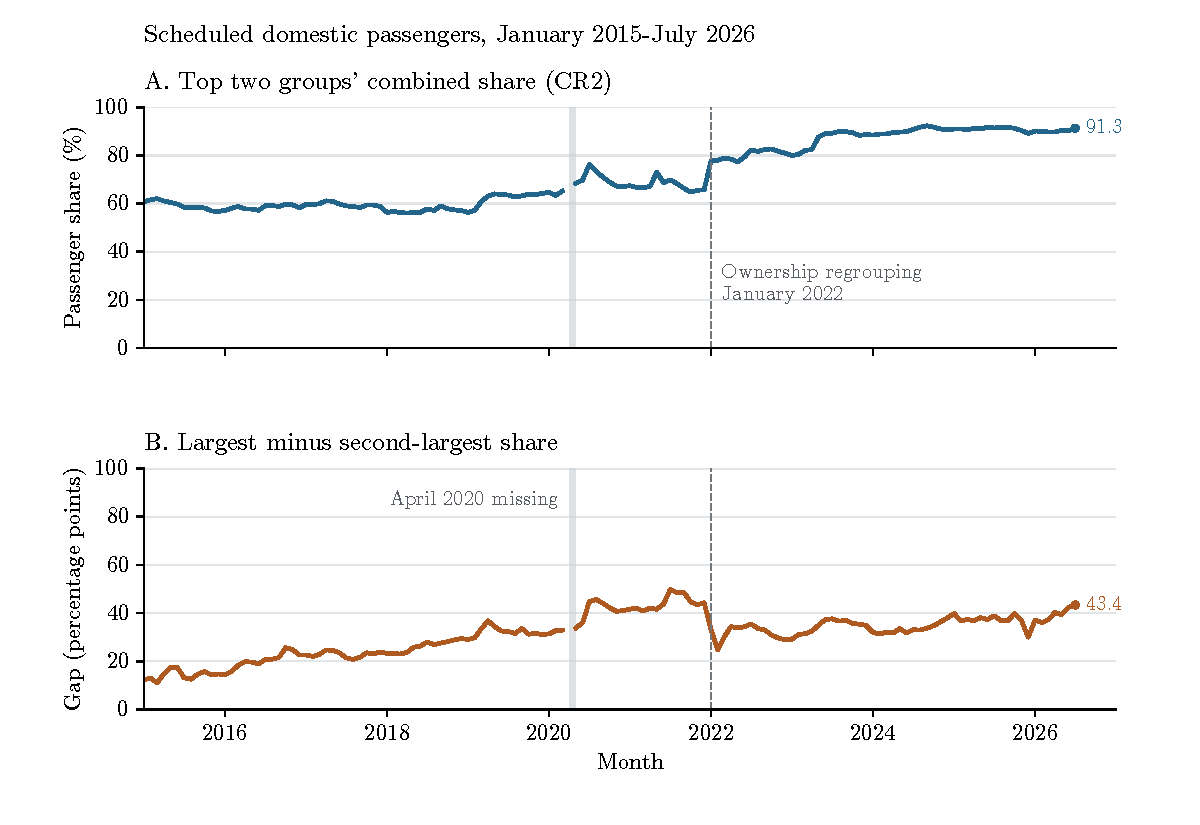
\includegraphics[width=\linewidth]{figures/o4_national_cr2_share_gap.pdf}
\caption{National concentration and share asymmetry, 2015--2026.}
\label{fig:o4-national-eda}
\vspace{2pt}
\begin{minipage}{\linewidth}
\footnotesize\setstretch{1.1}
\textit{Source:} DGCA monthly traffic via \href{https://github.com/mkubicek/india-aviation-stats/tree/16770ac59dae61ce7b80fd8bd67dd7f4cef280a6}{Kubicek (2026)}; authors' calculations.
\end{minipage}
\end{figure}
\end{mergedcontribution}
\begin{mergedcontribution}{authorMeena}
\textbf{Exits: exploratory analysis.} Neither exit was sudden (Figure~\ref{fig:o2-exits}). Jet Airways' passenger share fell from 16.2\% to 5.7\% in the year before its April 2019 exit, and Go First's from 11.1\% to 6.4\% in the year before its May 2023 exit, as both grounded aircraft. Some traffic therefore moved before the exit month, so the before-window already includes part of the shift and the before-and-after comparison may understate it. IndiGo rose most around both exits, from about 43\% to 48\% after Jet Airways and from about 57\% to 62\% after Go First. Section~\ref{sec:o2-results} uses these before-and-after windows to measure how much of each exiting airline's share every group absorbed.

\begin{figure}[H]
\centering
\color{authorMeena}
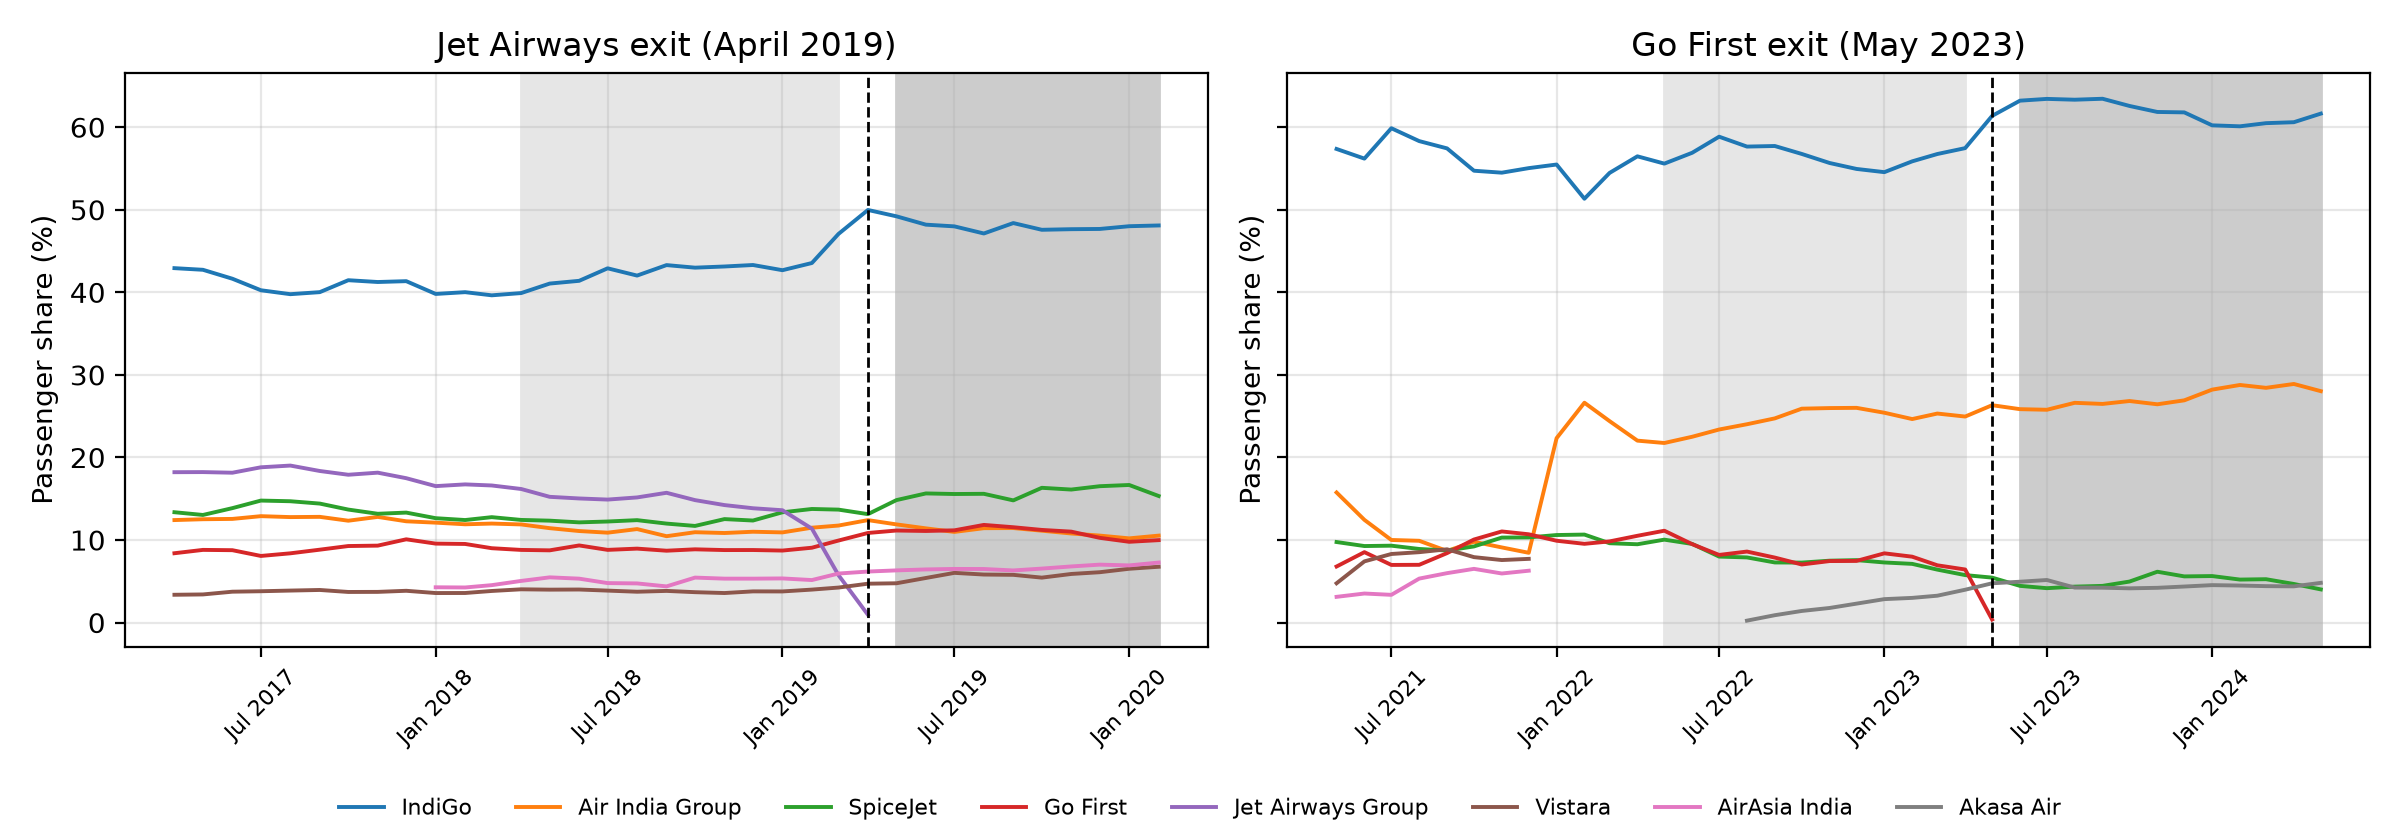
\includegraphics[width=\textwidth]{o2_exit_share_paths.png}
\caption{Monthly passenger shares by ownership group around the Jet Airways and Go First exits}\label{fig:o2-exits}
\sourcenote{DGCA monthly airline statistics via \textcite{kubicek2026aviationstats}; authors' calculations. Light shading: 12-month pre-exit window; dark shading: post-exit window (10 months for Jet Airways, ending before COVID-19); dashed line: exit month, excluded from both windows. The Air India Group's jump in January 2022 is the Tata acquisition grouping, not an exit effect.}
\end{figure}

\textbf{Tata consolidation: descriptive analysis.} The brands brought under one owner in January 2022 held 22.5\% of passengers, and those merged in late 2024 held 29.3\% (Table~\ref{tab:o2-tata}). These shares are the inputs to the mechanical \HHI{} calculation in Section~\ref{sec:o2-results}.

\begin{table}[H]
\centering
\color{authorMeena}
\caption{Passenger shares of the Tata brands before each consolidation step (\%)}\label{tab:o2-tata}
\small
\fontsize{10}{12}\selectfont\setstretch{1}\setlength{\tabcolsep}{3pt}
\renewcommand{\arraystretch}{1.15}
\begin{tabular}{|>{\raggedright\arraybackslash}p{\dimexpr0.32\linewidth-2\tabcolsep-1.1666666666666667\arrayrulewidth\relax}|>{\raggedright\arraybackslash}p{\dimexpr0.13\linewidth-2\tabcolsep-1.1666666666666667\arrayrulewidth\relax}|>{\raggedright\arraybackslash}p{\dimexpr0.14\linewidth-2\tabcolsep-1.1666666666666667\arrayrulewidth\relax}|>{\raggedright\arraybackslash}p{\dimexpr0.12\linewidth-2\tabcolsep-1.1666666666666667\arrayrulewidth\relax}|>{\raggedright\arraybackslash}p{\dimexpr0.18\linewidth-2\tabcolsep-1.1666666666666667\arrayrulewidth\relax}|>{\raggedright\arraybackslash}p{\dimexpr0.11\linewidth-2\tabcolsep-1.1666666666666667\arrayrulewidth\relax}|}
\hline
\textbf{Step (shares in)} & \textbf{Air India} & \textbf{AI Express} & \textbf{Vistara} & \textbf{AirAsia India\textsuperscript{a}} & \textbf{Total} \\
\hline
Acquisition, Jan 2022 (Dec 2021) & 8.39 & 0.07 & 7.72 & 6.28 & 22.46 \\
\hline
Mergers, Dec 2024 (Sep 2024) & 11.14 & 3.97 & 10.04 & 4.11 & 29.26 \\
\hline
\end{tabular}
\sourcenote{DGCA monthly airline statistics via \textcite{kubicek2026aviationstats}; authors' calculations. \textsuperscript{a}Renamed AIX Connect. September 2024 is the last month before the AIX Connect merger (October 2024) and the Vistara merger (November 2024).}
\end{table}
\end{mergedcontribution}

\FloatBarrier
\subsubsection{Entrant traffic patterns}
\begin{mergedcontribution}{authorSweta}
Figure~\ref{fig:o3-life} shows the first and last months with recorded passenger traffic and the peak national share of each of the nine entrants. For airlines still operating, the bars end at the July 2026 data cutoff. Event-time comparisons and the assessment of meaningful and persistent entry follow in Section~\ref{sec:review-o3-results}.

\begin{minipage}{\textwidth}
\centering
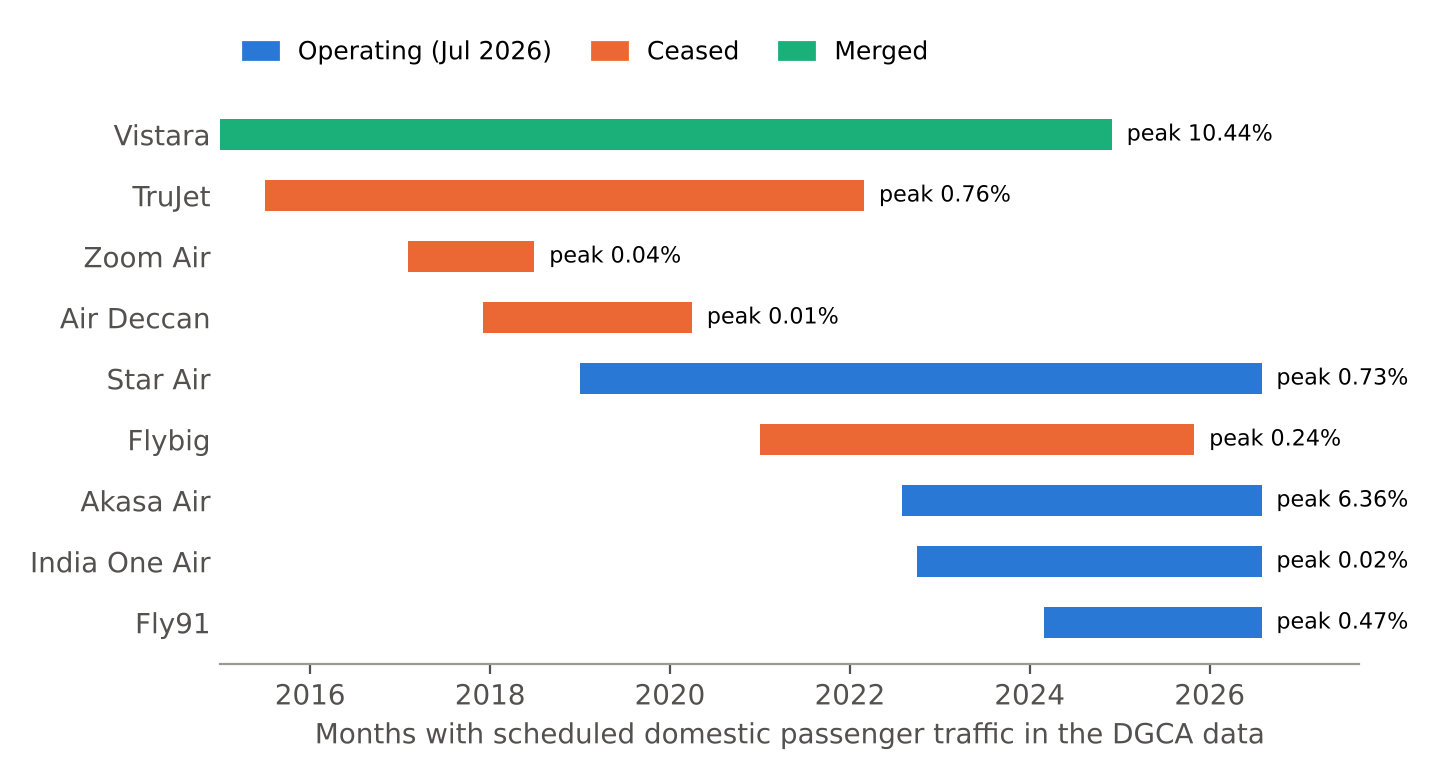
\includegraphics[width=0.92\textwidth]{figures/fig_o3_lifespans.png}
\captionof{figure}{O3: Operating span and peak passenger share of the nine entrants, January 2015--July 2026; colour shows the outcome at July 2026. Source: DGCA via Kubicek (2026); authors' calculations.}
\label{fig:o3-life}
\end{minipage}
\end{mergedcontribution}

\FloatBarrier
\subsubsection{Capacity and passenger traffic}
ASK and RPK provide the inputs for comparing offered capacity and passenger traffic. The event windows below are used for exit comparisons, while the two December observations supply the capacity-buffer analysis. These are different comparisons from the same national dataset.
\begin{mergedcontribution}{authorMeena}
The market grew in both post-exit windows, with passengers rising faster than seat-km, so rivals mainly filled existing seats (Table~\ref{tab:o2-market}).

\begin{table}[H]
\centering
\color{authorMeena}
\caption{Market size and capacity before and after each exit (monthly averages)}\label{tab:o2-market}
\small
\setlength{\tabcolsep}{5pt}
\fontsize{10}{12}\selectfont\setstretch{1}\setlength{\tabcolsep}{3pt}
\renewcommand{\arraystretch}{1.15}
\begin{tabular}{|>{\raggedright\arraybackslash}p{\dimexpr0.12\linewidth-2\tabcolsep-1.1666666666666667\arrayrulewidth\relax}|>{\raggedright\arraybackslash}p{\dimexpr0.24\linewidth-2\tabcolsep-1.1666666666666667\arrayrulewidth\relax}|>{\raggedright\arraybackslash}p{\dimexpr0.16\linewidth-2\tabcolsep-1.1666666666666667\arrayrulewidth\relax}|>{\raggedright\arraybackslash}p{\dimexpr0.17\linewidth-2\tabcolsep-1.1666666666666667\arrayrulewidth\relax}|>{\raggedright\arraybackslash}p{\dimexpr0.13\linewidth-2\tabcolsep-1.1666666666666667\arrayrulewidth\relax}|>{\raggedright\arraybackslash}p{\dimexpr0.18\linewidth-2\tabcolsep-1.1666666666666667\arrayrulewidth\relax}|}
\hline
\textbf{Exit} & \textbf{Window} & \textbf{Passengers (million)} & \textbf{Capacity (billion seat-km)} & \textbf{Load factor (\%)} & \textbf{Average no. of groups with $\geq$1\% share} \\
\hline
Jet Airways & Apr 2018--Mar 2019 & 11.69 & 13.07 & 86.0 & 8.0 \\
\hline
 & May 2019--Feb 2020 & 12.25 & 13.60 & 87.1 & 7.0 \\
\hline
Go First & May 2022--Apr 2023 & 11.53 & 13.29 & 84.1 & 5.6 \\
\hline
 & Jun 2023--May 2024 & 12.88 & 14.25 & 87.2 & 4.6 \\
\hline
\end{tabular}
\sourcenote{DGCA monthly airline statistics via \textcite{kubicek2026aviationstats}; authors' calculations. Capacity (seat-km) $=$ seats offered $\times$ kilometres flown. Load factor $= 100 \times \dfrac{\text{passenger-km}}{\text{seat-km}}$, the share of seats filled.}
\end{table}
\end{mergedcontribution}
\begin{mergedcontribution}{authorGoutham}
The same national dataset provides the capacity inputs. Between December 2024 and December 2025, rivals' offered capacity rises from 6.385 to 6.619 billion seat-kilometres, while passenger traffic rises from 5.493 to 5.947 billion passenger-kilometres. Table~\ref{tab:o4-capacity-inputs} gives the complete inputs.

\begin{minipage}{\linewidth}
\captionsetup{font=small,labelfont=bf,justification=raggedright,singlelinecheck=false,hypcap=false}
\captionof{table}{Capacity and passenger-traffic inputs for the December comparison.}
\label{tab:o4-capacity-inputs}
\centering
{\small\setstretch{1.1}\fontsize{10}{12}\selectfont\setstretch{1}\setlength{\tabcolsep}{3pt}
\renewcommand{\arraystretch}{1.15}
\begin{tabular}{|>{\raggedright\arraybackslash}p{\dimexpr0.17\linewidth-2\tabcolsep-1.25\arrayrulewidth\relax}|>{\raggedright\arraybackslash}p{\dimexpr0.21\linewidth-2\tabcolsep-1.25\arrayrulewidth\relax}|>{\raggedright\arraybackslash}p{\dimexpr0.31\linewidth-2\tabcolsep-1.25\arrayrulewidth\relax}|>{\raggedright\arraybackslash}p{\dimexpr0.31\linewidth-2\tabcolsep-1.25\arrayrulewidth\relax}|}
\hline
\textbf{Month} & \textbf{Airlines} & \textbf{Offered capacity (billion seat-km)} & \textbf{Passenger traffic (billion passenger-km)} \\
\hline
Dec 2024 & IndiGo & 10.053 & 9.113 \\
\hline
Dec 2024 & Other airlines & 6.385 & 5.493 \\
\hline
Dec 2025 & IndiGo & 9.312 & 8.208 \\
\hline
Dec 2025 & Other airlines & 6.619 & 5.947 \\
\hline
\end{tabular}
\par}
\vspace{4pt}
{\footnotesize\setstretch{1.1}\raggedright\textit{Source:} DGCA monthly airline traffic via \href{https://github.com/mkubicek/india-aviation-stats/tree/16770ac59dae61ce7b80fd8bd67dd7f4cef280a6}{Kubicek (2026)}; authors' calculations.\par}
\end{minipage}
\end{mergedcontribution}

\FloatBarrier
\subsection{DGCA approved flight schedules}
\label{sec:o4-route-data}
\subsubsection{Coverage and samples}
The route evidence uses recovered DGCA schedules, pooling both directions of each airport pair. The entrant analysis retains airline brands and uses seasonal snapshots alongside monthly records. The concentration analysis combines brands by ownership and follows a fixed top-20 sample. Table~\ref{tab:review-route-samples} distinguishes these samples rather than adding their counts together.
\begin{resultstable}{Samples drawn from the DGCA schedule archive.}{tab:review-route-samples}
\color{black}
\begin{tabular}{|>{\raggedright\arraybackslash}p{\dimexpr0.28\linewidth-2\tabcolsep-1.3333333333333333\arrayrulewidth\relax}|>{\raggedright\arraybackslash}p{\dimexpr0.38\linewidth-2\tabcolsep-1.3333333333333333\arrayrulewidth\relax}|>{\raggedright\arraybackslash}p{\dimexpr0.34\linewidth-2\tabcolsep-1.3333333333333333\arrayrulewidth\relax}|}
\hline
\textbf{Sample} & \textbf{Coverage} & \textbf{Observation} \\
\hline
Entrant seasonal snapshots & Nine entrants, 225 entrant--airport-pair observations & Weekly departures on the selected mid-season date \\
\hline
Entrant major-route series & 20 airport pairs, April 2019--July 2026 & Airline and airport pair in one month \\
\hline
TruJet regional extension & 30 airport pairs across 14 observed months in 2019--2022 & Airline and airport pair in one month \\
\hline
Ownership-group concentration panel & 20 fixed airport pairs, 1,150 retained observations across 66 available months, April 2019--September 2026 & Airport pair in one month \\
\hline
\end{tabular}
\par\vspace{5pt}{\footnotesize\setstretch{1.05}\raggedright \textbf{Note:} The seasonal snapshots use 15 January or 15 July. The top-20 sample is selected using 2025 passenger totals, with a top-ten subset. The samples overlap and have different units.\par\textbf{Source:} Sweta\textquotesingle s and Goutham\textquotesingle s DGCA schedule preparation and source descriptions.\par}
\end{resultstable}

\subsubsection{Scheduled-flight shares and concentration}
Brand shares describe an entrant's scheduled presence on an airport pair. Ownership-group shares describe concentration after combining commonly owned brands. The concentration figures below use ownership-group shares. Entrant route positions are reported in Section~\ref{sec:review-o3-results}.
\begin{mergedcontribution}{authorGoutham}
Coverage ranges from 12 to 20 airport pairs per observed month. Median HHI is 3,711, with the middle half between 3,180 and 4,244 (Figure~\ref{fig:o4-route-eda}). These measures use ownership groups' scheduled-flight shares. Gaps indicate unavailable data.

\begin{figure}[H]
\centering
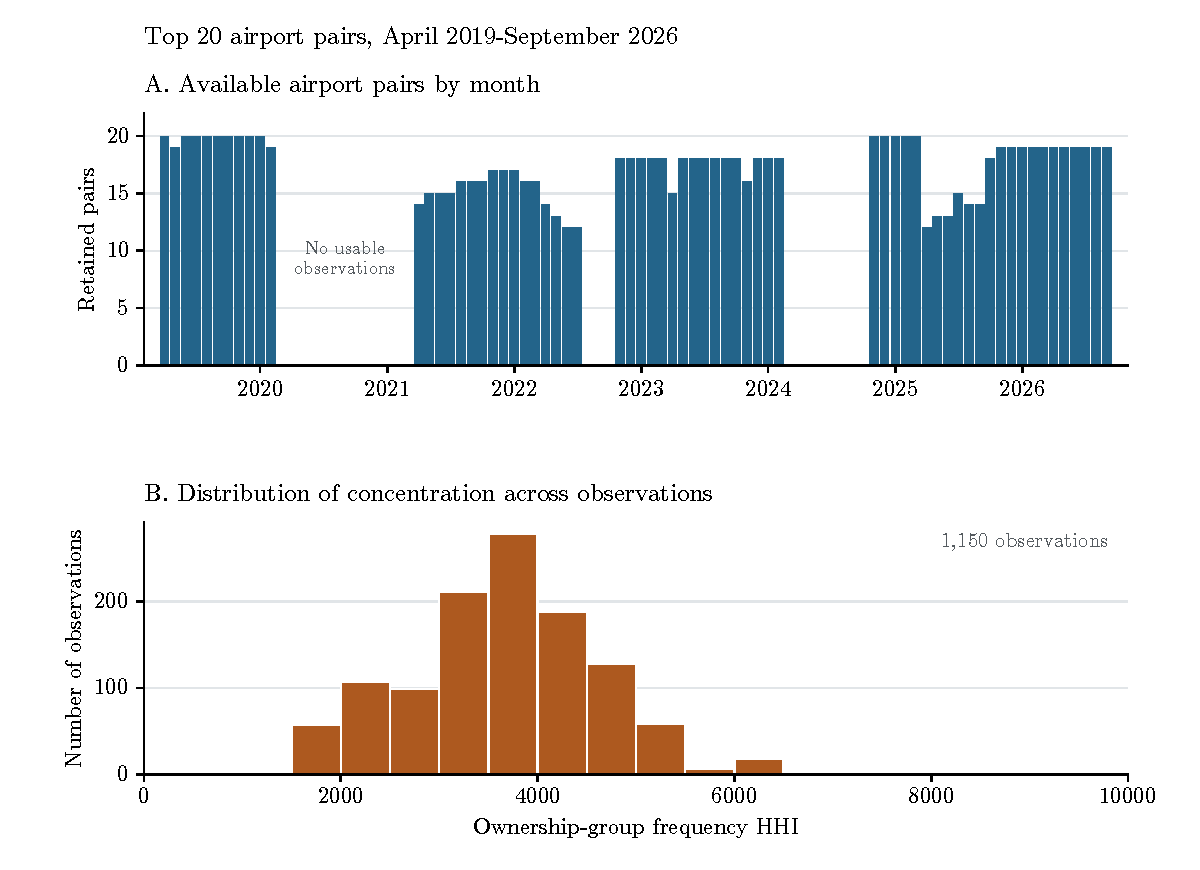
\includegraphics[width=\linewidth]{figures/o4_route_coverage_hhi.pdf}
\caption{Route-data coverage and the distribution of ownership-group frequency HHI.}
\label{fig:o4-route-eda}
\vspace{2pt}
\begin{minipage}{\linewidth}
\footnotesize\setstretch{1.1}
\textit{Source:} DGCA approved domestic schedules; authors' calculations.
\end{minipage}
\end{figure}

Figure~\ref{fig:o4-route-heatmap} shows how HHI varies across individual airport pairs over time. Each row represents one airport pair and each column one calendar month. Colours use a common 0--10,000 HHI scale. Grey cells indicate unavailable data, and gaps are not interpolated.

\begin{figure}[H]
\centering
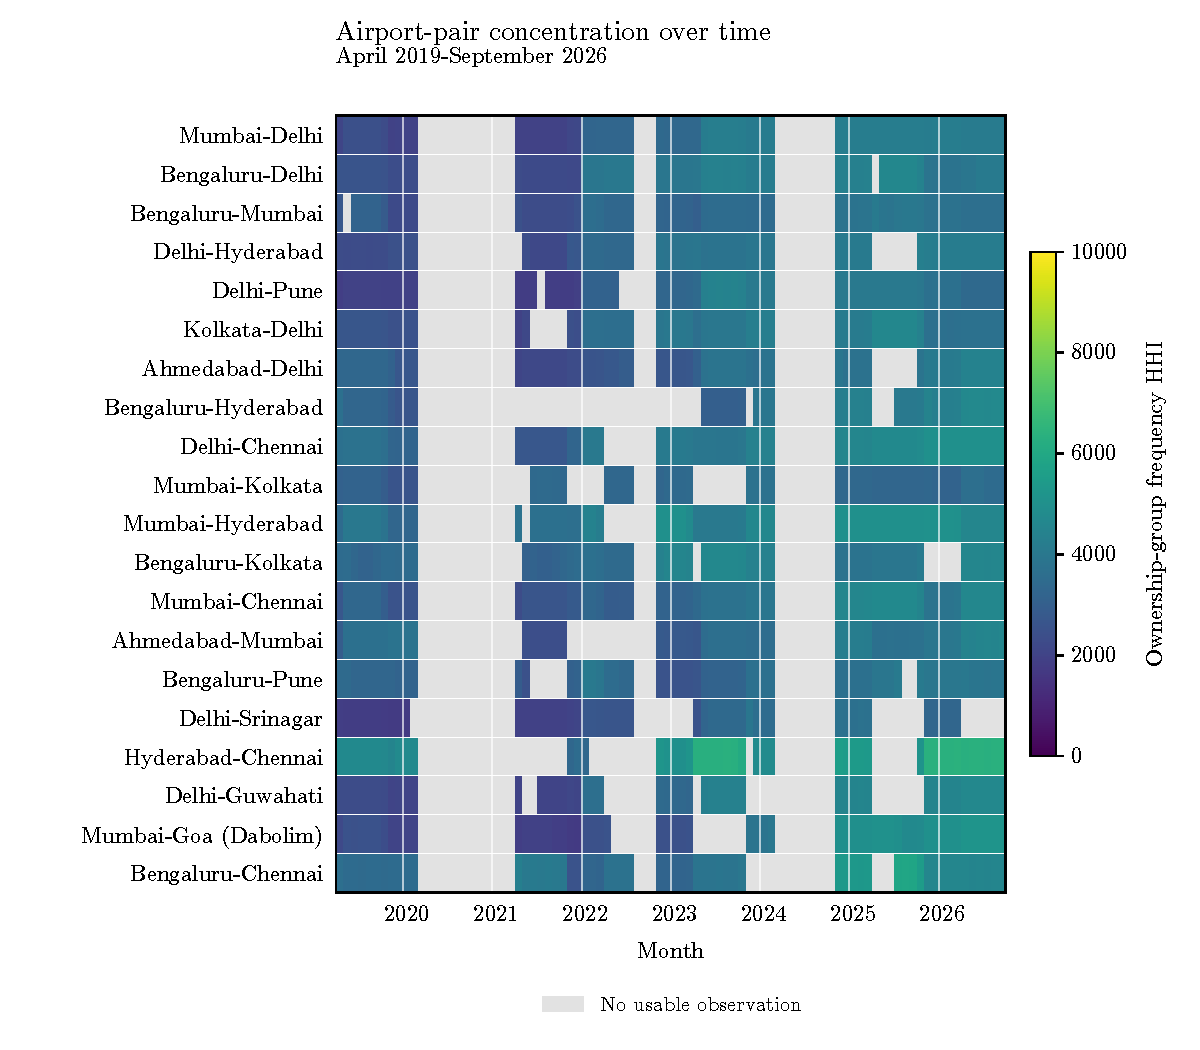
\includegraphics[width=\linewidth]{figures/o4_route_hhi_heatmap.pdf}
\caption{Ownership-group frequency HHI by airport pair and month.}
\label{fig:o4-route-heatmap}
\vspace{2pt}
\begin{minipage}{\linewidth}
\footnotesize\setstretch{1.1}
\textit{Source:} DGCA approved domestic schedules; authors' calculations.
\end{minipage}
\end{figure}
\end{mergedcontribution}

\FloatBarrier
\clearpage
\subsection{Company financial and regulatory records}
The financial evidence comes from company and rating reports, parliamentary replies and selected press reports. Coverage differs across airlines and years, and net results are kept separate from operating results. Table~\ref{tab:review-financial-coverage} describes the available inputs. Financial comparisons and calculated margins are assigned to Section~\ref{sec:review-o3-results}.
\begin{mergedcontribution}{authorSweta}
\begin{resultstable}{Financial and funding records used in O3.}{tab:review-financial-coverage}
\color{authorSweta}
\begin{tabular}{|>{\raggedright\arraybackslash}p{\dimexpr0.27\linewidth-2\tabcolsep-1.3333333333333333\arrayrulewidth\relax}|>{\raggedright\arraybackslash}p{\dimexpr0.36\linewidth-2\tabcolsep-1.3333333333333333\arrayrulewidth\relax}|>{\raggedright\arraybackslash}p{\dimexpr0.37\linewidth-2\tabcolsep-1.3333333333333333\arrayrulewidth\relax}|}
\hline
\textbf{Source} & \textbf{Coverage} & \textbf{Available inputs} \\
\hline
ICRA rating reports & Vistara: FY2023--FY2024. Akasa Air: FY2025--FY2026. & Operating income, profit after tax and funding evidence \\
\hline
Lok Sabha reply, December 2025 & Available entrant records for FY2023--FY2025 & Reported profit or loss after tax, with provisional figures identified \\
\hline
DGCA operating results reported in Parliament & Available airline-year records for FY2017--FY2021 & Revenue and operating results, with revisions and provisional figures identified \\
\hline
Company releases and selected press reports & Airline-specific dates and financial years & Funding announcements, operating outcomes and additional revenue figures \\
\hline
\end{tabular}
\par\vspace{5pt}{\footnotesize\setstretch{1.05}\raggedright \textbf{Note:} These records do not form a balanced annual panel. Unavailable values are not zero, and different accounting bases are not pooled.\par\textbf{Source:} ICRA (2024, 2026), Ministry of Civil Aviation (2025), Rajya Sabha (2019, 2021), and the company/press records listed with the O3 references.\par}
\end{resultstable}
\end{mergedcontribution}

\clearpage
\section{Analysis and Results}
\subsection{O1: Concentration changes and ownership effects}
\label{sec:review-o1-results}
\begin{mergedcontribution}{authorSowmya}
\subsubsection{O1: Index over months and drift points}
 Figure~\ref{fig:o1-its} plots observed and fitted HHI against the 5,000 symmetric-duopoly reference, CR2, and the concealed wedge, with events T1--T4 and drift points D1--D7. Ownership-HHI rises as a staircase, with steps of $+312$, $+900$, $+640$ and $+137$ points and no plateau revisited. The series coincide at the two exits (share shifts) and separate at T2 (regrouping), when Brand-HHI falls 300--600 points below the others. CR2 steps by $+5.7$, $+17.9$, $+9.3$ and $+1.4$ points. The wedge peaks near 600 points in late 2024.

\begin{minipage}{\linewidth}
\centering
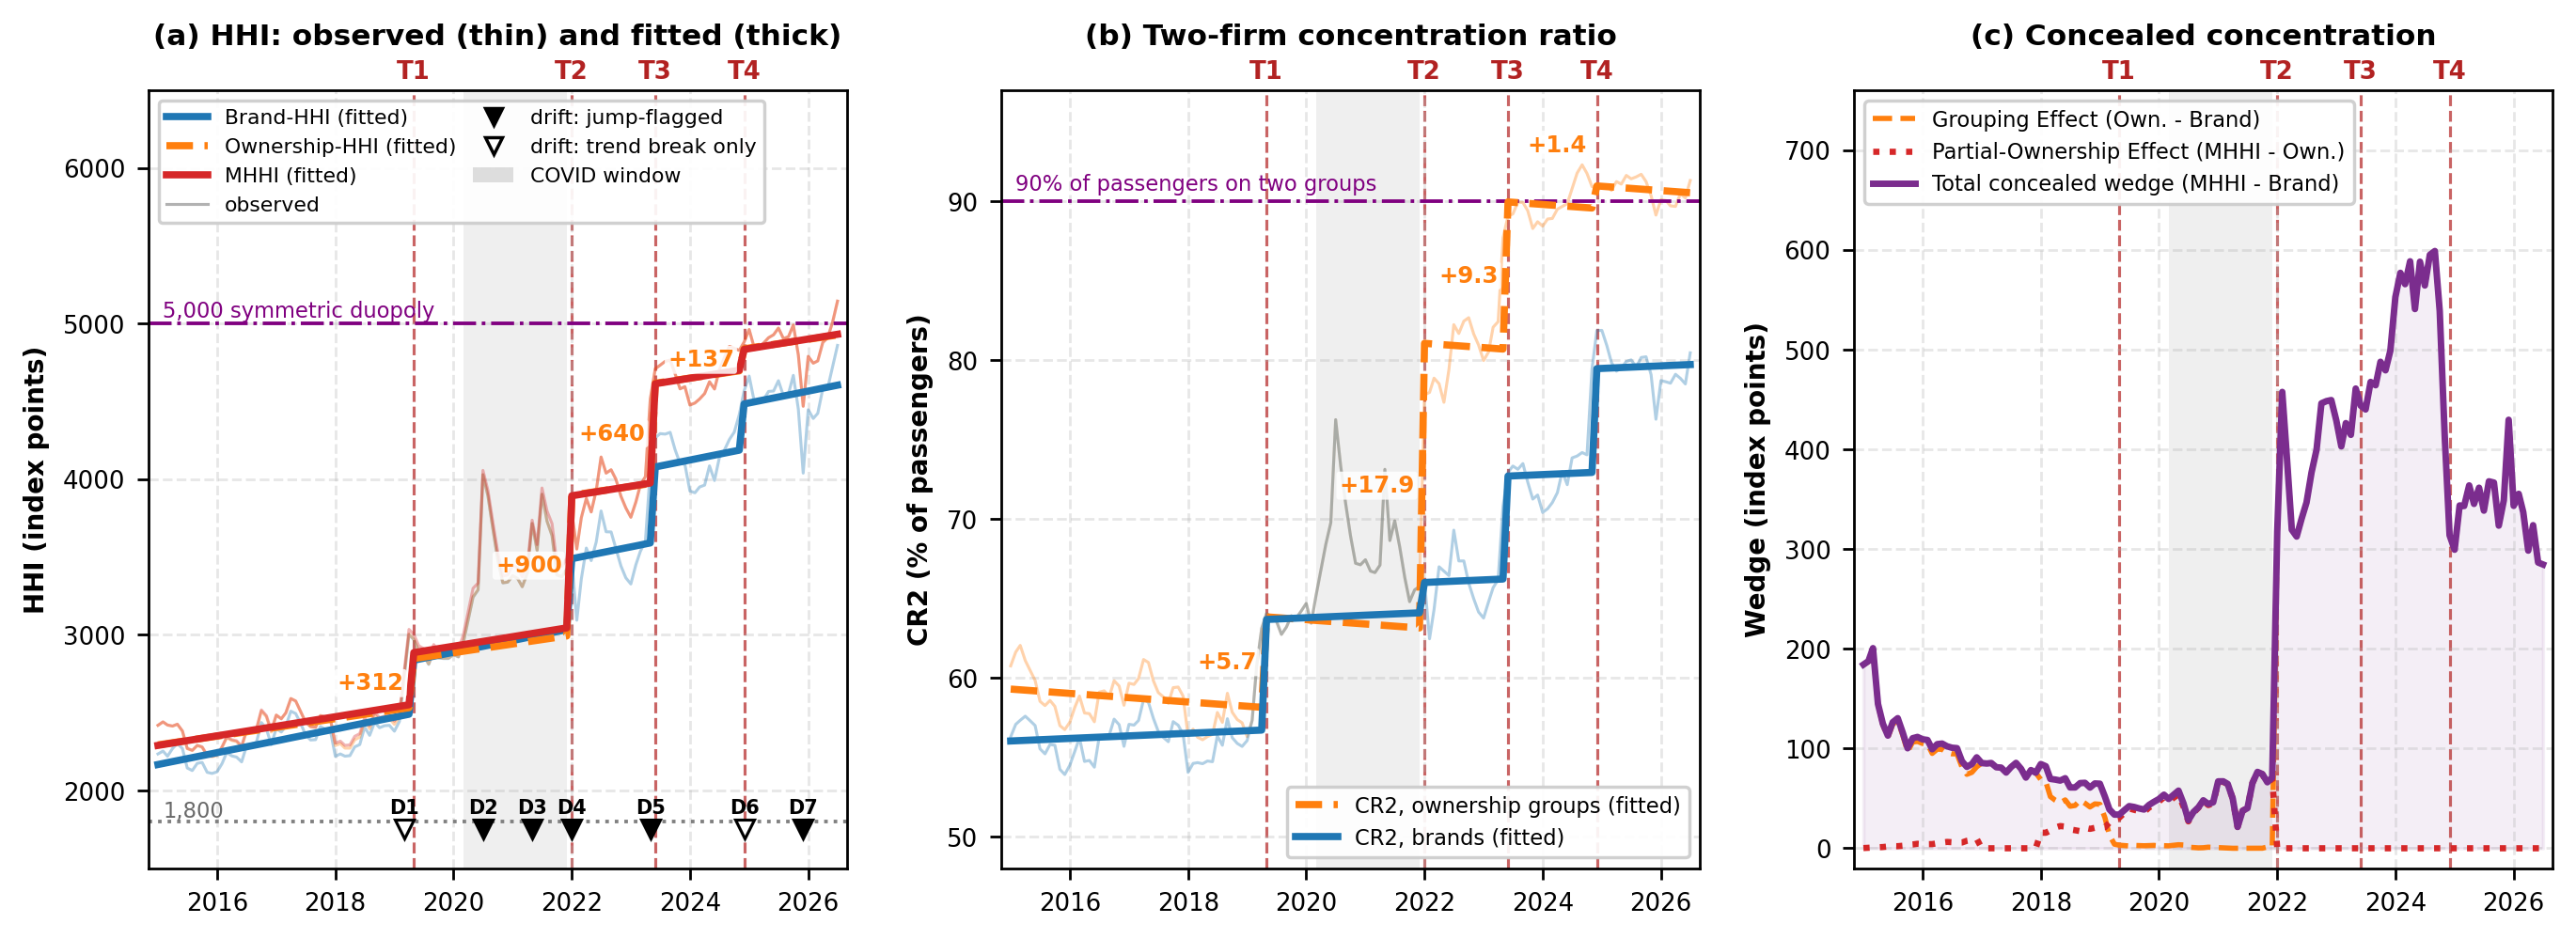
\includegraphics[width=\linewidth]{figures/o1_hhi.png}
\captionof{figure}{O1: Interrupted time-series view of national concentration, January 2015--July 2026.}
\label{fig:o1-its}
\vspace{2pt}
\par\footnotesize\setstretch{1.1}
\textit{Note:} (a) Brand-, Ownership- and MHHI: observed (thin) and fitted (thick) values from Equation~O1.2, keeping the trend and the four event steps, with COVID and month-of-year terms netted out; figures beside each step are Ownership-HHI steps in points. (b) CR2 with its steps in percentage points. (c) Grouping Effect, Partial-Ownership Effect and their sum, the total concealed wedge. T1--T4: Jet exit, Tata acquisition, Go First exit, legal mergers. D1--D7: drift points (filled markers flagged by the jump detector). Grey band: COVID window.\par
\textit{Source:} DGCA monthly traffic via \href{https://github.com/mkubicek/india-aviation-stats/tree/16770ac59dae61ce7b80fd8bd67dd7f4cef280a6}{Kubicek (2026)}; authors' calculations.
\end{minipage}

Table~\ref{tab:o1-drift} gives, for each drift point, the index change and the reason for the shift in level.

\begin{minipage}{\linewidth}
\captionsetup{font={small,color=authorSowmya},labelfont=bf,justification=raggedright,singlelinecheck=false,hypcap=false}
\captionof{table}{O1: Drift points and the reason for each level shift.}
\label{tab:o1-drift}
\centering
{\footnotesize\setstretch{1.0}\setlength{\tabcolsep}{3pt}
\fontsize{9}{10.8}\selectfont\setstretch{1}\setlength{\tabcolsep}{3pt}
\renewcommand{\arraystretch}{1.15}
\begin{tabular}{|>{\raggedright\arraybackslash}p{\dimexpr0.045\linewidth-2\tabcolsep-1.125\arrayrulewidth\relax}|>{\raggedright\arraybackslash}p{\dimexpr0.12\linewidth-2\tabcolsep-1.125\arrayrulewidth\relax}|>{\raggedright\arraybackslash}p{\dimexpr0.09\linewidth-2\tabcolsep-1.125\arrayrulewidth\relax}|>{\raggedright\arraybackslash}p{\dimexpr0.09\linewidth-2\tabcolsep-1.125\arrayrulewidth\relax}|>{\raggedright\arraybackslash}p{\dimexpr0.09\linewidth-2\tabcolsep-1.125\arrayrulewidth\relax}|>{\raggedright\arraybackslash}p{\dimexpr0.19\linewidth-2\tabcolsep-1.125\arrayrulewidth\relax}|>{\raggedright\arraybackslash}p{\dimexpr0.13\linewidth-2\tabcolsep-1.125\arrayrulewidth\relax}|>{\raggedright\arraybackslash}p{\dimexpr0.245\linewidth-2\tabcolsep-1.125\arrayrulewidth\relax}|}
\hline
\textbf{ID} & \textbf{Window} & \textbf{$\Delta$Br.} & \textbf{$\Delta$Own.} & \textbf{$\Delta$CR2} & \textbf{Largest share movers (pp)} & \textbf{Type} & \textbf{Reason for the shift} \\
\hline
D1 & Feb--Apr 2019 & $+558$ & $+531$ & $+5.8$ & Jet group $-10.4$; IndiGo $+6.4$ & Share shift; permanent & Jet Airways exit; IndiGo took most of its passengers \\
\hline
D2 & Jun--Jul 2020 & $+741$ & $+739$ & $+6.5$ & IndiGo $+7.6$; Air India Group $-3.3$ & Share shift; retraced by Nov 2020 & Post-lockdown restart; IndiGo regained volume first \\
\hline
D3 & Apr--May 2021 & $+321$ & $+321$ & $+6.0$ & Air India Group $+6.1$; AirAsia India $-3.2$ & Share shift; retraced by Oct 2021 & Second COVID wave \\
\hline
D4 & Dec 2021--Jan 2022 & $+51$ & $+367$ & $+12.1$ & Air India Group $+13.9$ (Vistara $-7.7$, AirAsia India $-6.3$) & Regrouping; Own.\ and MHHI only & Tata grouping: Vistara and AirAsia India reported inside Air India \\
\hline
D5 & Apr--Jun 2023 & $+664$ & $+693$ & $+6.6$ & Go First $-6.4$; IndiGo $+5.7$ & Share shift; permanent & Go First exit; IndiGo took most of its passengers \\
\hline
D6 & Nov--Dec 2024 & $+153$ & $+54$ & $0.0$ & Vistara, AIX Connect folded into Air India, Air India Express & Regrouping; Brand only & Legal mergers; fewer reported brands, no share change \\
\hline
D7 & Nov--Dec 2025 & $-411$ & $-330$ & $-1.2$ & IndiGo $-4.0$; Air India Group $+2.8$ & Share shift; reversed Jan 2026 & IndiGo operational disruption \parencite{moca2026indigo} \\
\hline
\end{tabular}\par}
\vspace{4pt}
{\footnotesize\setstretch{1.0}\raggedright\textit{Note:} Changes are index points between the months shown; $\Delta$CR2 is in percentage points on ownership groups. A flagged May 2020 change spans two months because April 2020 is missing. Reasons are the events coinciding with each drift, not causal estimates.\par
\textit{Source:} DGCA monthly airline traffic via \href{https://github.com/mkubicek/india-aviation-stats/tree/16770ac59dae61ce7b80fd8bd67dd7f4cef280a6}{Kubicek (2026)}; authors' calculations.\par}
\end{minipage}

The two exits (D1, D5) raise all indices alike and never reverse; Jet's group share was zero by May 2019, so its drift starts in March. The reclassifications (D4, D6) move only the indices that depend on grouping or reporting. The transient drifts (D2, D3, D7) reverse within months; D2 ($M=8.3$--9.1) is 94\% reversed by November 2020.

\subsubsection{O1: Event steps in concentration}
All four event steps are positive and significant in every model (Table~\ref{tab:o1-regression}). The Tata acquisition (900 vs.\ 449 points) and the Go First exit (640 vs.\ 482) are larger once brands are grouped by owner; the mergers are smaller (137 vs.\ 291) because they combined brands already grouped. The steps sum to 1,988 points for Ownership-HHI against 1,563 for Brand-HHI, so brand-level counting misses about a fifth of the event-driven rise. MHHI's Tata step is 56 points smaller than Ownership-HHI's because the partial-ownership wedge ends there. Re-dating the Jet and Go First steps to their drift months (March 2019, May 2023) lifts the Ownership-HHI sum to 2,211 and $R^2$ from 0.981 to 0.985 without changing the ranking.

\begin{minipage}{\linewidth}
\captionsetup{font={small,color=authorSowmya},labelfont=bf,justification=raggedright,singlelinecheck=false,hypcap=false}
\captionof{table}{O1: Segmented regression of monthly concentration indices (Equation~O1.2).}
\label{tab:o1-regression}
\centering
{\small\setstretch{1.1}\setlength{\tabcolsep}{5pt}
\fontsize{10}{12}\selectfont\setstretch{1}\setlength{\tabcolsep}{3pt}
\renewcommand{\arraystretch}{1.15}
\begin{tabular}{|>{\raggedright\arraybackslash}p{\dimexpr0.34\linewidth-2\tabcolsep-1.25\arrayrulewidth\relax}|>{\raggedright\arraybackslash}p{\dimexpr0.22\linewidth-2\tabcolsep-1.25\arrayrulewidth\relax}|>{\raggedright\arraybackslash}p{\dimexpr0.22\linewidth-2\tabcolsep-1.25\arrayrulewidth\relax}|>{\raggedright\arraybackslash}p{\dimexpr0.22\linewidth-2\tabcolsep-1.25\arrayrulewidth\relax}|}
\hline
\textbf{Regressor} & \textbf{Brand HHI} & \textbf{Ownership HHI} & \textbf{MHHI} \\
\hline
Time trend (points per month) & 6.34\textsuperscript{**} (1.94) & 4.68\textsuperscript{*} (2.00) & 5.12\textsuperscript{*} (2.01) \\
\hline
Post-Jet exit (May 2019) & 340.83\textsuperscript{**} (78.99) & 311.51\textsuperscript{**} (79.12) & 330.33\textsuperscript{**} (79.50) \\
\hline
Post-Tata acquisition (Jan 2022) & 449.31\textsuperscript{**} (78.08) & 899.79\textsuperscript{**} (82.94) & 843.69\textsuperscript{**} (82.94) \\
\hline
Post-Go First exit (Jun 2023) & 481.99\textsuperscript{**} (50.45) & 640.03\textsuperscript{**} (56.18) & 632.96\textsuperscript{**} (55.21) \\
\hline
Post-legal mergers (Dec 2024) & 290.97\textsuperscript{**} (73.85) & 137.13\textsuperscript{*} (54.72) & 128.51\textsuperscript{*} (55.59) \\
\hline
COVID (Mar 2020--Dec 2021) & 517.84\textsuperscript{**} (44.59) & 543.41\textsuperscript{**} (45.53) & 547.56\textsuperscript{**} (45.25) \\
\hline
Sum of the four steps & 1{,}563 (222) & 1{,}988 (222) & 1{,}935 (223) \\
\hline
$R^2$ & 0.972 & 0.981 & 0.981 \\
\hline
Durbin--Watson & 0.92 & 0.93 & 0.94 \\
\hline
\end{tabular}\par}
\vspace{4pt}
{\footnotesize\setstretch{1.1}\raggedright\textit{Note:} Newey--West standard errors (12 lags) in parentheses; $n=138$. \textsuperscript{*}$p<0.05$, \textsuperscript{**}$p<0.01$. Constant and eleven month-of-year dummies included. Breusch--Godfrey (12 lags) rejects no autocorrelation and the ADF test rejects a unit root in the residuals ($p<0.001$ in all three models).\par
\textit{Source:} DGCA monthly airline traffic via \href{https://github.com/mkubicek/india-aviation-stats/tree/16770ac59dae61ce7b80fd8bd67dd7f4cef280a6}{Kubicek (2026)}; authors' calculations.\par}
\end{minipage}

CR2 on ownership groups averages 72.0\%, rising from 58.7\% to 90.7\% across the periods and reaching 91.3\% in July 2026 (IndiGo 67.4\%, Air India Group 24.0\%). Its steps are $+5.7$, $+17.9$, $+9.3$ and $+1.4$ points (total 34.4); at brand level the Tata step is only 1.9 and the merger step 6.5. January 2022 is its largest monthly move ($+12.1$). CR2 and Ownership-HHI correlate at 0.983 in levels but 0.794 in monthly changes (Appendix~\ref{app:o1-cr2}).

\subsubsection{O1: Partial-ownership wedge and grouping gap}
\label{app:o1-wedge}
\textbf{Partial-ownership wedge.} With the stake schedule, the MHHI minus Ownership-HHI wedge exists only before January 2022. Under proportional control it averages 22.9 points (0.8\% of Ownership-HHI) and peaks at 76.6 in September 2021 (2.2\%). It rises with Tata's stake in AirAsia India: about 1.2 points in January--August 2015 (Tata 30\%), 3.8 to March 2016 (41.06\%), 6.7 in April--December 2016 (49\%), 26.2 in 2018--2019, 43.6 in 2020 (51\%) and 58.1 in 2021 (83.67\%). The zero wedge in 2017 is a source gap; interpolating gives 13.5 on average and a pre-2022 mean of 24.9. Treating Tata's 51\% of Vistara as full control raises the pre-2022 mean to 36.9 (maximum 119.6).

\textbf{Grouping gap.} Ownership-HHI is never below Brand-HHI; the gap is under 0.5 points in 10 months (September 2020, February--October 2021) when Air India Express carried almost no scheduled traffic. It steps up by 450 points at the Tata acquisition ($t=17.6$), widens about 5.5 points a month to a peak of 598.7, then falls by 154 points ($t=-5.3$) to 284.5 in July 2026 as Vistara and AIX Connect stop being separate brands. The remaining gap is the Air India--Air India Express split (Table~\ref{tab:o1-gap}).

\begin{minipage}{\linewidth}
\captionsetup{font={small,color=authorSowmya},labelfont=bf,justification=raggedright,singlelinecheck=false,hypcap=false}
\captionof{table}{O1: Grouping gap (Ownership-HHI minus Brand-HHI): period means and regression.}
\label{tab:o1-gap}
\centering
{\small\setstretch{1.1}\setlength{\tabcolsep}{5pt}
\fontsize{10}{12}\selectfont\setstretch{1}\setlength{\tabcolsep}{3pt}
\renewcommand{\arraystretch}{1.15}
\begin{tabular}{|>{\raggedright\arraybackslash}p{\dimexpr0.46\linewidth-2\tabcolsep-1.25\arrayrulewidth\relax}|>{\raggedright\arraybackslash}p{\dimexpr0.18\linewidth-2\tabcolsep-1.25\arrayrulewidth\relax}|>{\raggedright\arraybackslash}p{\dimexpr0.18\linewidth-2\tabcolsep-1.25\arrayrulewidth\relax}|>{\raggedright\arraybackslash}p{\dimexpr0.18\linewidth-2\tabcolsep-1.25\arrayrulewidth\relax}|}
\hline
\textbf{Period} & \textbf{Mean} & \textbf{Min} & \textbf{Max} \\
\hline
Pre-Jet exit & 84.2 & 4.1 & 199.9 \\
\hline
Jet exit to Tata & 1.4 & 0.0 & 3.6 \\
\hline
Tata to mergers & 461.0 & 312.5 & 598.7 \\
\hline
Post mergers & 338.7 & 284.5 & 429.6 \\
\hline
Regression coefficient & Standard model & \multicolumn{2}{r|}{With post-Tata trend} \\
\hline
Post-Tata step & 450.48\textsuperscript{**} (25.58) & \multicolumn{2}{r|}{427.96\textsuperscript{**} (18.97)} \\
\hline
Post-Tata trend (points per month) & -- & \multicolumn{2}{r|}{5.52\textsuperscript{**} (1.95)} \\
\hline
Post-Go First step & 158.05\textsuperscript{**} (38.93) & \multicolumn{2}{r|}{72.18 (40.93)} \\
\hline
Post-legal mergers step & $-153.84$\textsuperscript{**} (28.98) & \multicolumn{2}{r|}{$-247.66$\textsuperscript{**} (38.79)} \\
\hline
$R^2$ & 0.968 & \multicolumn{2}{r|}{0.976} \\
\hline
\end{tabular}\par}
\vspace{4pt}
{\footnotesize\setstretch{1.1}\raggedright\textit{Note:} Values in index points; Newey--West standard errors (12 lags) in parentheses. \textsuperscript{**}$p<0.01$. The Jet exit step is not significant in either model; trend, COVID and month dummies are included.\par}
\end{minipage}
\begin{resultstable}{Partial-ownership adjustment: MHHI minus Ownership-HHI.}{tab:review-o1-wedge}
\color{authorSowmya}
\begin{tabular}{|>{\raggedright\arraybackslash}p{\dimexpr0.44\linewidth-2\tabcolsep-1.3333333333333333\arrayrulewidth\relax}|>{\raggedright\arraybackslash}p{\dimexpr0.25\linewidth-2\tabcolsep-1.3333333333333333\arrayrulewidth\relax}|>{\raggedright\arraybackslash}p{\dimexpr0.31\linewidth-2\tabcolsep-1.3333333333333333\arrayrulewidth\relax}|}
\hline
\textbf{Period} & \textbf{Mean wedge (points)} & \textbf{Maximum wedge (points)} \\
\hline
Before January 2022 & 22.9 & 76.6 (September 2021) \\
\hline
January 2022--July 2026 & 0 & 0 \\
\hline
\end{tabular}
\par\vspace{5pt}{\footnotesize\setstretch{1.05}\raggedright \textbf{Note:} Proportional-control specification. Before January 2022 the reported mean is 0.8\% of Ownership-HHI and the maximum is 2.2\%. AirAsia India\textquotesingle s missing 2017 records produce a zero wedge in that year; the interpolation and alternative-control checks are reported above and in Appendix~\ref{app:o1-stakes}.\par\textbf{Source:} DGCA monthly traffic and the ownership-stake schedule; authors\textquotesingle\ calculations.\par}
\end{resultstable}

\end{mergedcontribution}

\FloatBarrier
\clearpage
\begin{mergedcontribution}{authorMeena}
\subsection{O2: Who gained from exits and consolidation}\label{sec:o2-results}
\textbf{Who absorbed the exits.} IndiGo led passenger-share absorption after both exits: 37.7\% for Jet Airways and 66.0\% for Go First (Table~\ref{tab:o2-absorption}). SpiceJet ranked second after Jet Airways (22.9\%); Akasa Air (35.3\%) and Air India Group (33.7\%) also gained after Go First. Positive absorption exceeds 100\% because SpiceJet and other survivors also lost share; including these losses gives 100\%.

\begin{table}[H]
\centering
\color{authorMeena}
\caption{Share of the exiting airline absorbed by each group, and contribution to the change in \HHI{}}\label{tab:o2-absorption}
\small
\small\setstretch{1}\setlength{\tabcolsep}{5pt}
\renewcommand{\arraystretch}{1.15}
\begin{tabular}{|l|r|r|r|r|r|r|}
\hline
 & \multicolumn{3}{c|}{Jet Airways exit (Apr 2019)} & \multicolumn{3}{c|}{Go First exit (May 2023)} \\
\hline
\textbf{Group} & \textbf{\shortstack{Passengers\\$a_g$ (\%)}} & \textbf{\shortstack{Seat-km\\$a_g$ (\%)}} & \textbf{$c_g$} & \textbf{\shortstack{Passengers\\$a_g$ (\%)}} & \textbf{\shortstack{Seat-km\\$a_g$ (\%)}} & \textbf{$c_g$} \\
\hline
IndiGo & 37.7 & 28.5 & 473 & 66.0 & 66.0 & 632 \\
\hline
SpiceJet & 22.9 & 30.4 & 90 & $-$33.7 & $-$36.2 & $-$34 \\
\hline
Air India Group & $-$1.0 & 1.5 & $-$3 & 33.7 & 30.3 & 141 \\
\hline
Akasa Air & -- & -- & -- & 35.3 & 40.7 & 18 \\
\hline
Go First & 14.1 & 11.4 & 39 & -- & -- & -- \\
\hline
Vistara & 14.3 & 14.2 & 19 & \multicolumn{3}{c|}{in Air India Group} \\
\hline
AirAsia India & 10.6 & 13.3 & 17 & \multicolumn{3}{c|}{in Air India Group} \\
\hline
Others & 1.4 & 0.7 & 0 & $-$1.3 & $-$0.8 & 0 \\
\hline
Exiting airline removed & & & $-$191 & & & $-$65 \\
\hline
Total change in \HHI{} & 100 & 100 & +444 & 100 & 100 & +690 \\
\hline
\end{tabular}
\sourcenote{DGCA monthly airline statistics via \textcite{kubicek2026aviationstats}; authors' calculations. Passengers and Seat-km: absorption $a_g$ (\%), a group's change in mean share divided by the exiting airline's pre-exit mean share. $c_g$: contribution to the change in \HHI{} (points), using passenger shares. Windows: Apr 2018--Mar 2019 vs May 2019--Feb 2020 (Jet Airways); May 2022--Apr 2023 vs Jun 2023--May 2024 (Go First).}
\end{table}

\begin{resultstable}{Capacity-based contributions to the change in concentration after each exit.}{tab:review-o2-capacity-contribution}
\color{authorMeena}
\begin{tabular}{|>{\raggedright\arraybackslash}p{\dimexpr0.38\linewidth-2\tabcolsep-1.3333333333333333\arrayrulewidth\relax}|>{\raggedright\arraybackslash}p{\dimexpr0.32\linewidth-2\tabcolsep-1.3333333333333333\arrayrulewidth\relax}|>{\raggedright\arraybackslash}p{\dimexpr0.3\linewidth-2\tabcolsep-1.3333333333333333\arrayrulewidth\relax}|}
\hline
\textbf{Exit} & \textbf{IndiGo contribution (HHI points)} & \textbf{Total HHI change (points)} \\
\hline
Jet Airways & 352 & 354 \\
\hline
Go First & 599 & 653 \\
\hline
\end{tabular}
\par\vspace{5pt}{\footnotesize\setstretch{1.05}\raggedright \textbf{Note:} Shares use available seat-kilometres. The contribution is IndiGo\textquotesingle s squared average share after the exit minus its squared average share before it. Windows follow Table~\ref{tab:o2-absorption}; the total includes all groups and the exiting airline. Values are rounded.\par\textbf{Source:} DGCA monthly airline statistics; authors\textquotesingle\ capacity-share calculations.\par}
\end{resultstable}


\textbf{Who drove concentration.} IndiGo added 473 \HHI{} points after Jet Airways' exit, exceeding the net rise of 444 because Jet's 191 points disappeared. It added 632 of 690 points (92\%) after Go First. Seat-km results similarly show IndiGo driving both increases.

\textbf{Capacity versus filling seats.} SpiceJet's seat-km absorption exceeded its passenger absorption after Jet Airways (30.4\% versus 22.9\%). Its annual report confirms that it received 74 vacated slots and inducted 31 aircraft made available by Jet's suspension \parencite[p.~62]{spicejet2020annual}. IndiGo showed the reverse pattern, but this alone does not establish fuller seats. Akasa's higher seat-km absorption after Go First partly reflects its ramp-up since August 2022. Go First's engine-related groundings predated its exit \parencite[p.~35]{goair2021drhp}.

\textbf{Tata consolidation.} Ownership \HHI{} rose 373 points in January 2022 against a mechanical 334 from common ownership alone (Table~\ref{tab:o2-mech}); COVID-19 recovery also affects this comparison. At the December 2024 mergers, brand \HHI{} rose 493 points against a mechanical 256. Tata's combined share fell from 28.3\% to 26.7\%, limiting its contribution to about 135 points; IndiGo's growth from 61.5\% to 64.5\% added about 380. Observed increases exceeded mechanical increases at both steps.

\begin{table}[H]
\centering
\color{authorMeena}
\caption{Mechanical and observed change in \HHI{} at each Tata consolidation step (points)}\label{tab:o2-mech}
\small
\fontsize{10}{12}\selectfont\setstretch{1}\setlength{\tabcolsep}{3pt}
\renewcommand{\arraystretch}{1.15}
\begin{tabular}{|>{\raggedright\arraybackslash}p{\dimexpr0.36\linewidth-2\tabcolsep-1.2\arrayrulewidth\relax}|>{\raggedright\arraybackslash}p{\dimexpr0.19\linewidth-2\tabcolsep-1.2\arrayrulewidth\relax}|>{\raggedright\arraybackslash}p{\dimexpr0.15\linewidth-2\tabcolsep-1.2\arrayrulewidth\relax}|>{\raggedright\arraybackslash}p{\dimexpr0.15\linewidth-2\tabcolsep-1.2\arrayrulewidth\relax}|>{\raggedright\arraybackslash}p{\dimexpr0.15\linewidth-2\tabcolsep-1.2\arrayrulewidth\relax}|}
\hline
\textbf{Step} & \textbf{Measure} & \textbf{Mechanical} & \textbf{Observed} & \textbf{Difference} \\
\hline
\raggedright\textbf{Acquisition (Jan 2022)}\newline Tata acquired Air India and Air India Express. & Ownership \HHI{} & +334 & +373 & +39 \\
\hline
\raggedright\textbf{Mergers (Oct--Nov 2024)}\newline AIX Connect into Air India Express; Vistara into Air India. & Brand \HHI{} & +256 & +493 & +237 \\
\hline
\end{tabular}
\sourcenote{DGCA monthly airline statistics via \textcite{kubicek2026aviationstats}; authors' calculations. The January 2022 ownership grouping also includes Tata's existing interests in Vistara and AirAsia India. AIX Connect merged on 1 October 2024; Vistara on 12 November 2024. Mechanical: common-ownership effect at fixed shares from Table~\ref{tab:o2-tata}; formula in Appendix~\ref{app:workings}. Observed: 12-month mean after minus 12-month mean before (Jan--Dec 2021 vs Jan--Dec 2022; Oct 2023--Sep 2024 vs Dec 2024--Nov 2025, merger months omitted).}
\end{table}

\textbf{CCI's combination order: Air India--Vistara.} Approval was required under Sections 5--6 of the Competition Act. CCI assessed city pairs, finding 48 domestic overlaps, some above 40\% combined share \parencite[paras.~19, 109--111]{cci2023vistara}. Approval included minimum-capacity commitments on seven domestic routes for up to four years \parencite[paras.~115--118, 126--127]{cci2023vistara}, but no national concentration assessment; our mechanical estimate is 256 points.
\end{mergedcontribution}

\FloatBarrier
\clearpage
\begin{mergedcontribution}{authorSweta}
% Section 5, O3 part. Each result answers one question; large tables are referenced, not re-narrated.
\subsection{O3: Entrant outcomes, route presence and finances}
\label{sec:review-o3-results}

Table~\ref{tab:o3-summary} and Figures~\ref{fig:o3-life} and~\ref{fig:o3-age} provide an overview of the nine entrants. The analysis is organised into five results, each addressing a distinct aspect of their competitive performance: whether entrants achieved meaningful and persistent national market shares (Result 1); the extent of their presence on individual routes (Result 2); whether market share translated into financial viability for the two scale entrants (Result 3); what the available financial evidence reveals about the seven regional entrants (Result 4); and the common characteristics of these regional entrants (Result 5).

\begin{minipage}{\textwidth}
\footnotesize
\setlength{\tabcolsep}{3pt}
\captionof{table}{O3: Passenger share at $\tau=12,24,36$, peak share and outcome of the nine entrants}
\label{tab:o3-summary}
\fontsize{10}{12}\selectfont\setstretch{1}\setlength{\tabcolsep}{3pt}
\renewcommand{\arraystretch}{1.15}
\begin{tabular}{|>{\raggedright\arraybackslash}p{\dimexpr0.15\linewidth-2\tabcolsep-1.1111111111111112\arrayrulewidth\relax}|>{\raggedright\arraybackslash}p{\dimexpr0.12\linewidth-2\tabcolsep-1.1111111111111112\arrayrulewidth\relax}|>{\raggedright\arraybackslash}p{\dimexpr0.12\linewidth-2\tabcolsep-1.1111111111111112\arrayrulewidth\relax}|>{\raggedright\arraybackslash}p{\dimexpr0.1\linewidth-2\tabcolsep-1.1111111111111112\arrayrulewidth\relax}|>{\raggedright\arraybackslash}p{\dimexpr0.09\linewidth-2\tabcolsep-1.1111111111111112\arrayrulewidth\relax}|>{\raggedright\arraybackslash}p{\dimexpr0.09\linewidth-2\tabcolsep-1.1111111111111112\arrayrulewidth\relax}|>{\raggedright\arraybackslash}p{\dimexpr0.09\linewidth-2\tabcolsep-1.1111111111111112\arrayrulewidth\relax}|>{\raggedright\arraybackslash}p{\dimexpr0.1\linewidth-2\tabcolsep-1.1111111111111112\arrayrulewidth\relax}|>{\raggedright\arraybackslash}p{\dimexpr0.14\linewidth-2\tabcolsep-1.1111111111111112\arrayrulewidth\relax}|}
\hline
\textbf{Airline} & \textbf{First} & \textbf{Last} & \textbf{Traffic months} & \textbf{$\tau{=}12$} & \textbf{$\tau{=}24$} & \textbf{$\tau{=}36$} & \textbf{Peak} & \textbf{Outcome} \\
\hline
Vistara & Jan 2015 & Nov 2024 & 118 & 1.97 & 3.27 & 3.58 & 10.44 & Merged \\
\hline
Akasa Air & Aug 2022 & Jul 2026 & 48 & 4.24 & 4.51 & 5.43 & 6.36 & Operating \\
\hline
TruJet & Jul 2015 & Feb 2022 & 79 & 0.35 & 0.48 & 0.44 & 0.76 & Ceased \\
\hline
Star Air & Jan 2019 & Jul 2026 & 90 & 0.09 & 0.20 & 0.23 & 0.73 & Operating \\
\hline
Fly91 & Mar 2024 & Jul 2026 & 29 & 0.08 & 0.23 & -- & 0.47 & Operating \\
\hline
Flybig & Jan 2021 & Oct 2025 & 58 & 0.11 & 0.17 & $<$0.01 & 0.24 & Ceased \\
\hline
Zoom Air & Feb 2017 & Jun 2018 & 16 & 0.03 & -- & -- & 0.04 & Ceased \\
\hline
India One Air & Oct 2022 & Jul 2026 & 46 & 0.01 & 0.02 & 0.02 & 0.02 & Operating \\
\hline
Air Deccan & Dec 2017 & Mar 2020 & 13 & -- & -- & -- & 0.01 & Ceased \\
\hline
\end{tabular}
\\
\par\footnotesize Shares are percent of all scheduled domestic passengers in the month; $\tau$ is calendar months since the first month with passengers; ``--'' means the airline had stopped, or had not yet reached that age, by July 2026.
\end{minipage}\par\medskip



Figure~\ref{fig:o3-age} follows each entrant by months since first service.

\begin{minipage}{\textwidth}
\centering
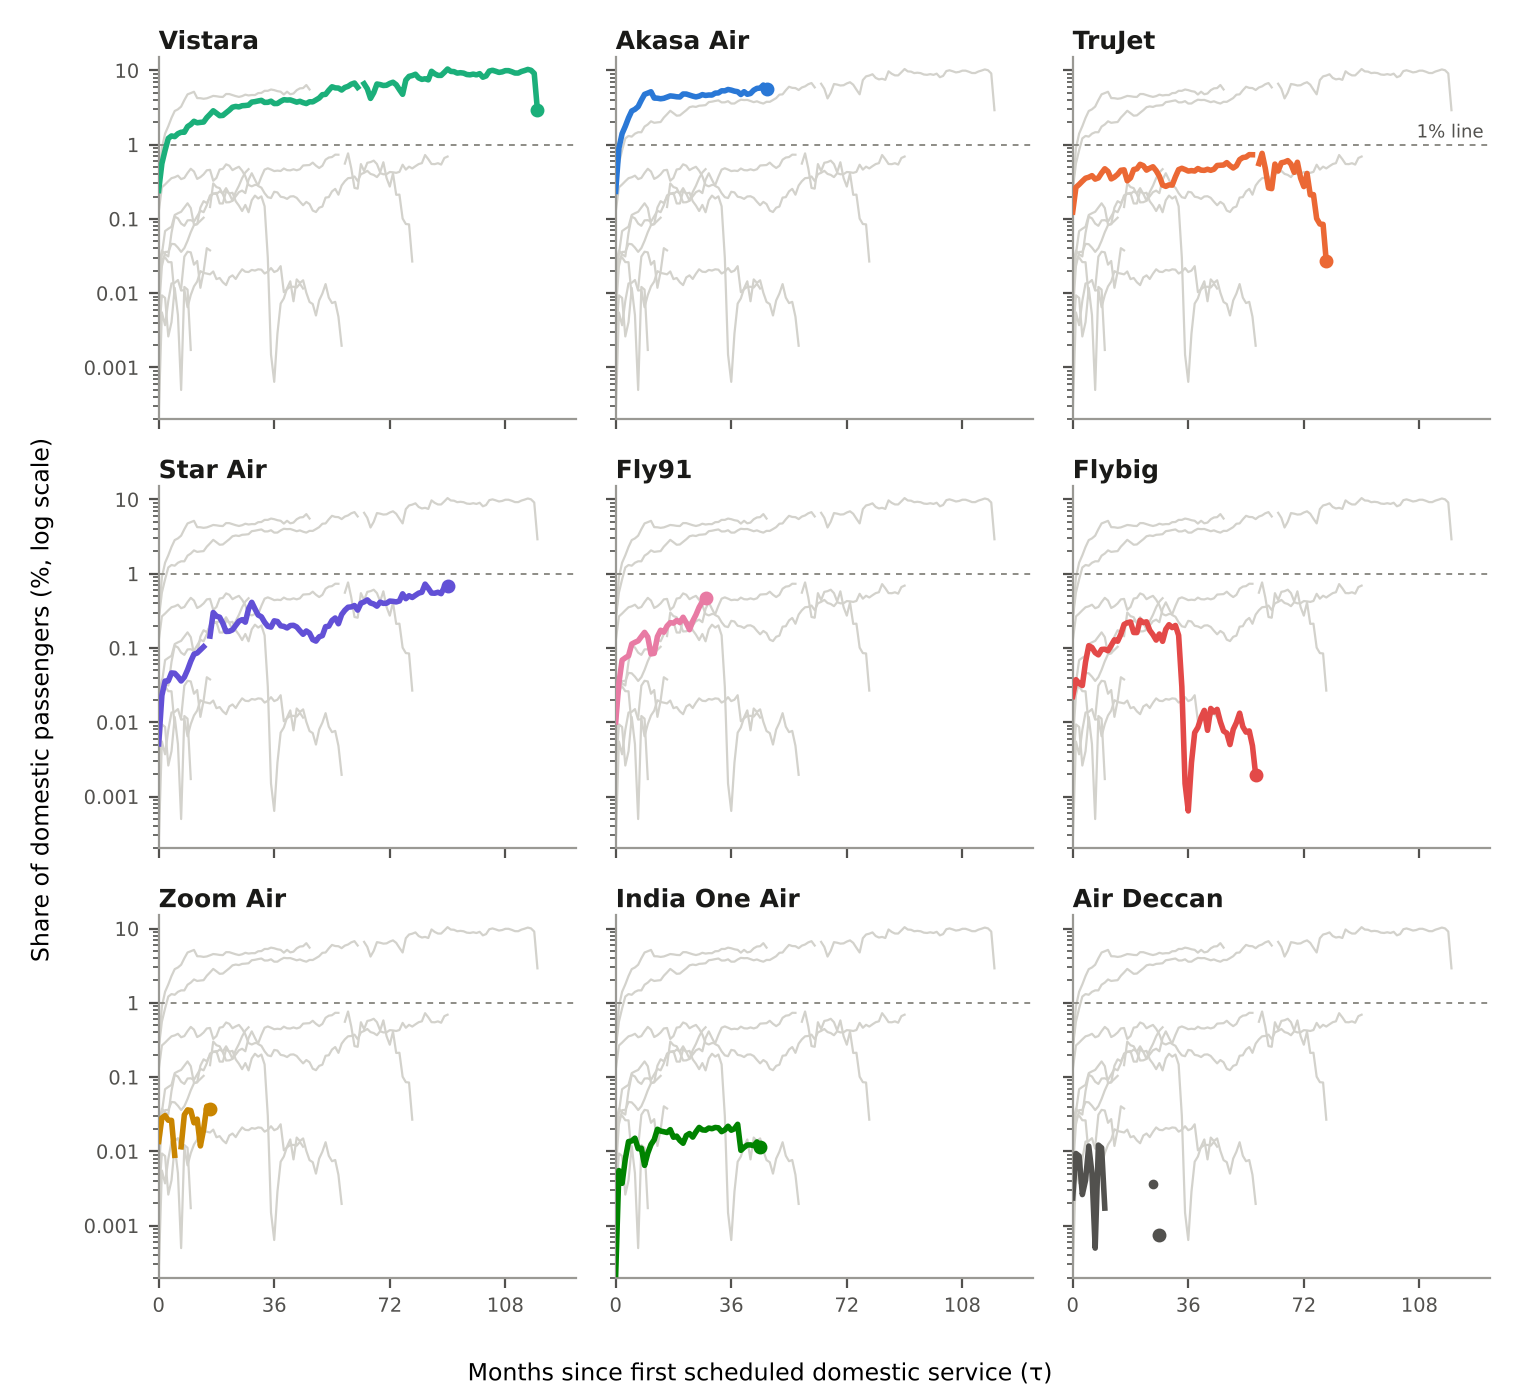
\includegraphics[width=0.82\textwidth]{figures/fig_o3_age.png}
\captionof{figure}{O3: Passenger share of the nine entrants by months since first service (log scale). One panel per entrant (coloured); the other eight are shown in grey for reference, and the dashed line marks 1\%. Each line ends at the airline's last observed month; gaps are months missing from the data (April 2020 for Vistara, TruJet and Star Air). Shares below 0.0002\% are drawn at the axis floor, and Vistara's last point (November 2024) is a partial month. Source: DGCA via Kubicek (2026); authors' calculations.}
\label{fig:o3-age}
\end{minipage}\par\medskip

\textbf{Result 1: only two entrants achieved meaningful and persistent national market shares.} The 1\% market-share and 24-month persistence thresholds are study-defined measures, not industry standards. Only Vistara and Akasa Air ever exceeded 1\% of domestic passenger traffic. Together, they accounted for 93\% of the passengers carried by the nine entrants, while the other seven collectively never exceeded 1.17\% of national passenger traffic in any month. Akasa Air crossed the 1\% threshold in its third month of operations and Vistara in its fourth. Both maintained a share of at least 1\% for almost their entire observed operating periods: 46 of 48 months for Akasa Air and 115 of 118 months for Vistara. Both therefore meet the study's persistence criterion (Figure~\ref{fig:o3-age}). Akasa Air also grew faster, reaching a 5.43\% share at $\tau=36$, compared with Vistara's 3.58\% (Table~\ref{tab:o3-summary}). By contrast, all four entrants that ceased flying: TruJet, Flybig, Zoom Air and Air Deccan, had peak national shares below 0.8\%.

\textbf{Result 2: regional entrants established local route positions without gaining national scale.} Table~\ref{tab:o3-routes} measures each entrant's share of recorded weekly scheduled departures on its airport pairs; these figures represent scheduled capacity presence, not passenger market share. Vistara was the only recorded operator on just 1 of its 62 pairs, while Akasa Air held this position on 2 of 57. In contrast, the seven regional entrants were the sole recorded operators on 74 of their 106 pairs (70\%) and accounted for at least half of scheduled departures on 81 pairs (76\%). TruJet's monthly filings provide a further indication of this local concentration: in November 2019, it accounted for at least half of recorded flights on 17 of the 22 pairs that could be screened. On Chennai--Salem, it operated all 60 recorded flights (route \HHI{} of 10,000), despite the route carrying only 3,281 passengers across all airlines and TruJet holding just 0.63\% of the national market.

The scale entrants, meanwhile, competed alongside other airlines on most of their routes. Monthly data show Vistara's share of Mumbai--Delhi scheduled flights increasing from 20.01\% in April 2019 to 31.27\% in February 2024, while Akasa Air's share rose from 2.65\% in December 2022 to 8.75\% in July 2026. Across the major routes examined, Vistara's share increased on 16 of 20 routes, compared with 10 of 18 for Akasa Air. Taken together, these findings distinguish two forms of competitive presence: the regional entrants often occupied dominant positions on a limited number of routes, whereas the two scale entrants built substantial shares of the national passenger market. These route comparisons are not matched by airline age and cover different observation periods. Route \HHI{} also treats Vistara and Air India as separate firms, although both were Tata-owned by 2023. Zoom Air's route evidence is particularly limited, covering only two airport pairs.
% >>> LARGE TABLE: candidate to move to Appendix B (keep the \label; the text refers to it by \ref).
\begin{minipage}{\textwidth}
\footnotesize
\captionof{table}{O3: Route presence of the nine entrants from schedule snapshots}
\label{tab:o3-routes}
\setlength{\tabcolsep}{3pt}\fontsize{10}{12}\selectfont\setstretch{1}\setlength{\tabcolsep}{3pt}
\renewcommand{\arraystretch}{1.15}
\begin{tabular}{|>{\raggedright\arraybackslash}p{\dimexpr0.18\linewidth-2\tabcolsep-1.125\arrayrulewidth\relax}|>{\raggedright\arraybackslash}p{\dimexpr0.18\linewidth-2\tabcolsep-1.125\arrayrulewidth\relax}|>{\raggedright\arraybackslash}p{\dimexpr0.08\linewidth-2\tabcolsep-1.125\arrayrulewidth\relax}|>{\raggedright\arraybackslash}p{\dimexpr0.12\linewidth-2\tabcolsep-1.125\arrayrulewidth\relax}|>{\raggedright\arraybackslash}p{\dimexpr0.11\linewidth-2\tabcolsep-1.125\arrayrulewidth\relax}|>{\raggedright\arraybackslash}p{\dimexpr0.08\linewidth-2\tabcolsep-1.125\arrayrulewidth\relax}|>{\raggedright\arraybackslash}p{\dimexpr0.13\linewidth-2\tabcolsep-1.125\arrayrulewidth\relax}|>{\raggedright\arraybackslash}p{\dimexpr0.12\linewidth-2\tabcolsep-1.125\arrayrulewidth\relax}|}
\hline
\textbf{Airline} & \textbf{Snapshot} & \textbf{Pairs} & \textbf{Weekly deps.} & \textbf{$\geq$50\%} & \textbf{Sole} & \textbf{Median (\%)} & \textbf{Airlines} \\
\hline
Vistara & Winter 2023 & 62 & 1999 & 3 & 1 & 20.4 & 9 \\
\hline
Akasa Air & Summer 2026 & 57 & 1076 & 7 & 2 & 23.1 & 9 \\
\hline
TruJet & Winter 2021 & 29 & 457 & 21 & 17 & 100.0 & 10 \\
\hline
Star Air & Summer 2026 & 37 & 387 & 30 & 28 & 100.0 & 9 \\
\hline
Fly91 & Summer 2026 & 14 & 249 & 9 & 8 & 100.0 & 9 \\
\hline
Flybig & Summer 2022 & 12 & 158 & 9 & 9 & 100.0 & 9 \\
\hline
Zoom Air & Winter 2017 & 2 & 28 & 1 & 1 & 66.7 & 11 \\
\hline
India One Air & Summer 2026 & 7 & 126 & 7 & 7 & 100.0 & 9 \\
\hline
Air Deccan & Winter 2019 & 5 & 54 & 4 & 4 & 100.0 & 11 \\
\hline
\end{tabular}
\par\raggedright\footnotesize
Notes: Pairs are airport pairs served. $\geq$50\% and Sole count pairs where the entrant accounted for at least half, or all, of recorded weekly scheduled departures, respectively. Median is the median entrant share across its pairs. Airlines is the number of airlines with recorded filings in that season. Snapshots use the mid-season date (15 January or 15 July) from the entrant's latest usable filing before closure or merger, or the latest available filing. Shares are based on recorded weekly departures, with both directions pooled. Source: DGCA-approved domestic schedules; authors' calculations.
\end{minipage}\par\medskip

\textbf{Result 3: Financial performance and funding of the two scale entrants.} Vistara and Akasa Air are examined here because they were the only two entrants to exceed 1\% of domestic passenger traffic, reaching peak shares of 10.44\% and 6.36\%, respectively. Their sustained market presence makes them the clearest cases for examining whether scale translated into financial viability. The seven regional entrants did not reach the 1\% threshold; their financial evidence is discussed in Results 4 and 5.

As shown in Table~\ref{tab:o3-fin}, both airlines recorded substantial revenue growth, but their margin trajectories differed. Vistara's revenue grew by 24.87\%, while its net margin improved from $-11.36\%$ to $-3.80\%$, a gain of 7.57 percentage points. Akasa Air's revenue grew faster, by 34.59\%, but its net margin deteriorated slightly from $-43.28\%$ to $-44.03\%$. Thus, revenue growth did not necessarily translate into improved profitability. Akasa Air's FY2026 loss of Rs~2,716 crore is equivalent to approximately Rs~3,150 per domestic passenger carried (8.6 million). This is only an indicative comparison, since the reported loss also includes its international operations.

To illustrate the scale of the losses, even under a hypothetical 100\% incremental contribution margin, additional revenue equal to the accounting loss would be required to offset it: Rs~2,716 crore for Akasa Air (approximately 44\% of its FY2026 revenue) and Rs~581 crore for Vistara (approximately 3.8\% of its FY2024 revenue). These are illustrative lower-bound estimates. At contribution margins below 100\%, the additional revenue required would be higher, assuming other costs remain unchanged.

Both airlines also incurred substantial losses in their early years. Vistara's DGCA-reported operating result was negative in each of FY2017--FY2019, with operating margins ranging from $-39.5\%$ to $-24.2\%$ (Rajya Sabha, 2019). Akasa Air reported a loss of Rs~1,669.59 crore in FY2024 in the Ministry's data. Their continued operations therefore depended on access to funding as well as revenue growth. ICRA notes that equity infusions and aircraft sale-and-leaseback proceeds supported Akasa Air's continuing losses (ICRA, 2026). In Vistara's case, its owners described the merger with Air India as a way to combine Air India's slots and traffic rights with Vistara's customer base and capabilities (Singapore Airlines, 2022).

\begin{minipage}{\textwidth}
\footnotesize
\captionof{table}{O3: Audited results and funding evidence for Vistara and Akasa Air, the two entrants above 1\% of passengers}
\label{tab:o3-fin}
\fontsize{10}{12}\selectfont\setstretch{1}\setlength{\tabcolsep}{3pt}
\renewcommand{\arraystretch}{1.15}
\begin{tabular}{|>{\raggedright\arraybackslash}p{\dimexpr0.3\linewidth-2\tabcolsep-1.3333333333333333\arrayrulewidth\relax}|>{\raggedright\arraybackslash}p{\dimexpr0.35\linewidth-2\tabcolsep-1.3333333333333333\arrayrulewidth\relax}|>{\raggedright\arraybackslash}p{\dimexpr0.35\linewidth-2\tabcolsep-1.3333333333333333\arrayrulewidth\relax}|}
\hline
 & \textbf{Vistara (FY2023$\to$FY2024)} & \textbf{Akasa Air (FY2025$\to$FY2026)} \\
\hline
Operating income (Rs crore) & 12,261.4 $\to$ 15,310.3 & 4,582.7 $\to$ 6,167.9 \\
\hline
Profit after tax (Rs crore) & $-1{,}393.3\to-581.1$ & $-1{,}983.5\to-2{,}716.0$ \\
\hline
Net margin & $-11.36\%\to-3.80\%$ & $-43.28\%\to-44.03\%$ \\
\hline
Year-3 load factor & 84.67\% & 91.01\% \\
\hline
Funding & Rs~10,020 crore from Tata and Singapore Airlines by Aug 2024 & Equity round completed 19 Aug 2025; about US\$125 million is a press estimate \\
\hline
\end{tabular}
\end{minipage}\par\medskip

\textbf{Result 4: the regional entrants' financial records show a mix of losses, small profits and funding support, with no clear relationship to market share.} Table~\ref{tab:o3-fy25} compiles the available public financial figures for the seven regional entrants. Although each has at least one reported figure, the data are not available on a consistent basis: they include Ministry of Civil Aviation net profits after tax for FY2023--FY2025 (with FY2025 figures provisional) and DGCA operating results for FY2017--FY2021 (Ministry of Civil Aviation, 2025; Rajya Sabha, 2019, 2021). Comparisons are therefore restricted to figures reported on the same basis.

FY2024--25 provides a useful, though limited, comparison among operating entrants. Fly91 reported a loss of Rs~67.65 crore, while Star Air and India One Air reported profits of Rs~68.75 crore and Rs~3.34 crore, respectively. Akasa Air, the larger scale entrant, reported a loss of Rs~1,986.25 crore in the same Ministry dataset. These figures illustrate the variation in reported financial outcomes but are insufficient to establish a relationship between profitability and market share. Both profitable regional carriers had reported losses in the preceding two years. Moreover, Star Air's FY2025 profit was smaller than the approximately Rs~200 crore in UDAN viability gap funding it reportedly received that year (Aviation A2Z, 2026). This is a descriptive comparison only: the available evidence does not establish how the funding was accounted for or what the airline's result would have been without it.

Financial evidence for the entrants that ceased operations covers only parts of their operating histories. TruJet's reported operating margin improved from $-64.0\%$ in FY2017 to $-15.5\%$ in FY2019 (provisional), but a later parliamentary reply records an operating loss of Rs~143.16 crore in FY2021, a year before it ceased flying (Rajya Sabha, 2021). Zoom Air's operating margin moved from $+4.7\%$ to $-13.5\%$ in its final reported year. Air Deccan reported negative operating results in both available years, although these figures may include non-scheduled operations. Flybig, by contrast, reported net profits in FY2023 and FY2024, but no FY2025 figure is available. TruJet's funding difficulties provide further context: a 2021 report stated that an agreed investment had not materialised and that its main investor had returned ownership to the founder. By February 2022, reports described widespread groundings, with only one aircraft still flying (Hindu BusinessLine, 2021; ch-aviation, 2022). The Comptroller and Auditor General of India's UDAN audit records 52 route awards and 42 commencements for TruJet, but no routes operational as of March 2023 (CAG, 2023).

\textbf{Result 5: local dominance and reported profits did not guarantee regional entrants' survival.} Table~\ref{tab:o3-seven} compares the seven regional entrants across traffic history, peak national share, route presence and reported financial outcomes. The four entrants that ceased flying: TruJet, Flybig, Zoom Air and Air Deccan, were the sole recorded operators on 31 of their 48 route-snapshot pairs (65\%). Thus, even substantial local presence did not ensure continued operations. Reported profits were not a guarantee of survival either: Flybig recorded net profits in FY2023 and FY2024, while Zoom Air reported positive operating results in FY2017 and FY2018, yet both subsequently ceased flying. TruJet, in contrast, reported operating losses in all the years for which figures are available.

The three regional entrants still operating at the July 2026 study cutoff also differed considerably in their observed scale. Star Air had recorded passenger traffic for 90 months and reached a peak national share of 0.73\%; Fly91 had operated for 29 traffic months and reached 0.47\%; and India One Air had recorded traffic for 46 months but remained near 0.02\%. These seven cases suggest that neither local route dominance nor isolated years of reported profit were sufficient to ensure survival. However, the small sample, incomplete financial records and differences in operating age do not allow the analysis to identify why some entrants survived while others exited.

\begin{minipage}{\textwidth}
\footnotesize
\setlength{\tabcolsep}{3pt}
\captionof{table}{O3: The seven regional entrants compared}
\label{tab:o3-seven}
\fontsize{10}{12}\selectfont\setstretch{1}\setlength{\tabcolsep}{3pt}
\renewcommand{\arraystretch}{1.15}
\begin{tabular}{|>{\raggedright\arraybackslash}p{\dimexpr0.13\linewidth-2\tabcolsep-1.2\arrayrulewidth\relax}|>{\raggedright\arraybackslash}p{\dimexpr0.18\linewidth-2\tabcolsep-1.2\arrayrulewidth\relax}|>{\raggedright\arraybackslash}p{\dimexpr0.11\linewidth-2\tabcolsep-1.2\arrayrulewidth\relax}|>{\raggedright\arraybackslash}p{\dimexpr0.23\linewidth-2\tabcolsep-1.2\arrayrulewidth\relax}|>{\raggedright\arraybackslash}p{\dimexpr0.35\linewidth-2\tabcolsep-1.2\arrayrulewidth\relax}|}
\hline
\textbf{Airline} & \textbf{Traffic months (outcome)} & \textbf{Peak share (\%)} & \textbf{Route snapshot: pairs; $\geq$50\%; sole} & \textbf{Reported financial results (Rs crore)} \\
\hline
TruJet & 79, Jul 2015--Feb 2022 (ceased) & 0.76 & 29; 21; 17 (winter 2021) & $-80.77$, $-85.15$, $-41.00$ (FY2017--19, operating); later years in Table~\ref{tab:o3-fy25} \\
\hline
Star Air & 90, from Jan 2019 (operating) & 0.73 & 37; 30; 28 (summer 2026) & $-20.84$, $-33.31$, $+68.75$ (FY2023--25, net) \\
\hline
Fly91 & 29, from Mar 2024 (operating) & 0.47 & 14; 9; 8 (summer 2026) & $-31.42$, $-67.65$ (FY2024--25, net) \\
\hline
Flybig & 58, Jan 2021--Oct 2025 (ceased) & 0.24 & 12; 9; 9 (summer 2022) & $+5.59$, $+4.83$ (FY2023--24, net); none for FY2025 \\
\hline
Zoom Air & 16, Feb 2017--Jun 2018 (ceased) & 0.04 & 2; 1; 1 (winter 2017) & $+0.14$, $+0.81$, $-1.40$ (FY2017--19, operating) \\
\hline
India One Air & 46, from Oct 2022 (operating) & 0.02 & 7; 7; 7 (summer 2026) & $-8.73$, $-3.23$, $+3.34$ (FY2023--25, net) \\
\hline
Air Deccan & 13, Dec 2017--Mar 2020 (ceased) & 0.01 & 5; 4; 4 (winter 2019) & $-13.55$, $-28.90$ (FY2018--19, operating) \\
\hline
\end{tabular}
\par\raggedright\footnotesize Sources: DGCA via Kubicek (2026); DGCA-approved domestic schedules; Ministry of Civil Aviation (2025); Rajya Sabha (2019); authors' calculations. Route snapshot columns are defined under Table~\ref{tab:o3-routes}. Financial figures are reported on different bases; see Table~\ref{tab:o3-fy25}.
\end{minipage}\par\medskip
\end{mergedcontribution}

\FloatBarrier
\clearpage
\begin{mergedcontribution}{authorGoutham}
\subsection{O4: Concentration and resilience}
\label{sec:o4-results}
\subsubsection{National concentration}
Table~\ref{tab:o4-national-results} compares the full national series with the focus period. The joint condition requires IndiGo and Air India Group to be the two largest groups, with CR2 of at least 80\% and a share gap above 20 percentage points in the same month. Appendix~\ref{app:o4-national-calculations} provides the formulas and a worked example for the measures in Table~\ref{tab:o4-national-results}.

\begin{resultstable}{National concentration conditions: January 2015--July 2026 and the December 2024--July 2026 focus period.}{tab:o4-national-results}
\centering
\begin{tabularx}{\linewidth}{|>{\raggedright\arraybackslash}X|r|r|r|}
\hline
\textbf{Condition} & \textbf{\shortstack{\strut Full series\\\strut Months / 138}} & \textbf{\shortstack{\strut Focus period\\\strut Months / 20}} & \textbf{\shortstack{\strut Focus period\\\strut Range}} \\
\hline
IndiGo and AI Group are the two largest groups & 59/138 & 20/20 & -- \\
\hline
CR2 $\geq 80\%$ & 48/138 & 20/20 & 89.13--91.70\% \\
\hline
Share gap $>20$ pp & 120/138 & 20/20 & 30.01--43.39 pp \\
\hline
All three conditions together & 48/138 & 20/20 & -- \\
\hline
\end{tabularx}
\par
\resultstablenotes{Counts show qualifying months divided by observed months. April 2020 is unavailable. AI Group means Air India Group; pp means percentage points.}{DGCA monthly airline data via Kubicek (2026); authors' calculations.}
\end{resultstable}

\subsubsection{Route concentration and national comparison}
Table~\ref{tab:o4-route-results} reports the full-period results for the selected 20 airport pairs. Each observation represents one airport pair in one month. Shares are calculated from approved scheduled flights in both directions.

\begin{resultstable}{Route concentration and IndiGo dependence, April 2019--September 2026.}{tab:o4-route-results}
\centering
\begin{tabularx}{\linewidth}{|>{\raggedright\arraybackslash}X|r|r|}
\hline
\textbf{Measure} & \textbf{Observations} & \textbf{Percentage (\%)} \\
\hline
Ownership HHI $>1{,}800$ & 1,143/1,150 & 99.39 \\
\hline
IndiGo and AI Group are the unique top two & 730/1,150 & 63.48 \\
\hline
IndiGo--AI Group leading pair, CR2 $\geq80\%$ and gap $>20$ pp & 95/1,150 & 8.26 \\
\hline
IndiGo supplies $\geq60\%$ of scheduled flights & 79/1,150 & 6.87 \\
\hline
IndiGo is the sole scheduled operator & 0/1,150 & 0.00 \\
\hline
\end{tabularx}
\par
\resultstablenotes{The joint condition allows either group to lead. A tie for second place prevents a unique leading pair. AI Group means Air India Group; pp means percentage points.}{DGCA approved domestic schedules; authors' calculations.}
\end{resultstable}

\medskip
\begin{minipage}{\linewidth}
\setlength{\parskip}{6pt}
For the focus period, Table~\ref{tab:o4-route-focus} compares national results with the top 20 and top 10 busiest airport pairs. National shares measure passengers, while airport-pair shares measure scheduled flights.

\begin{resultstable}{National and airport-pair concentration during December 2024--July 2026.}{tab:o4-route-focus}
\centering
\begin{tabularx}{\linewidth}{|>{\raggedright\arraybackslash}X|r|r|r|}
\hline
\textbf{Measure} & \textbf{\shortstack{\strut National\\\strut Passenger data}} & \textbf{\shortstack{\strut Top 20\\\strut airport pairs\\\strut Scheduled flights}} & \textbf{\shortstack{\strut Top 10\\\strut airport pairs\\\strut Scheduled flights}} \\
\hline
IndiGo and AI Group are the unique top two & 20/20 & 328/350 & 184/184 \\
\hline
Median CR2 (\%) & 90.91 & 89.55 & 89.37 \\
\hline
Median share gap (pp) & 37.35 & 11.92 & 7.69 \\
\hline
Median fringe share (\%) & 9.09 & 10.45 & 10.63 \\
\hline
Leading pair, CR2 $\geq80\%$ and gap $>20$ pp, with IndiGo first & 20/20 & 50/350 & 9/184 \\
\hline
\end{tabularx}
\par
\resultstablenotes{National results use 20 monthly observations. Each route-level observation represents one airport pair in one month. Over these 20 months, the top-20 sample has usable data for 350 of 400 possible observations ($20\times20$), and the top-ten sample has 184 of 200 ($10\times20$). Missing observations are excluded. AI Group means Air India Group; pp means percentage points.}{DGCA monthly airline data via Kubicek (2026) and approved domestic schedules; authors' calculations.}
\end{resultstable}
\end{minipage}
\par\addvspace{6pt}

During the focus period, median CR2 is similar nationally and on the top 20 and top 10 busiest airport pairs, at around 89--91\%. However, the median gap between the two largest groups is 37.35 percentage points nationally, compared with 11.92 on the top 20 airport pairs and 7.69 on the top 10. Appendix~\ref{app:o4-route-preparation} provides the detailed results, coverage checks, leadership counts and worked calculations.

\subsubsection{Rivals' capacity buffer}
Table~\ref{tab:o4-capacity-buffer} compares the two Decembers. Rivals include all retained airlines other than IndiGo. Their combined ASK minus RPK gives unused capacity, which is expressed as a percentage of IndiGo's RPK.

\begin{resultstable}{Rivals' capacity buffer, December 2024 and December 2025.}{tab:o4-capacity-buffer}
\centering
\begin{tabularx}{\linewidth}{|>{\raggedright\arraybackslash}X|r|r|r|}
\hline
\textbf{Measure} & \textbf{Dec 2024} & \textbf{Dec 2025} & \textbf{Change} \\
\hline
Rivals' ASK (billion seat-km) & 6.385 & 6.619 & +0.234 \\
\hline
Rivals' RPK (billion passenger-km) & 5.493 & 5.947 & +0.454 \\
\hline
Rivals' unused capacity (billion seat-km) & 0.892 & 0.672 & -0.220 \\
\hline
IndiGo RPK (billion passenger-km) & 9.113 & 8.208 & -0.905 \\
\hline
Buffer relative to IndiGo (\%) & 9.79 & 8.19 & -1.60 pp \\
\hline
\end{tabularx}
\par
\resultstablenotes{Changes are December 2025 minus December 2024, calculated before rounding. ASK measures available seat-kilometres and RPK measures revenue passenger-kilometres. The buffer change is in percentage points (pp).}{DGCA monthly airline data via Kubicek (2026); authors' calculations.}
\end{resultstable}

Rivals' passenger traffic rises by more than their offered capacity, reducing unused capacity. These monthly totals do not establish whether seats were available on the routes and dates affected by cancellations. Appendix~\ref{app:o4-capacity-buffer} provides the airline-level inputs and worked calculation.
\end{mergedcontribution}

\clearpage
\section{Discussion}
\label{sec:review-discussion}
\subsection{Economic interpretation}
\begin{mergedcontribution}{authorSowmya}
\subsubsection{O1: Concentration and ownership effects}
\textbf{From oligopoly towards asymmetric duopoly.} Ownership-HHI rose from a mean of 2,408 before the Jet Airways exit to 4,877 after the mergers, equivalent to falling from 4.2 to 2.1 equal-sized airlines; nine in ten passengers now fly IndiGo or the Air India Group. Concentration never left the highly concentrated band, so what changed is the distance above it, and it changed in steps tied to exits and changes of control rather than through gradual drift (Tables~\ref{tab:o1-periods}, \ref{tab:o1-drift} and~\ref{tab:o1-regression}).

\textbf{Ownership matters more than brands.} The Tata acquisition is the largest step (about 900 points), and half of it is the Grouping Effect: brands that remained separate in DGCA reports came under one owner. Brand shares alone would understate that step by half. Partial ownership is small: the wedge averages 23 points before 2022 and never exceeds 77 (Tables~\ref{tab:o1-gap} and~\ref{tab:review-o1-wedge}).

\textbf{Course lenses.} Read through structure--conduct--performance \parencite{gandhi2026marketstructure}, the rise signals greater potential market power. Under Cournot competition the industry Lerner index is $(\mathrm{HHI}/10{,}000)/|\varepsilon|$; with $|\varepsilon|=1.5$ the permanent drifts D1 and D5 imply margins 3.5 and 4.6 points higher (using the drift-point HHI changes in Table~\ref{tab:o1-drift}). This is an implication of structure, not a measured markup. IndiGo's large aircraft orders act as Stackelberg-style capacity commitments, and its share rose from 57.5\% to 63.2\% across D5 and was held. Both exits occurred with HHI already above 1,800, and Akasa Air's entry in August 2022 was followed only by a slow fall of about 390 points over six months, so entry has not offset consolidation.

\textbf{Supplementary grouping-gap comparison.} The gap is always $\geq0$. Its changes are $+316$ at D4 and $-100$ at D6, compared with $-27$ and $+29$ at the exits (Table~\ref{tab:o1-drift}). The wedge changes no month's concentration classification. The event steps remain significant with 6 or 18 lags and with COVID months dropped ($t\geq2.2$), and CR2 agrees (Tables~\ref{tab:o1-robust} and~\ref{tab:o1-cr2reg}). These are dated level shifts in national structure, not causal estimates of effects on fares, profits or passengers.
\end{mergedcontribution}

\begin{mergedcontribution}{authorMeena}
\subsubsection{O2: Exits and Tata consolidation}
\textbf{Exits.} Jet Airways' and Go First's exits reduced the effective number of equal-sized firms from 4.1 to 3.5 and 2.5 to 2.2, respectively. In the Cournot model, firms choose quantities simultaneously, taking rivals' output as given. Applied to our study, this would mean each airline decides how many seats to offer, assuming its competitors keep their seat numbers unchanged. Holding demand elasticity fixed, higher concentration implies a higher share-weighted markup:
\[
\overline{L} = \frac{\HHI/10{,}000}{|\varepsilon|},
\]
where $\overline{L}$ is the share-weighted price--cost markup as a fraction of price, and $|\varepsilon|$ is absolute market demand elasticity. An illustrative elasticity of 1.5 implies markup increases of about 3.0 and 4.6 percentage points of price, not observed fare increases: we have no fare data. The exit-window results are in Tables~\ref{tab:o2-absorption} and~\ref{tab:review-o2-capacity-contribution}. Worked calculations are in Appendix~\ref{app:workings}, part~C.

\textbf{Why IndiGo absorbed most.} In the Stackelberg model, a leader commits to its output first, anticipating how rivals will respond; followers then choose their output after observing that commitment. Applied to our study, this would mean IndiGo commits to future capacity first, and rivals plan their own expansion around that commitment. Its June 2023 order for 500 aircraft fits this interpretation, rather than proving the model describes actual behaviour. Slot access also constrains rivals' expansion: SpiceJet received vacated Jet Airways slots and expanded capacity, illustrating an entry barrier. IndiGo's dominance may reflect cost leadership as well as weaker competition; without fare and cost data, we cannot distinguish them.

\textbf{Tata consolidation and merger review.} For each set of entities combined, the fixed-share concentration effect is
\[
\Delta\HHI_{\text{mechanical}} = \left(\sum_i s_i\right)^2 - \sum_i s_i^2,
\]
where $s_i$ are pre-consolidation percentage shares, held fixed; effects are summed across separate mergers. Applied to our study, this means concentration can rise simply because airlines are counted as one entity rather than separate competitors, even if none gains any passengers. Common ownership accounts for most of the January 2022 rise; the late-2024 mergers mechanically added 256 brand \HHI{} points (worked calculations in Appendix~\ref{app:workings}, part~B). CCI's capacity commitments protected seven routes but did not address national concentration. Both perspectives matter: with two groups carrying about 90\% of passengers, national structure also affects slot access and exposure to single-airline disruption.
\end{mergedcontribution}

\begin{mergedcontribution}{authorSweta}
\subsubsection{O3: Entrant scale and financial viability}
\label{sec:review-o3-interpretation}
Nine entrants entered India's domestic aviation market over the eleven-and-a-half-year study period, but only two achieved meaningful and persistent national market shares. Vistara subsequently merged with Air India in November 2024, leaving Akasa Air as the only scale entrant continuing to expand as an independent competitor at the July 2026 cutoff. This suggests that entry alone did not ensure effective competition; entrants needed to build sufficient traffic and sustain operations over time (Tables~\ref{tab:o3-summary} and~\ref{tab:o3-routes}).

The findings are broadly consistent with the cost structure described by $AC=F/Q+v$. Higher passenger volumes can spread fixed costs over a larger output base, while better aircraft utilisation can improve the economics of operations. The load-factor evidence illustrates this difference: Vistara's load factor increased from 65.6\% in its first year to 84.7\% in its third, while Akasa Air recorded 84.7\% and 91.0\%, respectively. TruJet, by comparison, recorded 80.1\% in its first year and 76.6\% in its third. Although these figures are consistent with the potential benefits of higher utilisation, they do not establish that load factor or scale caused the different outcomes. TruJet's experience also shows why local route dominance is not equivalent to national scale: it held a dominant position on several routes, but the routes themselves carried relatively few passengers. A high share of a small market may therefore provide insufficient traffic to support the broader cost structure of an airline.

The financial results further qualify the relationship between growth and viability. Vistara's margins improved as revenue expanded, whereas Akasa Air's faster revenue growth was accompanied by continued substantial losses. Its continued expansion alongside these losses indicates the importance of access to external capital, but funding availability should not be interpreted as evidence of financial self-sufficiency. More generally, accounting results do not capture the full economic cost of capital; economic profitability would also require a return sufficient to compensate investors for the opportunity cost of their funds (Tables~\ref{tab:o3-fin} and~\ref{tab:o3-seven}).

Overall, the evidence supports the expectation that only entrants achieving sufficient scale and sustained passenger volumes became meaningful national competitors. It also shows that local route dominance and revenue growth alone were insufficient indicators of financial viability or survival. However, the analysis is descriptive: it identifies patterns consistent with the economic framework and existing literature, rather than testing whether economies of scale, funding or route concentration caused individual entrant outcomes.
\end{mergedcontribution}

\begin{mergedcontribution}{authorGoutham}
\subsubsection{O4: Concentration and resilience}
\textbf{National market structure.} During the focus period (December 2024 to July 2026), the national results are consistent with an asymmetric duopoly. IndiGo and Air India Group dominate the market, but IndiGo has a much larger passenger share (Tables~\ref{tab:o4-national-results} and~\ref{tab:o4-route-focus}). Other airlines form a small competitive fringe. This indicates that domestic passenger traffic depends heavily on two ownership groups, particularly IndiGo, despite the presence of several smaller airlines.

\textbf{Competition on individual airport pairs.} Table~\ref{tab:o4-route-focus} shows that IndiGo and Air India Group, the two national leaders, also dominate scheduled flights on the top 20 and top 10 busiest airport pairs. However, the median gap between the two largest groups is smaller than nationally. This highlights the importance of market definition: IndiGo's large national lead does not imply an equally large lead on individual airport pairs. Note that national shares use passenger counts, while airport-pair shares use scheduled-flight frequencies, reflecting the data available for each.

\textbf{Rivals' capacity buffer.} Table~\ref{tab:o4-capacity-buffer} shows that rivals' unused capacity relative to IndiGo's traffic fell from 9.79\% in December 2024 to 8.19\% in December 2025. This provides a rough aggregate measure of the spare capacity elsewhere in the market relative to IndiGo's traffic, indicating a smaller buffer in December 2025. However, unused seats would also need to match affected passengers' routes and travel dates, so the ratio cannot directly estimate how many passengers could have been accommodated.
\end{mergedcontribution}

\FloatBarrier
\clearpage
\subsection{Hypotheses revisited}
\label{sec:review-hypothesis-outcomes}
Table~\ref{tab:hypotheses} links the hypothesis outcomes to the results in Section~5. Full hypothesis statements are given in Section~\ref{sec:hypotheses}. H1--H2 concern ownership effects, H3--H4 concern exits, and H5--H7 concern concentration and capacity. O3's entrant-scale expectation is discussed in Section~\ref{sec:review-o3-interpretation}.
\begin{resultstable}{Hypothesis outcomes and supporting evidence.}{tab:hypotheses}
\centering
\fontsize{10}{12}\selectfont\setstretch{1}\setlength{\tabcolsep}{4pt}\renewcommand{\arraystretch}{1.15}
\begin{tabular}{|>{\raggedright\arraybackslash}p{\dimexpr0.23\linewidth-2\tabcolsep-1.3333333333333333\arrayrulewidth\relax}|>{\raggedright\arraybackslash}p{\dimexpr0.23\linewidth-2\tabcolsep-1.3333333333333333\arrayrulewidth\relax}|>{\raggedright\arraybackslash}p{\dimexpr0.54\linewidth-2\tabcolsep-1.3333333333333333\arrayrulewidth\relax}|}
\hline
\textbf{Hypothesis (objective)} & \textbf{Outcome} & \textbf{Supporting evidence from Section 5}\\
\hline
\textcolor{authorSowmya}{\textbf{H1 (O1)}\newline Lasting event steps} & \textcolor{authorSowmya}{Supported for exits and acquisition, weaker for legal mergers} & \textcolor{authorSowmya}{Drift changes are $+531$, $+367$ and $+693$ points for Jet, Tata and Go First. The fitted legal-merger step is smaller, at 137 points ($t=2.5$). Tables~\ref{tab:o1-drift} and~\ref{tab:o1-regression}.}\\
\hline
\textcolor{authorSowmya}{\textbf{H2 (O1)}\newline Partial-ownership wedge} & \textcolor{authorSowmya}{Partially supported, small magnitude} & \textcolor{authorSowmya}{The pre-2022 mean wedge is 22.9 points (0.8\% of Ownership-HHI), with a maximum of 76.6 (2.2\%); it vanishes from January 2022. Table~\ref{tab:review-o1-wedge}.}\\
\hline
\textcolor{authorMeena}{\textbf{H3 (O2)}\newline Exit absorption} & \textcolor{authorMeena}{Partially supported} & \textcolor{authorMeena}{IndiGo leads passenger absorption after both exits (37.7\% and 66.0\%). SpiceJet leads capacity absorption after Jet (30.4\%, versus IndiGo\textquotesingle s 28.5\%). Table~\ref{tab:o2-absorption}.}\\
\hline
\textcolor{authorMeena}{\textbf{H4 (O2)}\newline Contribution to the HHI rise} & \textcolor{authorMeena}{Supported} & \textcolor{authorMeena}{IndiGo adds 473 of 444 passenger-based HHI points after Jet and 632 of 690 after Go First. Capacity-based results are 352 of 354 and 599 of 653 points. Tables~\ref{tab:o2-absorption} and~\ref{tab:review-o2-capacity-contribution}.}\\
\hline
\textcolor{authorGoutham}{\textbf{H5 (O4)}\newline National concentration} & \textcolor{authorGoutham}{Supported} & \textcolor{authorGoutham}{All conditions hold in 20/20 focus-period months. Minimum CR2 is 89.13\% and the minimum share gap is 30.01 pp. Table~\ref{tab:o4-national-results}.}\\
\hline
\textcolor{authorGoutham}{\textbf{H6 (O4)}\newline Route concentration} & \textcolor{authorGoutham}{Supported} & \textcolor{authorGoutham}{HHI exceeds 1,800 in 1,143/1,150 airport-pair/month observations (99.39\%), more than half of the available sample. Table~\ref{tab:o4-route-results}.}\\
\hline
\textcolor{authorGoutham}{\textbf{H7 (O4)}\newline Rivals\textquotesingle\ capacity buffer} & \textcolor{authorGoutham}{Supported} & \textcolor{authorGoutham}{The ratio falls from 9.79\% in December 2024 to 8.19\% in December 2025, a decline of 1.60 pp. Table~\ref{tab:o4-capacity-buffer}.}\\
\hline
\end{tabular}
\resultstablenotes{O denotes the research objective; pp means percentage points. H1 uses the segmented-regression evidence and includes a weaker legal-merger result. H2's assessment reflects the small size of the partial-ownership effect. H5--H7 are descriptive checks, not significance tests or causal estimates. H5 uses December 2024--July 2026; H6 uses April 2019--September 2026. The H7 denominator is all IndiGo monthly RPK.}{Authors' results reported in Section~5.}
\end{resultstable}
\clearpage
\subsection{Connection to the literature review}
\begin{mergedcontribution}{authorSowmya}
\subsubsection{O1: Ownership structure and partial stakes}
Measuring concentration by owner requires knowing who controls each airline and who holds minority stakes in rivals \parencite{obriensalop2000}. Only two airlines had such cross-holdings before the Tata Group placed them in the Air India Group in January 2022 (schedule: Table~\ref{tab:o1-stakes}, Appendix~\ref{app:o1-stakes}).

\textbf{Vistara.} Tata Sons held 51\% from the start of the sample \parencite{sia2015annual,sia2022merger}. The other 49\% belonged to a foreign partner with no stake in any other Indian airline, so it adds no cross-holding term; it enters Equation~O1.1b only through the denominator of $\lambda$, diluting Tata's weight in Vistara's decisions.

\textbf{AirAsia India.} Tata Sons started at 30\% beside AirAsia Investment (49\%) and Telestra (21\%) \parencite{airasia2013jv}, rose to 41.06\% in 2015 and 49\% in March 2016 \parencite{tata2016airasia,airasia2018q4}, held 51\% by 2020, and reached 83.67\% after the December 2020 sale \parencite{airasia2021disposal,airasia2021results}.

\textbf{Inference.} Tata is the only owner with stakes in two rivals, so it alone creates the MHHI wedge: the more of AirAsia India it owns, the more Vistara internalises that rival's profit. The wedge therefore grows with Tata's stake, from about 1 point in 2015 (30\%) to 58 in 2021 (83.67\%), peaks at 76.6 points, and is zero from January 2022 when Tata controls both. At 0.8\% of Ownership-HHI on average, partial ownership matters far less than the full-control grouping of brands. Because stakes are company-reported rather than observed in operating decisions, MHHI measures structure, not conduct.
\end{mergedcontribution}

\begin{mergedcontribution}{authorMeena}
\subsubsection{O2: Concentration after airline exits}
The exit results match \textcite{grosche2020concentration}, who find that concentration in German air transport rose after Air Berlin's bankruptcy and that the largest group, Lufthansa, became more dominant, as IndiGo did here.
\end{mergedcontribution}

\begin{mergedcontribution}{authorSweta}
\subsubsection{O3: Entry, scale and viability}
These findings echo Oliveira and Oliveira (2018), who argue that market growth can attract new entrants but does not, by itself, ensure effective competition. Wang et al. (2018) associate low-cost competition in India with lower fares and higher demand, which is consistent with Akasa Air's rapid growth as a low-cost carrier. However, the present analysis focuses on entrant outcomes rather than estimating the causal effect of entry on fares or demand. Jayathilakan et al. (2024) find a positive association between revenue and passenger volume, but the cases examined here show that revenue growth does not necessarily translate into improved margins or long-term survival.

The findings also highlight the importance of how competition is measured. Brand-level measures, such as those discussed by Kumari et al. (2026), may count each entrant as a separate firm without reflecting substantial differences in their actual market presence. In this study, seven of the nine entrants never exceeded 1\% of national passenger traffic. Ownership and group affiliation also matter when interpreting concentration: Vistara was a Tata-linked joint venture in which Singapore Airlines held a 49\% stake (Tata Sons, 2024), and O1 groups it with the Air India Group from January 2022. Treating brands as independent competitors may therefore produce a different picture from one based on ownership groups. This distinction matters because brand-level market shares do not necessarily represent independent ownership-level competition, particularly after consolidation.
\end{mergedcontribution}

\begin{mergedcontribution}{authorGoutham}
\subsubsection{O4: Concentration and resilience}
\textcite{kumari2026soaring} examine how market concentration and operating efficiency relate to airline performance. Our study complements this work by comparing concentration nationally and on the busiest airport pairs. \textcite{gupta2025antitrust} discuss the risks of dependence on a dominant airline. The capacity-buffer comparison in Table~\ref{tab:o4-capacity-buffer} adds a quantitative measure of rivals' aggregate spare capacity relevant to that concern.
\end{mergedcontribution}


\clearpage
\section{Implications and Recommendations}
Discuss the implications of the findings for the relevant stakeholders.

Depending on the topic, these may include:
\templatebullet{Firms and managers}
\templatebullet{Consumers}
\templatebullet{Regulators}
\templatebullet{Policymakers}
\templatebullet{Industry participants}
Provide 2--3 specific recommendations where appropriate. Recommendations should follow from the findings of the study.

\clearpage
\section{Limitations}
\subsection{O4: Measurement and data availability}
Route concentration uses scheduled flights, which may differ from actual operations and do not account for aircraft size or occupancy. It therefore cannot establish how passengers are divided between airlines on each airport pair.

Rivals' unused capacity gives an overall indication of spare capacity elsewhere in the market relative to IndiGo's total monthly traffic. It cannot tell us how many passengers affected by cancellations could have been accommodated, because we do not know whether spare seats were available on the routes and dates they needed.

We could not obtain a consistent fare dataset for the study period. Our analysis therefore examines market structure through concentration and market shares, but cannot directly assess airlines' pricing power or whether greater concentration is associated with higher fares.

\section{Conclusion}
Summarise the research question, main findings, key economic interpretation, and main implications.

\newpage
\nocite{kubicek2026aviationstats,dgcaDomesticSchedules}
\printbibliography[title={References}]
\clearpage
\section*{O3 source references}
\begin{mergedcontribution}{authorSweta}
\begingroup\small\setstretch{1.0}\sloppy\emergencystretch=3em\def\UrlBreaks{\do\/\do\-\do\_\do\?\do\=\do\&\do\.\do\%}
\setlength{\parindent}{-0.5in}\setlength{\leftskip}{0.5in}\setlength{\parskip}{4pt}

Akasa Air. (2025a, August 19). \textit{Akasa Air announces completion of strategic investment transaction, welcomes new investment partners to the Akasian family} [Press release]. \url{https://www.akasaair.com/news-room/akasa-press-releases/akasa-air-announces-completion-of-strategic-investment-transaction-welcomes-new-investment-partners-to-the-akasian-family}

Akasa Air. (2025b, August 7). \textit{Three years, 19 million passengers: Akasa Air celebrates record growth} [Press release]. \url{https://www.akasaair.com/news-room/akasa-press-releases/three-years-19-million-passengers-akasa-air-celebrates-record-growth}

Aviation A2Z. (2026, January 1). \textit{Star Air targeting 1,100 crore turnover}. \url{https://aviationa2z.com/index.php/2026/01/01/star-air-targeting-1100-crore-turnover/}

Business Standard. (2022, July 12). \textit{Fly Delhi to Shimla soon as UDAN spreads wings}. \url{https://www.business-standard.com/article/economy-policy/fly-delhi-to-shimla-soon-as-udan-spreads-wings-122071200958_1.html}

Business Standard. (2025, August 20). \textit{Akasa Air investment report} [Newspaper article]. \url{https://bsmedia.business-standard.com/_media/bs/data/announcements/bse/20082025/d9b3ad9b-0198-4050-95a4-369387043c19.pdf}

Business Today. (2019, January 7). \textit{UDAN sees bumpy trajectory as 8 regional airlines suspend operations in two years: Report}. \url{https://businesstoday.in/amp/latest/story/udan-sees-bumpy-trajectory-as-8-regional-airlines-suspend-operations-in-two-years-report-157327-2019-01-07}

ch-aviation. (2022, February 18). \textit{India's TruJet grounds fleet, in talks for \$25mn funding}. \url{https://www.ch-aviation.com/news/112730-indias-trujet-grounds-fleet-in-talks-for-25mn-funding}

ch-aviation. (2023, November 17). \textit{India's flybig suspends flights as lessors repo planes}. \url{https://www.ch-aviation.com/news/134270-indias-flybig-suspends-flights-as-lessors-repo-planes}

Comptroller and Auditor General of India. (2023). \textit{Performance audit of the Regional Connectivity Scheme (UDAN)} (Report No. 22 of 2023). \url{https://d7i5wg8xwe4hf.cloudfront.net/uploads/download_audit_report/2023/Report-No.22-English-064d5dc4be9bf67.48739275.pdf}

Grosche, T., Klophaus, R., \& Seredy{\'n}ski, A. (2020). Market concentration in German air transport before and after the Air Berlin bankruptcy. \textit{Journal of Air Transport Management, 86}, Article 101821. \url{https://doi.org/10.1016/j.jairtraman.2020.101821}

Hindu BusinessLine. (2021, October 12). \textit{Ex-promoter Vankayalapati Umesh regains control of TruJet from MEIL}. \url{https://www.thehindubusinessline.com/companies/ex-promoter-vankayalapati-umesh-regains-control-of-trujet-from-meil/article36971346.ece}

ICRA. (2024, August 14). \textit{Tata SIA Airlines Limited: Rating rationale}. \url{https://www.icra.in/Rating/GetRationalReportFilePdf?id=129364}

ICRA. (2026, June 12). \textit{SNV Aviation Private Limited: Rating rationale}. \url{https://www.icra.in/Rating/GetRationalReportFilePdf?id=143563}

India Seatrade News. (2025, June 12). \textit{Centre clears revival of TruJet; aiming for November take off as full-fledged airline, says MD}. \url{https://indiaseatradenews.com/centre-clears-revival-of-trujet-aiming-for-november-take-off-as-full-fledged-airline-says-md/}

Jasrotia, S. S., Mulchandani, K., Mulchandani, K., Puthran, S., D'Souza, D., \& Pereira, K. (2025). From profitability to bankruptcy: GoFirst's downfall in the competitive Indian aviation industry. \textit{The CASE Journal, 22}(1), 116--128. \url{https://doi.org/10.1108/TCJ-02-2025-0032}

Jayathilakan, A., Ngo, T., Tsui, W. H. K., Redmayne, N. B., Balli, F., \& Fu, X. (2024). Examining the determinants of Indian airlines' revenues. \textit{Journal of the Air Transport Research Society, 3}, Article 100038. \url{https://doi.org/10.1016/j.jatrs.2024.100038}

Joshi, A. (2025, November 7). \textit{DGCA gets IDERA request for deregistration of all three FlyBig aircraft}. Mint. \url{https://www.livemint.com/companies/dgca-gets-idera-request-for-deregistration-of-all-three-flybig-aircraft-11762511072251.html}

Joy, S. (n.d.). \textit{Domestic airlines post loss of over Rs 5,200 crore in 2024-25}. Deccan Herald. \url{https://www.deccanherald.com/india/domestic-airlines-post-loss-of-over-rs-5200-crore-in-2024-25-3831137}

Kubicek, M. (2026). \textit{india-aviation-stats} [Data set]. GitHub. \url{https://github.com/mkubicek/india-aviation-stats}

Kumari, J., Singh, S. K., \& Singh, V. L. (2026). Soaring together or fighting for the skies? Investigating market behavior in Indian aviation. \textit{Competitiveness Review, 36}(5), 960--982. \url{https://doi.org/10.1108/CR-08-2025-0275}

Ministry of Civil Aviation. (2024, July 29). \textit{Rajya Sabha unstarred question no. 265, Annexures B and C}. \url{https://rsdebate.nic.in/bitstream/123456789/749917/1/PQ_265_29072024_U648_p129_p133.pdf}

Ministry of Civil Aviation. (2025, December 11). \textit{Losses in the aviation sector} (Lok Sabha Unstarred Question No. 1950). Lok Sabha Secretariat. \url{https://sansad.in/getFile/loksabhaquestions/annex/186/AU1950_3gZIP6.pdf?source=pqals}

Ministry of Civil Aviation. (2026, March 16). \textit{Decreasing competition in aviation sector} (Rajya Sabha Unstarred Question No. 2561). Rajya Sabha Secretariat. \url{https://sansad.in/getFile/annex/270/AU2561_JXI5bJ.pdf?source=pqars}

Oliveira, M. V. R., \& Oliveira, A. V. M. (2018). What drives effective competition in the airline industry? An empirical model of city-pair market concentration. \textit{Transport Policy, 63}, 165--175. \url{https://doi.org/10.1016/j.tranpol.2017.12.021}

Rajya Sabha. (2019, July 10). \textit{Unstarred Question No. 1903: Financial performance of scheduled Indian carriers for 2016-17, 2017-18 and 2018-19 (P)} [Annexure]. Ministry of Civil Aviation. \url{https://rsdebate.nic.in/bitstream/123456789/700080/2/PQ_249_10072019_U1903_p67_p71.pdf}

Rajya Sabha. (2021, August 4). \textit{Unstarred Question No. 1812: Financial performance of private scheduled domestic airlines, 2018-19 to 2020-21(P)} [Annexure]. Ministry of Civil Aviation. \url{https://rsdebate.nic.in/bitstream/123456789/719481/1/PQ_254_04082021_U1812_p150_p151.pdf}

Singapore Airlines. (2022, November 29). \textit{Merger of Air India and Vistara} [Announcement to the Singapore Exchange]. \url{https://links.sgx.com/FileOpen/NE-0922.ashx?App=Announcement&FileID=740172}

Singapore Airlines. (2025, May 15). \textit{Rule 706A announcement} [Filing to the Singapore Exchange]. \url{https://links.sgx.com/1.0.0/corporate-announcements/WN9KAJ4AZRKNOFUJ/845637_Rule\%20706A_May\%202025.pdf}

Skift. (2025, June 18). \textit{Trujet to return to Indian skies, eyes November launch}. \url{https://skift.com/2025/06/18/trujet-to-return-to-indian-skies-eyes-november-launch/}

Soman, S. S., \& Punjani, K. K. (2024). Financial crisis at Jet Airways Limited: Turnaround or bankruptcy. \textit{Asian Journal of Management Cases, 21}(1), 99--122.

Tata Sons. (2024, November 12). \textit{Air India completes merger with Vistara} [Press release]. \url{https://www.tata.com/content/dam/tata/pdf/Air-India-Completes-Merger-With-Vistara.pdf}

Travel Extra. (2025). \textit{PLAY no more, these are the 25 airlines which ceased operations in 2025 (and 6 which merged)}. \url{https://www.travelextra.ie/these-are-airlines-which-ceased-operations-or-merged-during-2025/}

Wang, K., Zhang, A., \& Zhang, Y. (2018). Key determinants of airline pricing and air travel demand in China and India: Policy, ownership, and LCC competition. \textit{Transport Policy, 63}, 80--89. \url{https://doi.org/10.1016/j.tranpol.2017.12.018}

Whalesbook. (2026). \textit{Fly91 aims for break-even with fleet expansion}. \url{https://www.whalesbook.com/news/English/transportation/Fly91-Aims-for-Break-Even-with-Fleet-Expansion/6972974e1377bb7f915202cf}

\endgroup
\end{mergedcontribution}


\newpage
\appendix

\section{Variable Dictionary}
\label{app:o4-dictionary}
\label{app:variable-dictionary}
\subsection{O1--O3: Variable definitions}
\label{app:team-variables}
\subsubsection{O1: Concentration and regression}
\label{app:o1-definitions}
\label{app:o1-dictionary}
\begingroup
\color{black}\small\setstretch{1.0}
\renewcommand{\arraystretch}{1.2}
\setlength{\tabcolsep}{5pt}
\captionsetup{font=small,labelfont=bf,justification=centering,singlelinecheck=false,skip=6pt}
\begin{longtable}{|>{\raggedright\arraybackslash}p{\dimexpr0.26\linewidth-2\tabcolsep-1.3333333333333333\arrayrulewidth\relax}|>{\raggedright\arraybackslash}p{\dimexpr0.57\linewidth-2\tabcolsep-1.3333333333333333\arrayrulewidth\relax}|>{\raggedright\arraybackslash}p{\dimexpr0.17\linewidth-2\tabcolsep-1.3333333333333333\arrayrulewidth\relax}|}
\caption{O1: Index and regression definitions.}\label{tab:team-o1-variables}\\
\hline
\textbf{Variable} & \textbf{Construction and interpretation} & \textbf{Unit} \\
\hline
\endfirsthead
\multicolumn{3}{c}{\small Table~\thetable\ (continued)}\\[4pt]
\hline
\textbf{Variable} & \textbf{Construction and interpretation} & \textbf{Unit} \\
\hline
\endhead
Passenger shares & $s_{it}=100q_{it}/\sum_i q_{it}$ for brand $i$. Ownership-group share $S_{gt}$ sums the brands in group $g$. & \% \\
\hline
Brand / ownership HHI & $\sum_i s_{it}^{2}$ for brands; $\sum_g S_{gt}^{2}$ for ownership groups. & Index points \\
\hline
MHHI & Ownership-HHI plus the stake/control-weighted partial-ownership term defined below. Proportional control uses equity stakes as control shares. & Index points \\
\hline
CR2, gap and fringe & CR2 is $S_{(1)t}+S_{(2)t}$, the gap is $S_{(1)t}-S_{(2)t}$, and fringe is $100-\mathrm{CR2}_t$. Groups are ranked each month. Brand-level CR2 instead adds the two largest brand shares. & \%; pp \\
\hline
Ownership effects & Grouping effect = Ownership-HHI minus Brand-HHI. Partial-ownership effect = MHHI minus Ownership-HHI. & Index points \\
\hline
Total concealed gap & MHHI minus Brand-HHI, equal to the grouping effect plus the partial-ownership effect. & Index points \\
\hline
Drift-detection score, $M$ & Robust standardised change between successive observed monthly index values. A jump is flagged when $|M|>3.5$. The change after missing April 2020 spans two months. & Unitless; flag \\
\hline
Effective firms and IndiGo ratio & $10{,}000/\mathrm{Ownership\mbox{-}HHI}$; IndiGo share divided by the second-largest ownership group's share. & Firms; ratio \\
\hline
Post-event indicators & Four indicators switch to 1 in May 2019 (Jet exit), January 2022 (Tata acquisition), June 2023 (Go First exit) and December 2024 (legal mergers). & 0/1 \\
\hline
Calendar trend & Calendar-month index with January 2015 = 1; missing April 2020 retains its calendar position. & Months \\
\hline
Post-Tata trend & Additional time trend from January 2022 in the grouping-gap regression, allowing its slope to change after the acquisition. This is an explanatory variable in the additional specification. & Months \\
\hline
COVID and seasonal controls & COVID = 1 for March 2020--December 2021. Eleven month-of-year indicators use January as the reference category. & 0/1 \\
\hline
\end{longtable}
\noindent\begin{minipage}{\linewidth}
{\footnotesize\setstretch{1.05}\raggedright
\textbf{Roles:} Concentration indices and ownership effects are dependent variables in the relevant regressions. Event indicators and time trends are explanatory variables. COVID and month-of-year indicators are controls.\par
\textbf{Source:} Authors' definitions based on the study's DGCA and company/regulatory inputs.\par}
\end{minipage}
\endgroup

\noindent\begin{minipage}{\linewidth}
For MHHI, with ownership-group percentage shares $S_j$, investor equity stakes $\beta_{ik}$ and control shares $\gamma_{ij}$, the partial-ownership adjustment follows \textcite{obriensalop2000}:
\[
\mathrm{MHHI}=\mathrm{Ownership\mbox{-}HHI}+\sum_j\sum_{k\ne j}\lambda_{jk}S_jS_k,
\qquad
\lambda_{jk}=\frac{\sum_i\gamma_{ij}\beta_{ik}}{\sum_i\gamma_{ij}\beta_{ij}}.
\]
The baseline uses proportional control. Alternative control assumptions belong to O1's robustness analysis. The illustrative markup measure used in O1 and O2 is defined in Appendix~\ref{app:o2-definitions}.
\end{minipage}\par

\subsubsection{O2: Exits, consolidation and interpretation}
\label{app:o2-definitions}
\begingroup
\color{black}\small\setstretch{1.0}
\renewcommand{\arraystretch}{1.2}
\setlength{\tabcolsep}{5pt}
\captionsetup{font=small,labelfont=bf,justification=centering,singlelinecheck=false,skip=6pt}
\begin{longtable}{|>{\raggedright\arraybackslash}p{\dimexpr0.26\linewidth-2\tabcolsep-1.3333333333333333\arrayrulewidth\relax}|>{\raggedright\arraybackslash}p{\dimexpr0.57\linewidth-2\tabcolsep-1.3333333333333333\arrayrulewidth\relax}|>{\raggedright\arraybackslash}p{\dimexpr0.17\linewidth-2\tabcolsep-1.3333333333333333\arrayrulewidth\relax}|}
\caption{O2: Exit and consolidation definitions.}\label{tab:team-o2-variables}\\
\hline
\textbf{Variable} & \textbf{Construction and interpretation} & \textbf{Unit} \\
\hline
\endfirsthead
\multicolumn{3}{c}{\small Table~\thetable\ (continued)}\\[4pt]
\hline
\textbf{Variable} & \textbf{Construction and interpretation} & \textbf{Unit} \\
\hline
\endhead
Mean shares before/after & Average monthly ownership-group share within each stated event window, calculated separately from passengers and ASK. & \% \\
\hline
Absorption ratio & $100(\bar{s}_{g,\mathrm{after}}-\bar{s}_{g,\mathrm{before}})/\bar{s}_{e,\mathrm{before}}$, where $e$ is the exiting group. This measures share redistribution, not traced passenger switching. & \% \\
\hline
Group HHI contribution & $\bar{s}_{g,\mathrm{after}}^{2}-\bar{s}_{g,\mathrm{before}}^{2}$. Summing group contributions includes the exiting group's disappearance. This compares HHI formed from period-average shares. & Index points \\
\hline
Contribution to the HHI increase & $100c_g/\Delta\mathrm{HHI}$, where $c_g$ is the group's HHI contribution and $\Delta\mathrm{HHI}$ is the sum of all contributions. A group's contribution may exceed 100\% if other contributions are negative. Calculated separately using passenger and ASK shares. & \% \\
\hline
Observed HHI change & Post-period minus pre-period HHI under the stated event-window calculation. Exit decomposition uses squared average shares; the Tata comparison uses changes in mean monthly HHI. & Index points \\
\hline
Mechanical ownership change & HHI after combining the relevant brands minus HHI with those brands separate, holding the stated pre-event shares fixed. & Index points \\
\hline
Effective number of firms & $10{,}000/\overline{\mathrm{Ownership\mbox{-}HHI}}$, using mean monthly ownership HHI within each event window. This is an equivalent equal-sized-firm count, not the number of operating airlines or the mean of monthly effective-firm counts. & Firms \\
\hline
Illustrative Cournot markup & Share-weighted price--cost markup as a fraction of price, $\overline{L}=(\mathrm{HHI}/10{,}000)/|\varepsilon|$. Absolute demand elasticity $|\varepsilon|=1.5$ is assumed and held fixed. It is not estimated from the data. & Fraction; assumed elasticity \\
\hline
Illustrative markup change & $100\Delta\overline{L}=\Delta\mathrm{HHI}/(100|\varepsilon|)$, using HHI changes from squared period-average passenger shares. This is a model-based comparison, not an observed fare change or causal effect. & pp of price \\
\hline
\end{longtable}
{\footnotesize\setstretch{1.05}\raggedright \textbf{Source:} Authors' definitions based on the study's DGCA and company/regulatory inputs.\par}
\endgroup

\subsubsection{O3: Entrants, routes and finances}
\label{app:o3-definitions}
\begingroup
\color{black}\small\setstretch{1.0}
\renewcommand{\arraystretch}{1.2}
\setlength{\tabcolsep}{5pt}
\captionsetup{font=small,labelfont=bf,justification=centering,singlelinecheck=false,skip=6pt}
\begin{longtable}{|>{\raggedright\arraybackslash}p{\dimexpr0.26\linewidth-2\tabcolsep-1.3333333333333333\arrayrulewidth\relax}|>{\raggedright\arraybackslash}p{\dimexpr0.57\linewidth-2\tabcolsep-1.3333333333333333\arrayrulewidth\relax}|>{\raggedright\arraybackslash}p{\dimexpr0.17\linewidth-2\tabcolsep-1.3333333333333333\arrayrulewidth\relax}|}
\caption{O3: Entrant, route and financial definitions.}\label{tab:team-o3-variables}\\
\hline
\textbf{Variable} & \textbf{Construction and interpretation} & \textbf{Unit} \\
\hline
\endfirsthead
\multicolumn{3}{c}{\small Table~\thetable\ (continued)}\\[4pt]
\hline
\textbf{Variable} & \textbf{Construction and interpretation} & \textbf{Unit} \\
\hline
\endhead
National and peak share & Airline brand's passengers divided by all scheduled domestic passengers that month, times 100. Peak share is the maximum observed monthly share. & \% \\
\hline
Event time and traffic months & $\tau=0$ at the first observed month with passengers. Shares are compared at $\tau=12,24,36$. Traffic months count observed months with positive passengers; they need not equal elapsed calendar months. & Months \\
\hline
Operating outcome & Operating, ceased or merged, based on dated company/regulatory evidence. Operating airlines are observed only through July 2026. & Category \\
\hline
Meaningful / persistent & Meaningful: national share reaches 1\% in at least one month. Persistent: share stays at or above 1\% for 24 consecutive months. Both cut-offs are study-defined. & Flags \\
\hline
Route presence and frequency share & Airport pairs served and scheduled departures, pooling both directions. Share = $100\times$ the brand's departures divided by all recorded departures on that pair in the same month or snapshot. & Pairs; flights; \% \\
\hline
Snapshot and local-position flags & Snapshots use a mid-season date, 15 January or 15 July. Sole recorded operator = all recorded weekly departures; dominant = at least 50\%. Shares and counts refer to the same selected snapshot. & Date; flags; flights/week \\
\hline
Route brand HHI & Sum of squared percentage scheduled-flight shares across operating brands on the airport pair. & Index points \\
\hline
Revenue and financial result & Revenue and net profit/loss or operating result as reported. Net and operating results retain their source labels; unavailable values are not zero. & INR crore \\
\hline
Financial margins & Net margin = $100\times$ net result/revenue. Operating margin uses operating result instead. Only matching accounting periods and bases are compared. & \% \\
\hline
Revenue / loss growth & Revenue growth = $100(R_{\mathrm{new}}-R_{\mathrm{old}})/R_{\mathrm{old}}$. Loss-magnitude change uses absolute losses. Changes between percentage margins are in percentage points. & \%; pp \\
\hline
Capacity and load factor & ASK is offered seat-distance; RPK is passenger-distance. Load factor is $100\,\mathrm{RPK}/\mathrm{ASK}$ for the stated period. & Seat-km; passenger-km; \% \\
\hline
Year-3 load factor & $100\sum\mathrm{RPK}/\sum\mathrm{ASK}$ over months 25--36 from the first month with passengers, counting that first month as month 1. Vistara uses January--December 2017 and Akasa Air uses August 2024--July 2025. These operating-year windows need not match financial years. & \% \\
\hline
Funding evidence & Reported funding amounts, dates, investors and whether an announced investment was completed. Amounts retain their reported currency. & Currency; date/category \\
\hline
Indicative loss and break-even measures & Loss per passenger divides loss in rupees by the stated passenger total. Extra revenue to offset a loss is loss divided by the assumed incremental contribution fraction. These are illustrative comparisons, not forecasts. & INR per passenger; INR crore \\
\hline
\end{longtable}
{\footnotesize\setstretch{1.05}\raggedright \textbf{Source:} Authors' definitions based on the study's DGCA and company/regulatory inputs.\par}
\endgroup


\clearpage

\subsection{O4: Observation keys and inputs}
\label{app:o4-input-definitions}
The dictionary covers the inputs, measures and flags used in O4's reported analysis and supporting outputs. National observations are market-months; route observations are airport-pair/months. Detailed extraction-column and CSV documentation accompanies the code repository.

\begin{minipage}{\linewidth}
\captionsetup{font=small,labelfont=bf,justification=raggedright,singlelinecheck=false,hypcap=false}
\captionof{table}{O4 observation keys and input variables.}
\label{tab:o4-dictionary-inputs}
\centering
{\footnotesize\setstretch{1.0}\setlength{\tabcolsep}{4pt}\fontsize{10}{12}\selectfont\setstretch{1}\setlength{\tabcolsep}{3pt}
\renewcommand{\arraystretch}{1.15}
\begin{tabular}{|>{\raggedright\arraybackslash}p{\dimexpr0.24\linewidth-2\tabcolsep-1.3333333333333333\arrayrulewidth\relax}|>{\raggedright\arraybackslash}p{\dimexpr0.59\linewidth-2\tabcolsep-1.3333333333333333\arrayrulewidth\relax}|>{\raggedright\arraybackslash}p{\dimexpr0.17\linewidth-2\tabcolsep-1.3333333333333333\arrayrulewidth\relax}|}
\hline
\textbf{Variable / key} & \textbf{Meaning and construction} & \textbf{Unit} \\
\hline
Month & Calendar month. National and capacity CSVs use a first-of-month date (YYYY-MM-01); route CSVs use YYYY-MM. & Month \\
\hline
Airline brand & Standardised operating-brand label. Positive-passenger scheduled-domestic records form the national and capacity samples. & Category \\
\hline
Ownership group & Airline brands combined under the study's common-ownership convention; group passengers or flights are summed before shares are calculated. & Category \\
\hline
Airport pair & Unordered pair of airport codes, with both directions pooled. A pair in one month is one route observation. GOI and GOX remain separate airports. & Identifier \\
\hline
2025 route passengers and rank & Passenger journeys summed over both directions and all twelve months of 2025. Descending totals fix the top-twenty selection and its top-ten subset for every study month. These data have no airline breakdown. & Journeys; rank \\
\hline
National passengers, $P_{gt}$ & Passenger journeys carried by ownership group $g$ in month $t$, summed over retained airline brands. These are journeys, not unique travellers. & Journeys \\
\hline
Scheduled flights, $f_{grt}$ & Approved scheduled departures for group $g$, pair $r$, month $t$, pooling both directions. Weekdays and validity dates are expanded; each airline/flight/date/directed-leg event is counted once. & Flights \\
\hline
ASK and RPK & ASK is seats offered times distance; RPK is revenue passengers carried times distance. Reported source values are in thousands; dividing by 1,000,000 expresses them in billions. & Seat-km; passenger-km \\
\hline
\end{tabular}
\par}
\vspace{4pt}
{\footnotesize\setstretch{1.0}\raggedright\textit{Source:} Authors' definitions based on the DGCA inputs used in O4.\par}
\end{minipage}

\textbf{Ownership convention.} Air India and Air India Express are combined throughout, as are Jet Airways and JetLite. Vistara and AirAsia India/AIX Connect also join Air India Group from January 2022; they are separate earlier. Other brands, including Alliance Air, remain separate.

\textbf{Periods and sample flags.} National: January 2015--July 2026, excluding missing April 2020. Routes: available April 2019--September 2026. Focus period: December 2024--July 2026. Top-ten membership selects fixed ranks 1--10. The buffer compares December 2024 with December 2025.

\clearpage
\subsection{O4: Constructed measures}
\label{app:o4-measure-definitions}
In Table~\ref{tab:o4-dictionary-measures}, $g$ denotes an ownership group, $r$ an airport pair and $t$ a month. Shares $s$ are percentages, and subscripts $(1)$ and $(2)$ identify the largest and second-largest shares in the observation. Percentage points are abbreviated pp.

\begin{minipage}{\linewidth}
\captionsetup{font=small,labelfont=bf,justification=raggedright,singlelinecheck=false,hypcap=false}
\captionof{table}{O4 constructed measures and units.}
\label{tab:o4-dictionary-measures}
\centering
{\footnotesize\setstretch{1.0}\setlength{\tabcolsep}{4pt}\fontsize{10}{12}\selectfont\setstretch{1}\setlength{\tabcolsep}{3pt}
\renewcommand{\arraystretch}{1.15}
\begin{tabular}{|>{\raggedright\arraybackslash}p{\dimexpr0.24\linewidth-2\tabcolsep-1.3333333333333333\arrayrulewidth\relax}|>{\raggedright\arraybackslash}p{\dimexpr0.59\linewidth-2\tabcolsep-1.3333333333333333\arrayrulewidth\relax}|>{\raggedright\arraybackslash}p{\dimexpr0.17\linewidth-2\tabcolsep-1.3333333333333333\arrayrulewidth\relax}|}
\hline
\textbf{Measure} & \textbf{Definition} & \textbf{Unit} \\
\hline
National group share & $s_{gt}=100P_{gt}/\sum_gP_{gt}$, using monthly passenger journeys. & \% \\
\hline
Route group share & $s_{grt}=100f_{grt}/\sum_gf_{grt}$, using scheduled flights on the pair in that month. & \% \\
\hline
Ownership / brand HHI & $\sum s^2$, with shares on the 0--100 scale. Ownership HHI sums squared group shares; brand HHI instead treats each operating brand separately. & Index points \\
\hline
CR2 & $s_{(1)}+s_{(2)}$, the combined share of the two largest groups, ranked afresh for each observation. & \% \\
\hline
Leader--rival gap & $s_{(1)}-s_{(2)}$. Nonnegative; this compares the two largest groups, whichever group leads. & pp \\
\hline
Fringe share & $100-\mathrm{CR2}$. Combined share of all groups outside the leading pair. & \% \\
\hline
IndiGo / AI frequency share & Each named group's scheduled flights divided by all scheduled flights on the pair in that month, times 100. & \% \\
\hline
Signed IndiGo--AI gap & IndiGo's frequency share minus Air India Group's. Unlike the leader--rival gap, it can be negative; retained in the focus-period CSV. & pp \\
\hline
Unused rival capacity, $U_t$ & $\sum_{j\ne I}(\mathrm{ASK}_{jt}-\mathrm{RPK}_{jt})$, where $I$ is IndiGo. Every retained rival brand is counted once. & Seat-km \\
\hline
Buffer relative to IndiGo, $B_t$ & $100U_t/\mathrm{RPK}_{It}$. The denominator is all IndiGo monthly RPK, not rivals' ASK or cancellation-affected traffic. & \% \\
\hline
Buffer change / unused-capacity change & $B_{2025}-B_{2024}$ is the buffer change in pp. $100(U_{2025}/U_{2024}-1)$ is the percentage change in unused capacity, comparing the two Decembers. & pp; \% \\
\hline
Exposure / condition percentages & Monthly exposure: 100 times flagged pairs divided by retained pairs that month. Pooled percentages: 100 times qualifying pair-months divided by all retained pair-months in the stated sample. & \% \\
\hline
Summary statistics & Means, medians, sample standard deviations and ranges use equally weighted observations within the stated sample. Route quartiles use linear interpolation. & Measure's unit \\
\hline
\end{tabular}
\par}
\vspace{4pt}
{\footnotesize\setstretch{1.0}\raggedright\textit{Source:} Definitions implemented in the O4 analysis code.\par}
\end{minipage}

All calculations precede display rounding. Pooled route summaries weight pair-months equally; pairs with more retained months contribute more observations. HHI ranges from zero to 10,000 in principle. Source and display capacity units differ only in scale; missing values are not zero.

\clearpage
\subsection{O4: Flags, coverage and missingness}
\label{app:o4-flags}
Boolean flags are saved as True/False. Table~\ref{tab:o4-dictionary-flags} defines the conditions behind the reported counts. These descriptive flags do not identify pricing conduct or constitute independent tests of duopoly.

\begin{minipage}{\linewidth}
\captionsetup{font=small,labelfont=bf,justification=raggedright,singlelinecheck=false,hypcap=false}
\captionof{table}{O4 analytical flags and source-quality conventions.}
\label{tab:o4-dictionary-flags}
\centering
{\footnotesize\setstretch{1.0}\setlength{\tabcolsep}{4pt}\fontsize{10}{12}\selectfont\setstretch{1}\setlength{\tabcolsep}{3pt}
\renewcommand{\arraystretch}{1.15}
\begin{tabular}{|>{\raggedright\arraybackslash}p{\dimexpr0.24\linewidth-2\tabcolsep-1.3333333333333333\arrayrulewidth\relax}|>{\raggedright\arraybackslash}p{\dimexpr0.59\linewidth-2\tabcolsep-1.3333333333333333\arrayrulewidth\relax}|>{\raggedright\arraybackslash}p{\dimexpr0.17\linewidth-2\tabcolsep-1.3333333333333333\arrayrulewidth\relax}|}
\hline
\textbf{Flag / convention} & \textbf{Rule and interpretation} & \textbf{Unit} \\
\hline
Concentration flags & True when ownership HHI $>1{,}800$, CR2 $\geq80\%$, gap $>20$ pp or fringe $\leq20\%$, respectively. CR2 and fringe conditions are equivalent; gap $>20$ pp is study-defined. & Boolean \\
\hline
IndiGo exposure / sole operator & Exposure is True when IndiGo supplies $\geq60\%$ of scheduled flights (study-defined). Sole operator is True only when all scheduled flights belong to IndiGo. & Boolean \\
\hline
Leading-group identities and ties & Groups rank by passengers nationally or flights on each pair-month. Alphabetical ordering resolves ties for display. A route tie across ranks two and three prevents a unique top-two pair; a two-way first-place tie alone does not. & Categories; Boolean \\
\hline
IndiGo--AI leading-pair flag & True when the top two are IndiGo and Air India Group, regardless of order. The route ``unique pair'' flag also requires no tie across ranks two and three. & Boolean \\
\hline
Joint concentration flags & H5 combines the national pair flag with CR2 $\geq80\%$ and gap $>20$ pp. The route joint flag applies those conditions to the unique pair; the IndiGo-led variant additionally requires IndiGo to lead. H6 counts observations using only the HHI flag. & Boolean \\
\hline
First-place leadership flags & IndiGo or AI is a unique leader only if its share strictly exceeds every rival's. First-place ties are counted separately, including in focus-period leadership totals. & Boolean \\
\hline
Endpoint discrepancy / exact match & Discrepancy is 100 times the sum of absolute airline departure--arrival count differences divided by total departures, pooling directions. Exact match is True only if each airline's two totals agree. & \%; Boolean \\
\hline
Retained pair-month / available pairs & Retention requires full-month source coverage, endpoint discrepancy $\leq5\%$ and at least ten qualifying pairs in the full twenty-pair panel that month, after exclusions. HYD--MAA in February--March 2022 is excluded. Available pairs count retained observations in the month. & Boolean; count \\
\hline
Capacity validity & A valid positive-passenger record has ASK $>0$ and $0\leq\mathrm{RPK}\leq\mathrm{ASK}$. Invalid records remain flagged without imputation; the buffer calculation requires every selected December record to be valid. & Category \\
\hline
\end{tabular}
\par}
\vspace{4pt}
{\footnotesize\setstretch{1.0}\raggedright\textit{Source:} O4 preparation and analysis code. HHI benchmark: \textcite[Section~2.1]{dojftc2023merger}.\par}
\end{minipage}

\textbf{Missingness.} Unavailable or excluded pair-months are absent from analysis tables and blank in the heatmap matrix (grey in the figure). Zero available pairs means no retained data, not zero flights. Coverage checks do not prove all filings are present. Observed zero gaps, fringe shares or exposure counts remain valid values. Preparation and workings are in Appendix~\ref{app:o4-route-preparation}.

\clearpage
\section{Additional Tables and Figures}
\label{app:o4-national-summary}
\begin{minipage}{\linewidth}
\captionsetup{font=small,labelfont=bf,justification=raggedright,singlelinecheck=false,hypcap=false}
\captionof{table}{National concentration: descriptive statistics, January 2015--July 2026.}
\label{tab:o4-national-summary}
\centering
{\small\setstretch{1.1}\fontsize{10}{12}\selectfont\setstretch{1}\setlength{\tabcolsep}{3pt}
\renewcommand{\arraystretch}{1.15}
\begin{tabular}{|>{\raggedright\arraybackslash}p{\dimexpr0.28\linewidth-2\tabcolsep-1.1666666666666667\arrayrulewidth\relax}|>{\raggedright\arraybackslash}p{\dimexpr0.144\linewidth-2\tabcolsep-1.1666666666666667\arrayrulewidth\relax}|>{\raggedright\arraybackslash}p{\dimexpr0.144\linewidth-2\tabcolsep-1.1666666666666667\arrayrulewidth\relax}|>{\raggedright\arraybackslash}p{\dimexpr0.144\linewidth-2\tabcolsep-1.1666666666666667\arrayrulewidth\relax}|>{\raggedright\arraybackslash}p{\dimexpr0.144\linewidth-2\tabcolsep-1.1666666666666667\arrayrulewidth\relax}|>{\raggedright\arraybackslash}p{\dimexpr0.144\linewidth-2\tabcolsep-1.1666666666666667\arrayrulewidth\relax}|}
\hline
\textbf{Measure} & \textbf{Mean} & \textbf{Median} & \textbf{Std. dev.} & \textbf{Minimum} & \textbf{Maximum} \\
\hline
Ownership HHI (points) & 3,446.95 & 3,367.72 & 991.68 & 2,216.18 & 5,144.35 \\
\hline
CR2 (\%) & 71.97 & 66.90 & 13.43 & 56.09 & 92.30 \\
\hline
Share gap (pp) & 30.92 & 32.24 & 8.87 & 11.11 & 49.87 \\
\hline
Fringe share (\%) & 28.03 & 33.10 & 13.43 & 7.70 & 43.91 \\
\hline
\end{tabular}
\par}
\vspace{4pt}
{\footnotesize\setstretch{1.1}\raggedright\textit{Note:} Each measure has 138 observed months, weighted equally. April 2020 is missing and is not imputed. HHI uses squared ownership-group percentage shares; CR2 adds the largest two shares, the gap subtracts the second from the first, and fringe share is $100-\mathrm{CR2}$. Standard deviations use the sample formula; pp means percentage points.\par
\textit{Source:} DGCA monthly airline traffic via Kubicek (2026); authors' calculations.\par}
\end{minipage}


\medskip
\begin{minipage}{\linewidth}
\captionsetup{font=small,labelfont=bf,justification=raggedright,singlelinecheck=false,hypcap=false}
\captionof{table}{Second-largest ownership group by observed period.}
\label{tab:o4-leading-pairs}
\centering
{\small\setstretch{1.0}
\fontsize{10}{12}\selectfont\setstretch{1}\setlength{\tabcolsep}{3pt}
\renewcommand{\arraystretch}{1.15}
\begin{tabular}{|>{\raggedright\arraybackslash}p{\dimexpr0.36\linewidth-2\tabcolsep-1.3333333333333333\arrayrulewidth\relax}|>{\raggedright\arraybackslash}p{\dimexpr0.44\linewidth-2\tabcolsep-1.3333333333333333\arrayrulewidth\relax}|>{\raggedright\arraybackslash}p{\dimexpr0.2\linewidth-2\tabcolsep-1.3333333333333333\arrayrulewidth\relax}|}
\hline
\textbf{Period} & \textbf{Second-largest group} & \textbf{Observed months} \\
\hline
Jan 2015--Jan 2019 & Jet Airways Group & 49 \\
\hline
Feb 2019--Apr 2021 & SpiceJet & 26 \\
\hline
May--Aug 2021 & Air India Group & 4 \\
\hline
Sep 2021 & Vistara & 1 \\
\hline
Oct--Dec 2021 & Go First & 3 \\
\hline
Jan 2022--Jul 2026 & Air India Group & 55 \\
\hline
\end{tabular}\par}
\vspace{3pt}
{\footnotesize\setstretch{1.1}\raggedright\textit{Note:} April 2020 is missing. Source: same passenger series as Figure~\ref{fig:o4-national-eda}.\par}
\end{minipage}

\medskip


\clearpage
\section{Additional Analysis}
\label{app:o4-route-preparation}
\subsection{O4: National concentration calculations}
\label{app:o4-national-calculations}
For ownership group $g$ in month $t$, let $q_{gt}$ be passengers and $Q_t=\sum_g q_{gt}$. Its percentage share is $s_{gt}=100q_{gt}/Q_t$. Rank shares each month as $s_{1t}\geq s_{2t}\geq\cdots$. Calculate
\[
\begin{aligned}
\mathrm{CR2}_t&=s_{1t}+s_{2t}, &\quad \mathrm{Gap}_t&=s_{1t}-s_{2t},\\
\mathrm{Fringe}_t&=100-\mathrm{CR2}_t, &\quad \mathrm{HHI}_t&=\sum_g s_{gt}^{2}.
\end{aligned}
\]
The joint count includes a month only when the top-two groups are IndiGo and Air India Group, CR2 $\geq80\%$ and gap $>20$ pp. Divide this count by observed months to obtain the percentage. Missing months are excluded, not assigned zero. CR2 $\geq80\%$ implies $s_1^2+s_2^2\geq(s_1+s_2)^2/2\geq3{,}200$, before adding the other groups' contributions.

\begin{minipage}{\linewidth}
\captionsetup{font=small,labelfont=bf,justification=raggedright,singlelinecheck=false,hypcap=false}
\captionof{table}{Worked national concentration inputs and HHI contributions, July 2026.}
\label{tab:o4-national-worked}
\centering
{\small\setstretch{1.1}\fontsize{10}{12}\selectfont\setstretch{1}\setlength{\tabcolsep}{3pt}
\renewcommand{\arraystretch}{1.15}
\begin{tabular}{|>{\raggedright\arraybackslash}p{\dimexpr0.4\linewidth-2\tabcolsep-1.25\arrayrulewidth\relax}|>{\raggedright\arraybackslash}p{\dimexpr0.2\linewidth-2\tabcolsep-1.25\arrayrulewidth\relax}|>{\raggedright\arraybackslash}p{\dimexpr0.2\linewidth-2\tabcolsep-1.25\arrayrulewidth\relax}|>{\raggedright\arraybackslash}p{\dimexpr0.2\linewidth-2\tabcolsep-1.25\arrayrulewidth\relax}|}
\hline
\textbf{Ownership group} & \textbf{Passengers} & \textbf{Share (\%)} & \textbf{HHI contribution} \\
\hline
IndiGo & 8,081,825 & 67.3518 & 4,536.27 \\
\hline
Air India Group & 2,875,100 & 23.9603 & 574.10 \\
\hline
Akasa Air & 664,572 & 5.5384 & 30.67 \\
\hline
SpiceJet & 187,280 & 1.5607 & 2.44 \\
\hline
Star Air & 83,018 & 0.6919 & 0.48 \\
\hline
Fly91 & 56,152 & 0.4680 & 0.22 \\
\hline
Alliance Air & 50,078 & 0.4173 & 0.17 \\
\hline
India One Air & 1,386 & 0.0116 & 0.00 \\
\hline
Total & 11,999,411 & 100.0000 & 5,144.35 \\
\hline
\end{tabular}
\par}
\vspace{4pt}
{\footnotesize\setstretch{1.1}\raggedright\textit{Note:} Each HHI contribution is the square of its group's percentage share. Calculations use unrounded shares; displayed shares and contributions are rounded independently.\par
\textit{Source:} Same passenger snapshot and ownership convention as Table~\ref{tab:o4-national-results}; authors' calculations.\par}
\end{minipage}

For example, IndiGo's share is $100\times8{,}081{,}825/11{,}999{,}411\approx67.3518\%$. Using all groups in Table~\ref{tab:o4-national-worked} gives
\begin{align*}
\mathrm{CR2} &\approx 67.3518+23.9603 \approx 91.3122\%, \\
\mathrm{Gap} &\approx 67.3518-23.9603 \approx 43.3915\ \mathrm{pp}, \\
\mathrm{Fringe} &\approx 100-91.3122 \approx 8.6878\%, \\
\mathrm{HHI} &= \sum_g s_g^2 \approx 5,144.35.
\end{align*}

July 2026 meets all three joint conditions and contributes one month to the numerator. Repeating this calculation gives $48/138\times100\approx34.8\%$ for the full series and $20/20\times100=100\%$ for December 2024--July 2026.


\medskip
\begin{minipage}{\linewidth}
\captionsetup{font=small,labelfont=bf,justification=raggedright,singlelinecheck=false,hypcap=false}
\captionof{table}{Complete national concentration results, including supporting HHI and fringe measures.}
\label{tab:o4-national-complete}
\centering
{\small\setstretch{1.1}\setlength{\tabcolsep}{4pt}\fontsize{10}{12}\selectfont\setstretch{1}\setlength{\tabcolsep}{3pt}
\renewcommand{\arraystretch}{1.15}
\begin{tabular}{|>{\raggedright\arraybackslash}p{\dimexpr0.4\linewidth-2\tabcolsep-1.25\arrayrulewidth\relax}|>{\raggedright\arraybackslash}p{\dimexpr0.2\linewidth-2\tabcolsep-1.25\arrayrulewidth\relax}|>{\raggedright\arraybackslash}p{\dimexpr0.2\linewidth-2\tabcolsep-1.25\arrayrulewidth\relax}|>{\raggedright\arraybackslash}p{\dimexpr0.2\linewidth-2\tabcolsep-1.25\arrayrulewidth\relax}|}
\hline
\textbf{} & \textbf{Full series Months / 138} & \textbf{Focus period Months / 20} & \textbf{Focus period Range} \\
\hline
IndiGo and AI Group lead & 59/138 & 20/20 & -- \\
\hline
CR2 $\geq 80\%$ & 48/138 & 20/20 & 89.13--91.70 \\
\hline
Share gap $>20$ pp & 120/138 & 20/20 & 30.01--43.39 \\
\hline
Fringe $\leq 20\%$ & 48/138 & 20/20 & 8.30--10.87 \\
\hline
Ownership HHI $>1{,}800$ & 138/138 & 20/20 & 4,468.57--5,144.35 \\
\hline
Pair, CR2 and gap jointly & 48/138 & 20/20 & -- \\
\hline
\end{tabular}
\par}
\vspace{4pt}
{\footnotesize\setstretch{1.1}\raggedright\textit{Note:} Full series: January 2015--July 2026, with April 2020 missing. Focus period: December 2024--July 2026. Ranges use all focus-period months. CR2 and fringe are passenger percentages, gap is in percentage points, and HHI is in index points.\par
\textit{Source:} DGCA monthly airline data via Kubicek (2026); authors' calculations.\par}
\end{minipage}

\clearpage
\subsection{O4: Route concentration calculations}
\label{app:o4-route-calculations}
For group $g$ on airport pair $r$ in month $t$, let $f_{grt}$ be scheduled flights after pooling both directions and $F_{rt}=\sum_g f_{grt}$. Percentage shares are $s_{grt}=100f_{grt}/F_{rt}$; CR2, gap, fringe and HHI follow the formulas in Appendix~\ref{app:o4-national-calculations}. The shares here measure scheduled frequency rather than national passengers.

The numerator for H6 counts retained observations with HHI $>1{,}800$; the denominator is all 1,150 retained observations. Thus $1{,}143/1{,}150\times100\approx99.39\%$. The corresponding IndiGo exposure calculation is $79/1{,}150\times100\approx6.87\%$, using its $\geq60\%$ frequency-share flag. These are pooled observation percentages. Monthly route percentages instead divide the number meeting a condition by the number of available pairs in that month, which is not always 20.

\begin{minipage}{\linewidth}
\captionsetup{font=small,labelfont=bf,justification=raggedright,singlelinecheck=false,hypcap=false}
\captionof{table}{Worked route concentration inputs: Delhi--Pune, June 2026.}
\label{tab:o4-route-worked}
\centering
{\small\setstretch{1.1}\fontsize{10}{12}\selectfont\setstretch{1}\setlength{\tabcolsep}{3pt}
\renewcommand{\arraystretch}{1.15}
\begin{tabular}{|>{\raggedright\arraybackslash}p{\dimexpr0.4\linewidth-2\tabcolsep-1.25\arrayrulewidth\relax}|>{\raggedright\arraybackslash}p{\dimexpr0.2\linewidth-2\tabcolsep-1.25\arrayrulewidth\relax}|>{\raggedright\arraybackslash}p{\dimexpr0.2\linewidth-2\tabcolsep-1.25\arrayrulewidth\relax}|>{\raggedright\arraybackslash}p{\dimexpr0.2\linewidth-2\tabcolsep-1.25\arrayrulewidth\relax}|}
\hline
\textbf{Group} & \textbf{Scheduled flights} & \textbf{Share (\%)} & \textbf{HHI contribution} \\
\hline
Air India Group & 618 & 43.2168 & 1,867.69 \\
\hline
IndiGo & 524 & 36.6434 & 1,342.74 \\
\hline
SpiceJet & 168 & 11.7483 & 138.02 \\
\hline
Akasa Air & 120 & 8.3916 & 70.42 \\
\hline
Total & 1,430 & 100.0000 & 3,418.87 \\
\hline
\end{tabular}
\par}
\vspace{4pt}
{\footnotesize\setstretch{1.1}\raggedright\textit{Note:} The 618 Air India Group flights combine Air India (472) and Air India Express (146). HHI contributions square group percentage shares. Calculations use unrounded shares; displayed components are rounded independently.\par
\textit{Source:} Prepared DGCA approved schedules; authors' calculations.\par}
\end{minipage}

The Air India Group has the largest frequency share and IndiGo the second largest:
\begin{align*}
\mathrm{CR2} &\approx 43.2168+36.6434 \approx 79.8601\%, \\
\mathrm{Gap} &\approx 43.2168-36.6434 \approx 6.5734\ \mathrm{pp}, \\
\mathrm{Fringe} &\approx 100-79.8601 \approx 20.1399\%, \\
\mathrm{HHI} &= \sum_g s_g^2 \approx 3,418.87, \\
s_{\mathrm{IndiGo}} &= 100\times524/1430 \approx 36.6434\%.
\end{align*}

This observation contributes to the HHI-above-1,800 count and the unique IndiGo--Air India leading-pair count. It does not meet CR2 $\geq80\%$, gap $>20$ pp or IndiGo share $\geq60\%$. The same steps are repeated separately for each retained pair and month.

\clearpage
\subsection{O4: Route subset comparisons and leading pairs}
\label{app:o4-route-checks}

\medskip
\begin{minipage}{\linewidth}
\captionsetup{font=small,labelfont=bf,justification=raggedright,singlelinecheck=false,hypcap=false}
\captionof{table}{Complete route concentration and dependence conditions, April 2019--September 2026.}
\label{tab:o4-route-complete}
\centering
{\small\setstretch{1.1}\setlength{\tabcolsep}{4pt}\fontsize{10}{12}\selectfont\setstretch{1}\setlength{\tabcolsep}{3pt}
\renewcommand{\arraystretch}{1.15}
\begin{tabular}{|>{\raggedright\arraybackslash}p{\dimexpr0.6\linewidth-2\tabcolsep-1.3333333333333333\arrayrulewidth\relax}|>{\raggedright\arraybackslash}p{\dimexpr0.22\linewidth-2\tabcolsep-1.3333333333333333\arrayrulewidth\relax}|>{\raggedright\arraybackslash}p{\dimexpr0.18\linewidth-2\tabcolsep-1.3333333333333333\arrayrulewidth\relax}|}
\hline
\textbf{Condition} & \textbf{Observations} & \textbf{Share (\%)} \\
\hline
Ownership frequency HHI $>1{,}800$ & 1,143/1,150 & 99.39 \\
\hline
Group CR2 $\geq80\%$ & 583/1,150 & 50.70 \\
\hline
Group share gap $>20$ pp & 368/1,150 & 32.00 \\
\hline
IndiGo frequency share $\geq60\%$ & 79/1,150 & 6.87 \\
\hline
IndiGo is the sole scheduled operator & 0/1,150 & 0.00 \\
\hline
IndiGo and AI Group: unique top-two pair & 730/1,150 & 63.48 \\
\hline
Unique pair, CR2 and gap conditions jointly & 95/1,150 & 8.26 \\
\hline
Tie prevents a unique top-two pair & 58/1,150 & 5.04 \\
\hline
\end{tabular}
\par}
\vspace{4pt}
{\footnotesize\setstretch{1.1}\raggedright\textit{Note:} Conditions overlap and use all 1,150 retained airport-pair/month observations. The joint condition requires the unique IndiGo--Air India Group pair, CR2 $\geq80\%$ and gap $>20$ pp, allowing either group to lead. The 60\% IndiGo flag is study-defined.\par
\textit{Source:} DGCA approved domestic schedules; authors' calculations.\par}
\end{minipage}

Full-period medians are CR2 80.00\%, gap 13.73 pp, fringe 20.00\% and IndiGo frequency share 43.60\%. The 79 observations meeting the IndiGo $\geq60\%$ flag occur on Bengaluru--Kolkata, Chennai--Hyderabad and Bengaluru--Chennai. Monthly exposure ranges from 0\% to 11.11\% of available airport pairs. In December 2025, Chennai--Hyderabad is the only one of 19 available airport pairs meeting the flag, with IndiGo at 78.10\%.

Table~\ref{tab:o4-route-sensitivity} compares the full sample with the stricter exact-endpoint-match subset. December 2025 is a separate period comparison. Exact matches refer to airline arrival and departure counts agreeing, not proof that every airline filing is present. The subsets overlap and should not be added together.

\begin{minipage}{\linewidth}
\captionsetup{font=small,labelfont=bf,justification=raggedright,singlelinecheck=false,hypcap=false}
\captionof{table}{Route concentration and IndiGo exposure across sample definitions.}
\label{tab:o4-route-sensitivity}
\centering
{\small\setstretch{1.1}\setlength{\tabcolsep}{4pt}\fontsize{10}{12}\selectfont\setstretch{1}\setlength{\tabcolsep}{3pt}
\renewcommand{\arraystretch}{1.15}
\begin{tabular}{|>{\raggedright\arraybackslash}p{\dimexpr0.4\linewidth-2\tabcolsep-1.25\arrayrulewidth\relax}|>{\raggedright\arraybackslash}p{\dimexpr0.2\linewidth-2\tabcolsep-1.25\arrayrulewidth\relax}|>{\raggedright\arraybackslash}p{\dimexpr0.2\linewidth-2\tabcolsep-1.25\arrayrulewidth\relax}|>{\raggedright\arraybackslash}p{\dimexpr0.2\linewidth-2\tabcolsep-1.25\arrayrulewidth\relax}|}
\hline
\textbf{Sample} & \textbf{$N$} & \textbf{HHI $>1{,}800$: $n$ (\%)} & \textbf{IndiGo $\geq60\%$: $n$ (\%)} \\
\hline
Full sample & 1,150 & 1,143 (99.39\%) & 79 (6.87\%) \\
\hline
Exact endpoint matches & 303 & 301 (99.34\%) & 26 (8.58\%) \\
\hline
December 2025 & 19 & 19 (100.00\%) & 1 (5.26\%) \\
\hline
\end{tabular}
\par}
\vspace{4pt}
{\footnotesize\setstretch{1.1}\raggedright\textit{Note:} $N$ is retained airport-pair/month observations and $n$ is observations meeting each condition. Exact matches and December 2025 are subsets of April 2019--September 2026. No subset contains an IndiGo-only observation.\par
\textit{Source:} DGCA approved domestic schedules; authors' calculations.\par}
\end{minipage}

\begin{minipage}{\linewidth}
\captionsetup{font=small,labelfont=bf,justification=raggedright,singlelinecheck=false,hypcap=false}
\captionof{table}{Leading ownership-group pairs across the 1,150 retained observations.}
\label{tab:o4-route-leaders}
\centering
{\small\setstretch{1.1}\setlength{\tabcolsep}{4pt}\fontsize{10}{12}\selectfont\setstretch{1}\setlength{\tabcolsep}{3pt}
\renewcommand{\arraystretch}{1.15}
\begin{tabular}{|>{\raggedright\arraybackslash}p{\dimexpr0.56\linewidth-2\tabcolsep-1.3333333333333333\arrayrulewidth\relax}|>{\raggedright\arraybackslash}p{\dimexpr0.24\linewidth-2\tabcolsep-1.3333333333333333\arrayrulewidth\relax}|>{\raggedright\arraybackslash}p{\dimexpr0.2\linewidth-2\tabcolsep-1.3333333333333333\arrayrulewidth\relax}|}
\hline
\textbf{Top-two ownership groups} & \textbf{Observations} & \textbf{Share (\%)} \\
\hline
Air India Group + IndiGo & 730 & 63.48 \\
\hline
IndiGo + Vistara & 99 & 8.61 \\
\hline
Go First / GoAir + IndiGo & 83 & 7.22 \\
\hline
IndiGo + SpiceJet & 78 & 6.78 \\
\hline
Tie at second place & 58 & 5.04 \\
\hline
AirAsia India / AIX Connect + IndiGo & 50 & 4.35 \\
\hline
Akasa Air + IndiGo & 23 & 2.00 \\
\hline
Air India Group + Go First / GoAir & 13 & 1.13 \\
\hline
Alliance Air + IndiGo & 8 & 0.70 \\
\hline
Go First / GoAir + SpiceJet & 6 & 0.52 \\
\hline
Air India Group + Vistara & 1 & 0.09 \\
\hline
Go First / GoAir + Vistara & 1 & 0.09 \\
\hline
\end{tabular}
\par}
\vspace{4pt}
{\footnotesize\setstretch{1.1}\raggedright\textit{Note:} Pair order does not indicate which group ranks first. When ranks two and three have equal flight counts, the observation is assigned to the tie category. This changes pair identification, not HHI, CR2, gap or fringe. Counts sum to 1,150.\par
\textit{Source:} DGCA approved domestic schedules; authors' calculations.\par}
\end{minipage}

\clearpage
\subsection{O4: Matched focus-period calculations and coverage}
\label{app:o4-route-focus}
The focus-period comparison retains observations dated December 2024--July 2026. The top-10 subset uses ranks 1--10 in the fixed 2025 passenger ranking; the submitted top-20 sample is unchanged. Table~\ref{tab:o4-focus-coverage} gives each month's available pairs. Missing observations are excluded, giving 184 retained pair-months for the top 10 and 350 for the top 20. Every calendar month is represented in both samples.

\begin{minipage}{\linewidth}
\captionsetup{font=small,labelfont=bf,justification=raggedright,singlelinecheck=false,hypcap=false}
\captionof{table}{Retained airport pairs in each focus-period month.}
\label{tab:o4-focus-coverage}
\centering
{\small\setstretch{1.1}\fontsize{10}{12}\selectfont\setstretch{1}\setlength{\tabcolsep}{3pt}
\renewcommand{\arraystretch}{1.15}
\begin{tabular}{|>{\raggedright\arraybackslash}p{\dimexpr0.28\linewidth-2\tabcolsep-1.3333333333333333\arrayrulewidth\relax}|>{\raggedright\arraybackslash}p{\dimexpr0.36\linewidth-2\tabcolsep-1.3333333333333333\arrayrulewidth\relax}|>{\raggedright\arraybackslash}p{\dimexpr0.36\linewidth-2\tabcolsep-1.3333333333333333\arrayrulewidth\relax}|}
\hline
\textbf{Month} & \textbf{Top 10 retained} & \textbf{Top 20 retained} \\
\hline
2024-12 & 10/10 & 20/20 \\
\hline
2025-01 & 10/10 & 20/20 \\
\hline
2025-02 & 10/10 & 20/20 \\
\hline
2025-03 & 10/10 & 20/20 \\
\hline
2025-04 & 6/10 & 12/20 \\
\hline
2025-05 & 7/10 & 13/20 \\
\hline
2025-06 & 7/10 & 13/20 \\
\hline
2025-07 & 8/10 & 15/20 \\
\hline
2025-08 & 8/10 & 14/20 \\
\hline
2025-09 & 8/10 & 14/20 \\
\hline
2025-10 & 10/10 & 18/20 \\
\hline
2025-11 & 10/10 & 19/20 \\
\hline
2025-12 & 10/10 & 19/20 \\
\hline
2026-01 & 10/10 & 19/20 \\
\hline
2026-02 & 10/10 & 19/20 \\
\hline
2026-03 & 10/10 & 19/20 \\
\hline
2026-04 & 10/10 & 19/20 \\
\hline
2026-05 & 10/10 & 19/20 \\
\hline
2026-06 & 10/10 & 19/20 \\
\hline
2026-07 & 10/10 & 19/20 \\
\hline
Total pair-months & 184/200 & 350/400 \\
\hline
\end{tabular}
\par}
\vspace{4pt}
{\footnotesize\setstretch{1.1}\raggedright\textit{Source:} Prepared DGCA approved schedules and source-quality screen; authors' calculations.\par}
\end{minipage}

Shares and indices are calculated separately for each retained airport-pair/month using Appendix~\ref{app:o4-route-calculations}. National medians use the 20 focus-period monthly values. The top-20 and top-ten medians use the 350 and 184 retained airport-pair/month values respectively. Each observation enters once, without passenger or flight-volume weights. Airport pairs with more retained months therefore contribute more observations. These are pooled observation medians, not medians of monthly summaries or measures calculated from pooled flight totals.

\begin{samepage}
The IndiGo-led joint count requires the unique IndiGo--Air India pair, CR2 $\geq80\%$, gap $>20$ pp and IndiGo ranked first:
\begin{align*}
\text{Top 10, IndiGo-led joint share} &= 100\times9/184 \approx 4.89\%, \\
\text{Top 20, IndiGo-led joint share} &= 100\times50/350 \approx 14.29\%.
\end{align*}

\end{samepage}
First-place ties are counted separately: IndiGo leads in 86, Air India in 94 and both tie in four top-10 observations; the corresponding top-20 counts are 214, 132 and four. IndiGo supplies at least 60\% of scheduled flights in 26 of 350 top-20 observations and none of the 184 top-ten observations. Neither focus-period sample contains an IndiGo-only observation.

\clearpage
\subsection{O4: Capacity-buffer calculations}
\label{app:o4-capacity-buffer}
Let $I$ denote IndiGo and $j$ a retained rival airline brand. For month $t$, unused rival capacity $U_t$ and the buffer percentage $B_t$ are
\[
U_t=\sum_{j\ne I}(\mathrm{ASK}_{jt}-\mathrm{RPK}_{jt}),
\qquad B_t=100\frac{U_t}{\mathrm{RPK}_{It}}.
\]
The same positive-passenger scheduled-domestic filter is used as in Section~\ref{sec:o4-national-data}. All 19 selected airline records have valid ASK/RPK inputs. The source reports thousands of seat-km and passenger-km; dividing by 1,000,000 expresses them in billions. Summing the airline-level unused amounts gives the numerator in Table~\ref{tab:o4-capacity-buffer}.

\begin{minipage}{\linewidth}
\captionsetup{font=small,labelfont=bf,justification=raggedright,singlelinecheck=false,hypcap=false}
\captionof{table}{Rival contributions to unused capacity, billion seat-kilometres.}
\label{tab:o4-capacity-buffer-airlines}
\centering
{\small\setstretch{1.1}\fontsize{10}{12}\selectfont\setstretch{1}\setlength{\tabcolsep}{3pt}
\renewcommand{\arraystretch}{1.15}
\begin{tabular}{|>{\raggedright\arraybackslash}p{\dimexpr0.48\linewidth-2\tabcolsep-1.3333333333333333\arrayrulewidth\relax}|>{\raggedright\arraybackslash}p{\dimexpr0.26\linewidth-2\tabcolsep-1.3333333333333333\arrayrulewidth\relax}|>{\raggedright\arraybackslash}p{\dimexpr0.26\linewidth-2\tabcolsep-1.3333333333333333\arrayrulewidth\relax}|}
\hline
\textbf{Rival airline} & \textbf{Dec 2024} & \textbf{Dec 2025} \\
\hline
Air India & 0.536252 & 0.285438 \\
\hline
Air India Express & 0.202121 & 0.229222 \\
\hline
Akasa Air & 0.058291 & 0.042310 \\
\hline
Alliance Air & 0.011655 & 0.010020 \\
\hline
Fly91 & 0.002312 & 0.002727 \\
\hline
Flybig & 0.001020 & -- \\
\hline
India One Air & 0.000148 & 0.000193 \\
\hline
SpiceJet & 0.071044 & 0.087059 \\
\hline
Star Air & 0.009372 & 0.014969 \\
\hline
Total & 0.892215 & 0.671937 \\
\hline
\end{tabular}
\par}
\vspace{4pt}
{\footnotesize\setstretch{1.1}\raggedright\textit{Note:} Each value is that airline's ASK minus RPK. A dash denotes no retained positive-passenger record, not an imputed zero. Totals and individual values are rounded independently. IndiGo is excluded from these sums and supplies only the ratio's RPK denominator.\par
\textit{Source:} DGCA monthly airline traffic via Kubicek (2026); authors' calculations.\par}
\end{minipage}

Using billions for both numerator and denominator gives
\begin{align*}
U_{2024} &= 6.384761131-5.492545663=0.892215468, \\
U_{2025} &= 6.618678370-5.946741054=0.671937316, \\
B_{2024} &=100\times\frac{0.892215468}{9.113052}\approx 9.7905\%, \\
B_{2025} &=100\times\frac{0.671937316}{8.207875}\approx 8.1865\%, \\
\Delta B &= B_{2025}-B_{2024}\approx -1.6040\ \mathrm{pp}, \\
\text{Change in unused capacity} &=100\left(\frac{U_{2025}}{U_{2024}}-1\right)\approx -24.69\%.
\end{align*}

The denominator is all IndiGo RPK in each December. Rivals' unused capacity falls by 24.69\% between the two Decembers. The CSV outputs preserve every airline's ASK/RPK inputs and the unrounded aggregates, ratios and change.

\clearpage
\subsection{O4: Reproduction and data preparation}

\textbf{O4 reproduction files.} Data preparation, Python plotting code, numerical tables and run instructions are available in the \href{https://github.com/Goutham7358/Assignment3_Code}{Assignment 3 code repository}.

\textbf{O4 capacity preparation.} Capacity records use the same positive-passenger scheduled-domestic filter as the national passenger panel. Source ASK and RPK are in thousands; the table divides by 1,000,000 to express them in billions. Both December samples have valid positive capacity and traffic values (ten airline brands in 2024, nine in 2025). Two earlier positive-passenger records, Air Odisha in September 2018 and Air Deccan in March 2020, report zero ASK and RPK. They remain flagged in the prepared capacity CSV and are not imputed; neither enters the December comparison.

\textbf{O4 route preparation.} The archive contains 228 DGCA schedule PDFs; 92 contribute departure rows to the retained sample. Extraction preserves PDF, page and row references. Flight weekdays and validity dates are expanded into calendar dates, duplicate flight-date-directed legs are removed, and directions are pooled before shares are calculated. The top 20 pairs are selected using 2025 passenger totals from the \href{https://github.com/mkubicek/india-aviation-stats/tree/16770ac59dae61ce7b80fd8bd67dd7f4cef280a6}{DGCA-derived dataset distributed by Kubicek (2026)}.

The source-quality screen requires full-month source coverage, a sum of absolute airline endpoint-count differences no greater than 5\% of departures, and at least ten retained pairs per month. Chennai--Hyderabad in February and March 2022 is excluded because the archived TruJet plan extends beyond its suspension. This removes two observations from the earlier 1,152-observation panel, consistently with the O3 treatment. Of the 1,150 retained observations, 303 have exactly matching endpoint counts. Missing carrier filings can escape these checks; the series describes recovered approved schedules, not actual operations or airline passenger shares.


\clearpage
\section{O1: Supporting definitions, data and checks}
\label{app:o1-additional}
\begin{mergedcontribution}{authorSowmya}
\subsection{Full-series descriptive statistics}
\label{app:o1-tables}
\begin{minipage}{\linewidth}
\captionsetup{font={small,color=authorSowmya},labelfont=bf,justification=raggedright,singlelinecheck=false,hypcap=false}
\captionof{table}{O1: Descriptive statistics, January 2015--July 2026.}
\label{tab:o1-summary}
\centering
{\small\setstretch{1.1}\setlength{\tabcolsep}{5pt}
\fontsize{10}{12}\selectfont\setstretch{1}\setlength{\tabcolsep}{3pt}
\renewcommand{\arraystretch}{1.15}
\begin{tabular}{|>{\raggedright\arraybackslash}p{\dimexpr0.33\linewidth-2\tabcolsep-1.1666666666666667\arrayrulewidth\relax}|>{\raggedright\arraybackslash}p{\dimexpr0.13\linewidth-2\tabcolsep-1.1666666666666667\arrayrulewidth\relax}|>{\raggedright\arraybackslash}p{\dimexpr0.12\linewidth-2\tabcolsep-1.1666666666666667\arrayrulewidth\relax}|>{\raggedright\arraybackslash}p{\dimexpr0.13\linewidth-2\tabcolsep-1.1666666666666667\arrayrulewidth\relax}|>{\raggedright\arraybackslash}p{\dimexpr0.13\linewidth-2\tabcolsep-1.1666666666666667\arrayrulewidth\relax}|>{\raggedright\arraybackslash}p{\dimexpr0.16\linewidth-2\tabcolsep-1.1666666666666667\arrayrulewidth\relax}|}
\hline
\textbf{Series} & \textbf{Mean} & \textbf{SD} & \textbf{Min} & \textbf{Max} & \textbf{Unit} \\
\hline
Brand-HHI & 3{,}248.9 & 856.3 & 2{,}109.1 & 4{,}859.8 & points \\
\hline
Ownership-HHI & 3{,}447.0 & 991.7 & 2{,}216.2 & 5{,}144.4 & points \\
\hline
MHHI (proportional control) & 3{,}460.7 & 987.2 & 2{,}220.7 & 5{,}144.4 & points \\
\hline
CR2 & 72.0 & 13.4 & 56.1 & 92.3 & \% \\
\hline
Effective number of firms & 3.15 & 0.89 & 1.94 & 4.51 & firms \\
\hline
Share gap & 30.9 & 8.9 & 11.1 & 49.9 & pp \\
\hline
Fringe share & 28.0 & 13.4 & 7.7 & 43.9 & \% \\
\hline
IndiGo ratio & 2.68 & 0.92 & 1.44 & 6.47 & ratio \\
\hline
\end{tabular}\par}
\vspace{4pt}
{\footnotesize\setstretch{1.1}\raggedright\textit{Note:} 138 observed market-months, equally weighted; April 2020 is missing and not imputed. Brand- and Ownership-HHI nearly coincide between mid-2019 and January 2022 (mean gap 1.4 points) and separate afterwards; MHHI lies within 80 points of Ownership-HHI throughout.\par
\textit{Source:} DGCA monthly airline traffic via Kubicek (2026); authors' calculations.\par}
\end{minipage}

\subsection{Data-quality sensitivity summary}
The raw file has no missing fields, duplicates or impossible load factors; the noise is in coverage and small carriers. Dropping the 23 unexplained, immaterial outlier flags moves Brand-HHI by at most 70.6 points and Ownership-HHI and MHHI by at most 34.5. AirAsia India has no 2017 rows, so the headline series is overstated by about 165--171 points in those months. Brand- and Ownership-HHI average 3,249 and 3,447, with minima of 2,109 and 2,216 (Appendix~\ref{app:o1-tables}). Table~\ref{tab:o1-periods} gives period means.

\subsection{O1: Data cleaning rules and log}
\label{app:o1-cleaning}
Rules in \texttt{clean()} drop only structurally empty rows, flag others for sensitivity runs, or aggregate; no observed value is overwritten.

\textbf{C1 Schema:} coerce numeric fields; drop rows missing a key. \textbf{C2 Names:} trim spaces; the AirAsia India $\to$ AIX Connect rebrand (January 2024) is kept as reported. \textbf{C3 Scope:} scheduled domestic, January 2015--July 2026. \textbf{C4 Duplicates:} sum rows for the same airline-month. \textbf{C5 Structural zeros:} drop rows with passengers $\leq0$. \textbf{C6 Consistency:} flag seat-km $\leq0$ with passengers $>0$, or passenger-km above seat-km; keep. \textbf{C7 Outliers:} flag $|\Delta\ln q|>0.7$; explained if in the COVID window or a market-wide move above 0.5 log points, an entry or exit ramp, or the merger month; otherwise immaterial (share $<1\%$) or material (checked by hand); never deleted, tested by dropping. \textbf{C8 Completeness:} list missing months and runs inside operating spells; April 2020 is left empty, COVID suspensions are real zeros, and material gaps are interpolated in a sensitivity run only. \textbf{C9 Share closure:} recompute shares from passengers; shares sum to 100 each month.

\begin{minipage}{\linewidth}
\captionsetup{font={small,color=authorSowmya},labelfont=bf,justification=raggedright,singlelinecheck=false,hypcap=false}
\captionof{table}{O1: Cleaning log, what each rule found and did.}
\label{tab:o1-cleaning}
\centering
{\footnotesize\setstretch{1.0}\setlength{\tabcolsep}{4pt}
\fontsize{10}{12}\selectfont\setstretch{1}\setlength{\tabcolsep}{3pt}
\renewcommand{\arraystretch}{1.15}
\begin{tabular}{|>{\raggedright\arraybackslash}p{\dimexpr0.07\linewidth-2\tabcolsep-1.3333333333333333\arrayrulewidth\relax}|>{\raggedright\arraybackslash}p{\dimexpr0.64\linewidth-2\tabcolsep-1.3333333333333333\arrayrulewidth\relax}|>{\raggedright\arraybackslash}p{\dimexpr0.29\linewidth-2\tabcolsep-1.3333333333333333\arrayrulewidth\relax}|}
\hline
\textbf{Rule} & \textbf{Finding} & \textbf{Action} \\
\hline
C1 & 0 rows with a missing key field & None needed \\
\hline
C3 & 1,773 rows outside scheduled domestic service; none after July 2026 & Excluded \\
\hline
C4 & 0 duplicate airline-months & None needed \\
\hline
C5 & 132 scheduled-domestic rows with zero passengers & Dropped (not flying) \\
\hline
C6 & 2 rows with passengers $>0$ but seat-km $=0$ (Air Odisha, Sep 2018; Air Deccan, Mar 2020); no row with passenger-km $>$ seat-km & Flagged, kept \\
\hline
C7 & 92 outlier flags: 45 COVID or market-wide, 23 entry/exit ramp, 1 merger month, 23 unexplained but immaterial ($<1\%$ share), 0 material & Explained flags kept; immaterial ones tested by dropping \\
\hline
C8 & April 2020 missing for every airline; 12 runs missing inside operating spells, of which 2 are material: AirAsia India January--December 2017 (bracketing share 3.6\%) and Go First May 2020 (lockdown suspension) & 2017 gap interpolated in the sensitivity run only; Go First not imputed \\
\hline
C9 & Shares sum to 100 in all 138 months & Passes \\
\hline
\end{tabular}\par}
\vspace{4pt}
{\footnotesize\setstretch{1.0}\raggedright\textit{Source:} \texttt{carrier\_monthly.csv} (SHA-256 \texttt{30412b65\ldots}); rules implemented in \texttt{o1\_analysis.py}.\par}
\end{minipage}

\subsection{O1: MHHI algorithm and stake schedule}
\label{app:o1-stakes}
For each market-month: (S1) compute brand shares and Brand-HHI; (S2) map brands to ownership groups by date, sum to $S_{gt}$, and compute Ownership-HHI, CR2 and the effective number of firms; (S3) load each owner's stake $\beta_{ik}$ from Table~\ref{tab:o1-stakes}; (S4) set control $\gamma_{ik}=\beta_{ik}$ (proportional) or $\gamma=1$ for a majority owner; (S5) compute $\lambda_{jk}$ and MHHI from Equation~O1.1b. Only the stakes in the table are modelled; a firm with no listed stake is wholly owned.

\begin{minipage}{\linewidth}
\captionsetup{font={small,color=authorSowmya},labelfont=bf,justification=raggedright,singlelinecheck=false,hypcap=false}
\captionof{table}{O1: Partial-ownership schedule used for MHHI (financial stakes $\beta$).}
\label{tab:o1-stakes}
\centering
{\footnotesize\setstretch{1.0}\setlength{\tabcolsep}{4pt}
\fontsize{10}{12}\selectfont\setstretch{1}\setlength{\tabcolsep}{3pt}
\renewcommand{\arraystretch}{1.15}
\begin{tabular}{|>{\raggedright\arraybackslash}p{\dimexpr0.14\linewidth-2\tabcolsep-1.25\arrayrulewidth\relax}|>{\raggedright\arraybackslash}p{\dimexpr0.34\linewidth-2\tabcolsep-1.25\arrayrulewidth\relax}|>{\raggedright\arraybackslash}p{\dimexpr0.18\linewidth-2\tabcolsep-1.25\arrayrulewidth\relax}|>{\raggedright\arraybackslash}p{\dimexpr0.34\linewidth-2\tabcolsep-1.25\arrayrulewidth\relax}|}
\hline
\textbf{Firm} & \textbf{Owners and stakes} & \textbf{Months applied} & \textbf{Sources} \\
\hline
Vistara & Tata Sons 51\%; foreign minority partner 49\% & Jan 2015--Dec 2021 & \textcite{sia2015annual}; \textcite{sia2022merger} \\
\hline
AirAsia India & Tata Sons 30\%; AirAsia Investment 49\%; Telestra 21\% & Jan--Aug 2015 & \textcite{airasia2013jv} \\
\hline
AirAsia India & Tata Sons 41.06\%; AirAsia Investment 49\%; Telestra 9.94\% & Sep 2015--Mar 2016 & \textcite{tata2016airasia} \\
\hline
AirAsia India & Tata Sons 49\%; AirAsia Investment 49\%; two individuals 2\% & Apr 2016--Dec 2019 & \textcite{tata2016airasia}; \textcite{airasia2018q4} \\
\hline
AirAsia India & Tata Sons 51\%; AirAsia Investment 49\% & Jan--Dec 2020 & \textcite{airasia2021disposal} \\
\hline
AirAsia India & Tata Sons 83.67\%; AirAsia Investment 16.33\% & Jan--Dec 2021 & \textcite{airasia2021disposal}; \textcite{airasia2021results} \\
\hline
\end{tabular}\par}
\vspace{4pt}
{\footnotesize\setstretch{1.0}\raggedright\textit{Note:} All sources are company-published documents (annual report, stock-exchange announcements, press release and results release). A change is applied from the first month after the reported date. The step from 49\% to 51\% is undated in these documents, and 51\% is applied from January 2020; applying it from April 2016 instead changes the pre-2022 mean wedge from 22.9 to 23.1 points. The foreign minority partners (in Vistara and AirAsia India) hold no stake in any other Indian airline, so they add no cross-holding term; they enter only the denominator of $\lambda$, diluting Tata's weight. A firm with no listed stake is wholly owned.\par}
\end{minipage}

\subsection{O1: CR2 regression}
\label{app:o1-cr2}
Table~\ref{tab:o1-cr2reg} gives Equation~O1.2 for CR2. The ownership-group ratio first reaches 80\% in July 2022 and 90\% in July 2024 (48 months at or above 80\%, 22 at or above 90\%). Before 2022 the group and brand versions nearly coincide; afterwards the brand version understates by 15.9 points (85.5\% vs.\ 69.6\%) and, after the mergers, by 11.1. Trend breaks fall at March 2019, June 2020, January 2022 and May 2023, plus July 2016, which matches no dated event and is not interpreted. Drift-dated steps are 6.2, 18.6, 9.8 and 2.0 points.

\begin{minipage}{\linewidth}
\captionsetup{font={small,color=authorSowmya},labelfont=bf,justification=raggedright,singlelinecheck=false,hypcap=false}
\captionof{table}{O1: Segmented regression of CR2, percentage points.}
\label{tab:o1-cr2reg}
\centering
{\small\setstretch{1.1}\setlength{\tabcolsep}{5pt}
\fontsize{10}{12}\selectfont\setstretch{1}\setlength{\tabcolsep}{3pt}
\renewcommand{\arraystretch}{1.15}
\begin{tabular}{|>{\raggedright\arraybackslash}p{\dimexpr0.46\linewidth-2\tabcolsep-1.3333333333333333\arrayrulewidth\relax}|>{\raggedright\arraybackslash}p{\dimexpr0.27\linewidth-2\tabcolsep-1.3333333333333333\arrayrulewidth\relax}|>{\raggedright\arraybackslash}p{\dimexpr0.27\linewidth-2\tabcolsep-1.3333333333333333\arrayrulewidth\relax}|}
\hline
\textbf{Coefficient} & \textbf{Ownership-group CR2} & \textbf{Brand-level CR2} \\
\hline
Post-Jet exit (May 2019) & 5.72\textsuperscript{**} (0.95) & 6.95\textsuperscript{**} (1.07) \\
\hline
Post-Tata acquisition (Jan 2022) & 17.95\textsuperscript{**} (1.18) & 1.90\textsuperscript{*} (0.92) \\
\hline
Post-Go First exit (Jun 2023) & 9.29\textsuperscript{**} (1.31) & 6.47\textsuperscript{**} (0.76) \\
\hline
Post-legal mergers (Dec 2024) & 1.41\textsuperscript{*} (0.58) & 6.53\textsuperscript{**} (0.74) \\
\hline
Sum of four steps & 34.4 (2.6) & 21.9 (2.8) \\
\hline
Trend (points per month) & $-0.02$ (0.02) & 0.01 (0.03) \\
\hline
COVID window & 5.03\textsuperscript{**} (0.73) & 4.44\textsuperscript{**} (0.77) \\
\hline
$R^2$ & 0.984 & 0.958 \\
\hline
Durbin--Watson & 0.80 & 0.84 \\
\hline
\end{tabular}\par}
\vspace{4pt}
{\footnotesize\setstretch{1.1}\raggedright\textit{Note:} Newey--West standard errors (12 lags) in parentheses; $n=138$. \textsuperscript{*}$p<0.05$, \textsuperscript{**}$p<0.01$. Constant and month-of-year dummies included. Breusch--Godfrey (12 lags) rejects no autocorrelation ($p<0.001$); the ADF test rejects a unit root in both residuals ($p<0.001$).\par}
\end{minipage}

\vspace{1.2em}

\subsection{O1: Robustness of the steps}
\label{app:o1-robust}
The Ownership-HHI steps do not depend on the lag choice or the COVID treatment: no coefficient moves by more than 19 points and every $t$-statistic stays at 2.2 or above (Table~\ref{tab:o1-robust}). Interpolating AirAsia India's 2017 raises the Jet step by 59 points and the others by at most 20. Re-dating the Jet and Go First steps to the drifts gives steps of 396, 933, 696 and 186 points (sum 2,211, $R^2=0.985$); the Brand-HHI sum is 1,801 and the MHHI sum 2,162, all steps significant at 1\%.

\begin{minipage}{\linewidth}
\captionsetup{font={small,color=authorSowmya},labelfont=bf,justification=raggedright,singlelinecheck=false,hypcap=false}
\captionof{table}{O1: Robustness of the Ownership-HHI steps (coefficient, $t$-statistic).}
\label{tab:o1-robust}
\centering
{\small\setstretch{1.1}\setlength{\tabcolsep}{5pt}
\fontsize{10}{12}\selectfont\setstretch{1}\setlength{\tabcolsep}{3pt}
\renewcommand{\arraystretch}{1.15}
\begin{tabular}{|>{\raggedright\arraybackslash}p{\dimexpr0.44\linewidth-2\tabcolsep-1.2\arrayrulewidth\relax}|>{\raggedright\arraybackslash}p{\dimexpr0.14\linewidth-2\tabcolsep-1.2\arrayrulewidth\relax}|>{\raggedright\arraybackslash}p{\dimexpr0.14\linewidth-2\tabcolsep-1.2\arrayrulewidth\relax}|>{\raggedright\arraybackslash}p{\dimexpr0.14\linewidth-2\tabcolsep-1.2\arrayrulewidth\relax}|>{\raggedright\arraybackslash}p{\dimexpr0.14\linewidth-2\tabcolsep-1.2\arrayrulewidth\relax}|}
\hline
\textbf{Specification} & \textbf{Jet exit} & \textbf{Tata} & \textbf{Go First} & \textbf{Mergers} \\
\hline
Baseline (Newey--West 12 lags) & 312 (3.9) & 900 (10.8) & 640 (11.4) & 137 (2.5) \\
\hline
Newey--West 6 lags & 312 (3.8) & 900 (9.8) & 640 (10.4) & 137 (2.2) \\
\hline
Newey--West 18 lags & 312 (4.6) & 900 (12.1) & 640 (12.0) & 137 (2.8) \\
\hline
COVID months dropped & 330 (4.6) & 899 (10.6) & 656 (12.0) & 136 (2.5) \\
\hline
AirAsia India 2017 interpolated & 371 (4.0) & 920 (10.0) & 652 (10.6) & 148 (2.6) \\
\hline
\end{tabular}\par}
\end{minipage}
\vspace{0.8em}
\textbf{O1 reproduction.} The script \texttt{o1\_analysis.py} recomputes every O1 number from the passenger file \texttt{carrier\_monthly.csv}, covering cleaning, indices, drift detection, regressions and robustness checks. The script \texttt{plot\_index\_over\_\allowbreak months.py} reproduces Figure~\ref{fig:o1-its}.

\end{mergedcontribution}

\clearpage
\section{O2: Supporting workings}
\label{app:workings}
\begin{mergedcontribution}{authorMeena}
\subsection*{O2: Exit decomposition and Tata consolidation}
\textbf{A. Airline exits: worked example for Jet Airways and IndiGo.}
The same steps are repeated for every ownership group and for Go First's exit. Shares are entered as percentages: use 42.78, not 0.4278.
\begin{enumerate}[leftmargin=2em]
	\item \textbf{Choose the before and after periods.} Exclude the exit month and use up to 12 months on each side. For Jet, compare April 2018--March 2019 with May 2019--February 2020; the after period stops before the pandemic. For Go First, compare May 2022--April 2023 with June 2023--May 2024.

	\item \textbf{Calculate average market shares.} Each month, divide a group's passengers by total market passengers and multiply by 100. Then average these monthly shares within each period. Before Jet's exit, Jet's average share was 13.82\%; IndiGo's was 42.78\%. After the exit, IndiGo's was 47.99\%.

	\item \textbf{Find how much IndiGo's share increased.}
	\[
	\text{Share gain} = \text{after share} - \text{before share}
	= 47.99 - 42.78 = 5.21\text{ percentage points}.
	\]

	\item \textbf{Express that gain relative to Jet's former share.}
	\[
	\begin{aligned}
	\text{Absorption (\%)} &= 100\times\frac{\text{group's share gain}}{\text{exiting group's average share before exit}}\\
	&= 100\times\frac{5.21}{13.82} = 37.7\%.
	\end{aligned}
	\]
	IndiGo's gain was equivalent to 37.7\% of Jet's former market share. This is a comparison of market shares, not evidence that 37.7\% of Jet's individual passengers switched to IndiGo. Repeat using seat-km instead of passengers to obtain capacity absorption. A negative value means a surviving group lost share; signed absorption values across all survivors sum to 100\%.

	\item \textbf{Calculate IndiGo's contribution to concentration ($c_g$).} \HHI{} adds the squared shares of all groups. Here $c_g$ denotes group $g$'s contribution, matching the column in Table~\ref{tab:o2-absorption}. Therefore, IndiGo's contribution is:
	\[
	c_g = \text{Contribution} = (\text{after share})^2-(\text{before share})^2
	= 47.99^2-42.78^2 \approx 473\text{ points}.
	\]
	The code uses unrounded shares; displayed inputs are rounded. A larger group generally adds more \HHI{} points for the same share gain because its share is squared.

	\item \textbf{Add all contributions, including Jet's disappearance.} Jet's own contribution is $0^2-13.82^2\approx-191$ points. Adding this to all surviving groups' contributions gives about $+444$ points (Table~\ref{tab:o2-absorption}). This is the change in \HHI{} calculated from average shares. It need not equal the change in average monthly \HHI{}, since squaring an average differs from averaging squares.
\end{enumerate}

\textbf{B. Tata consolidation: worked example for January 2022.}
Here the question is how much concentration rises simply because separate groups become one, even if their shares do not change.
\begin{enumerate}[leftmargin=2em]
	\item \textbf{Hold the pre-acquisition shares fixed.} Use December 2021 shares from Table~\ref{tab:o2-tata}: Air India and Air India Express together, 8.46\%; Vistara, 7.72\%; AirAsia India, 6.28\%. Air India and Air India Express were already one ownership group.

	\item \textbf{Compare separate ownership with common ownership.}
	\[
	\begin{aligned}
	\text{Separate contribution} &= 8.46^2+7.72^2+6.28^2,\\
	\text{Combined contribution} &= (8.46+7.72+6.28)^2,\\
	\text{Mechanical rise} &= \text{combined contribution}-\text{separate contribution}\\
	&= 2(8.46\times7.72+8.46\times6.28+7.72\times6.28)\\
	&\approx334\text{ points}.
	\end{aligned}
	\]
	Other groups' shares are unchanged in this calculation, so their contributions cancel out.

	\item \textbf{Compare with the observed change.} Subtract average monthly ownership \HHI{} for January--December 2021 from that for January--December 2022. The observed rise is 373 points; the difference from the mechanical calculation is $373-334=39$ points. This difference includes changes in market shares and the different measurement periods; it is not a causal estimate of the acquisition's effects.
\end{enumerate}

\textbf{Late-2024 mergers.} Use September 2024 brand shares from Table~\ref{tab:o2-tata} and calculate the two merger pairs separately:
\[
\begin{aligned}
\Delta\HHI_{\text{AI--Vistara}} &= 2(11.14)(10.04) \approx 223.7,\\
\Delta\HHI_{\text{AI Express--AIX Connect}} &= 2(3.97)(4.11) \approx 32.6,\\
\Delta\HHI_{\text{total}} &\approx 223.7+32.6 \approx 256\text{ points}.
\end{aligned}
\]
The 256 points cover both mergers, not Vistara alone. Compare average monthly brand \HHI{} in October 2023--September 2024 with December 2024--November 2025: the observed rise is 493 points, giving a difference of $493-256=237$ points. The additional squared-average-share breakdown gives Tata brands $+135$, IndiGo $+380$, SpiceJet $-12$ and Akasa Air $+5$. It indicates which brands drove the rise, but is not an exact decomposition of the 493-point change in average monthly \HHI{}.

\textbf{C. Economic interpretation of exits: effective firms and Cournot markups.}
With \HHI{} on the 0--10,000 scale, the effective number of equal-sized firms is
\[
N_{\text{effective}}=\frac{10{,}000}{\HHI}.
\]
Using rounded mean monthly ownership \HHI{} values for the before and after windows gives:
\[
\begin{aligned}
\text{Jet Airways:}\quad &\frac{10{,}000}{2{,}440}\approx4.1
\quad\longrightarrow\quad\frac{10{,}000}{2{,}870}\approx3.5,\\
\text{Go First:}\quad &\frac{10{,}000}{3{,}940}\approx2.5
\quad\longrightarrow\quad\frac{10{,}000}{4{,}620}\approx2.2.
\end{aligned}
\]
These are equivalent equal-sized-firm counts, not actual airline counts. They use the reciprocal of each window's mean monthly \HHI{}, not the average of monthly effective-firm counts.

For the illustrative Cournot calculation, use the passenger-based \HHI{} changes of 444 and 690 points in Table~\ref{tab:o2-absorption} and assume $|\varepsilon|=1.5$:
\[
\begin{aligned}
\Delta\overline{L}&=\frac{\Delta\HHI/10{,}000}{|\varepsilon|},\\
\text{Jet Airways:}\quad \Delta\overline{L}&=\frac{444/10{,}000}{1.5}
=0.0296\approx3.0\text{ percentage points},\\
\text{Go First:}\quad \Delta\overline{L}&=\frac{690/10{,}000}{1.5}
=0.0460=4.6\text{ percentage points}.
\end{aligned}
\]
The 444- and 690-point changes are calculated from squared period-average shares (part~A), so they need not equal differences between the rounded mean monthly \HHI{} values used above. Multiplying the markup fractions by 100 expresses the changes in percentage points of price. Elasticity is assumed, not estimated, and held constant across windows. These are model-based illustrations, not measured fare changes or causal effects of the exits.
\end{mergedcontribution}

\clearpage
\section{O3: Supporting entrant, financial and outcome records}
\begin{mergedcontribution}{authorSweta}
\begingroup
\footnotesize
\captionof{table}{O3: All brands first appearing after January 2015 (sensitivity)}
\label{tab:o3-all}
\fontsize{10}{12}\selectfont\setstretch{1}\setlength{\tabcolsep}{3pt}
\renewcommand{\arraystretch}{1.15}
\begin{tabular}{|>{\raggedright\arraybackslash}p{\dimexpr0.24\linewidth-2\tabcolsep-1.1666666666666667\arrayrulewidth\relax}|>{\raggedright\arraybackslash}p{\dimexpr0.15\linewidth-2\tabcolsep-1.1666666666666667\arrayrulewidth\relax}|>{\raggedright\arraybackslash}p{\dimexpr0.15\linewidth-2\tabcolsep-1.1666666666666667\arrayrulewidth\relax}|>{\raggedright\arraybackslash}p{\dimexpr0.13\linewidth-2\tabcolsep-1.1666666666666667\arrayrulewidth\relax}|>{\raggedright\arraybackslash}p{\dimexpr0.13\linewidth-2\tabcolsep-1.1666666666666667\arrayrulewidth\relax}|>{\raggedright\arraybackslash}p{\dimexpr0.2\linewidth-2\tabcolsep-1.1666666666666667\arrayrulewidth\relax}|}
\hline
\textbf{Airline} & \textbf{First} & \textbf{Last} & \textbf{Traffic months} & \textbf{Peak (\%)} & \textbf{Status in this study} \\
\hline
Vistara & Jan 2015 & Nov 2024 & 118 & 10.441 & Entrant \\
\hline
Akasa Air & Aug 2022 & Jul 2026 & 48 & 6.357 & Entrant \\
\hline
TruJet & Jul 2015 & Feb 2022 & 79 & 0.764 & Entrant \\
\hline
Star Air & Jan 2019 & Jul 2026 & 90 & 0.725 & Entrant \\
\hline
Fly91 & Mar 2024 & Jul 2026 & 29 & 0.468 & Entrant \\
\hline
Flybig & Jan 2021 & Oct 2025 & 58 & 0.236 & Entrant \\
\hline
Zoom Air & Feb 2017 & Jun 2018 & 16 & 0.040 & Entrant \\
\hline
India One Air & Oct 2022 & Jul 2026 & 46 & 0.023 & Entrant \\
\hline
Air Deccan & Dec 2017 & Mar 2020 & 13 & 0.012 & Entrant \\
\hline
Air Pegasus & May 2015 & Jul 2016 & 15 & 0.308 & Not in entrant list \\
\hline
Air Carnival & Aug 2016 & Apr 2017 & 9 & 0.163 & Not in entrant list \\
\hline
Air Odisha & Feb 2018 & Sep 2018 & 8 & 0.007 & Not in entrant list \\
\hline
Air Heritage & Jan 2019 & Mar 2020 & 9 & 0.009 & Not in entrant list \\
\hline
Pawan Hans & May 2019 & Dec 2021 & 29 & 0.004 & Not in entrant list \\
\hline
Air Taxi & Jan 2021 & Jul 2021 & 7 & 0.004 & Not in entrant list \\
\hline
AIX Connect & Jan 2024 & Sep 2024 & 9 & 6.115 & Rebrand of AirAsia India \\
\hline
\end{tabular}
\par\footnotesize Source: DGCA via Kubicek (2026); authors' calculations. AIX Connect is the rebranded AirAsia India, present in the data from January 2015, so it is not an entrant.
\endgroup

% >>> LARGE TABLE: candidate to move to Appendix B (keep the \label; the text refers to it by \ref).
\begin{minipage}{\textwidth}
\footnotesize
\setlength{\tabcolsep}{3pt}
\captionof{table}{O3: Public financial evidence for the seven regional entrants (Rs crore)}
\label{tab:o3-fy25}
\fontsize{10}{12}\selectfont\setstretch{1}\setlength{\tabcolsep}{3pt}
\renewcommand{\arraystretch}{1.15}
\begin{tabular}{|>{\raggedright\arraybackslash}p{\dimexpr0.12\linewidth-2\tabcolsep-1.1666666666666667\arrayrulewidth\relax}|>{\raggedright\arraybackslash}p{\dimexpr0.15\linewidth-2\tabcolsep-1.1666666666666667\arrayrulewidth\relax}|>{\raggedright\arraybackslash}p{\dimexpr0.15\linewidth-2\tabcolsep-1.1666666666666667\arrayrulewidth\relax}|>{\raggedright\arraybackslash}p{\dimexpr0.12\linewidth-2\tabcolsep-1.1666666666666667\arrayrulewidth\relax}|>{\raggedright\arraybackslash}p{\dimexpr0.15\linewidth-2\tabcolsep-1.1666666666666667\arrayrulewidth\relax}|>{\raggedright\arraybackslash}p{\dimexpr0.31\linewidth-2\tabcolsep-1.1666666666666667\arrayrulewidth\relax}|}
\hline
\textbf{Airline (outcome)} & \textbf{Year} & \textbf{Result} & \textbf{Revenue} & \textbf{Result / revenue (\%)} & \textbf{Basis} \\
\hline
Fly91 (operating) & FY2024; FY2025 & $-31.42$; $-67.65$ & n.a.; 127.4 & n.a.; $-53.1$ & Ministry, after tax, FY2025 provisional; revenue press-reported \\
\hline
Star Air (operating) & FY2023; FY2024; FY2025 & $-20.84$; $-33.31$; $+68.75$ & n.a.; about 360; about 650 & n.a.; about $-9$; about $+11$ & Ministry, after tax, FY2025 provisional; revenue management-reported \\
\hline
India One Air (operating) & FY2023; FY2024; FY2025 & $-8.73$; $-3.23$; $+3.34$ & n.a. & n.a. & Ministry, after tax, FY2025 provisional \\
\hline
Flybig (ceased) & FY2023; FY2024 & $+5.59$; $+4.83$ & n.a. & n.a. & Ministry, after tax; no FY2025 figure \\
\hline
TruJet (ceased) & FY2017, FY2018, FY2019 & $-80.77$; $-85.15$; $-41.00$ & 126.14; 195.68; 265.00 & $-64.0$; $-43.5$; $-15.5$ & Operating result (Rajya Sabha, 2019); FY2019 provisional \\
\hline
TruJet & FY2019, FY2020, FY2021 & $-17.56$; $-10.17$; $-143.16$ & n.a. & n.a. & Operating result (Rajya Sabha, 2021); FY2020--21 provisional \\
\hline
Zoom Air (ceased) & FY2017, FY2018, FY2019 & $+0.14$; $+0.81$; $-1.40$ & 2.61; 17.40; 10.36 & $+5.4$; $+4.7$; $-13.5$ & Operating result (Rajya Sabha, 2019); FY2019 provisional \\
\hline
Air Deccan (ceased) & FY2018, FY2019 & $-13.55$; $-28.90$ & 62.93; 4.70 & $-21.5$; n.m. & Operating result (Rajya Sabha, 2019); may include non-scheduled business \\
\hline
\end{tabular}
\par\raggedright\footnotesize ``n.a.'' means no figure found; ``n.m.'' means not meaningful. Vistara and Akasa Air are in Table~\ref{tab:o3-fin}. Ministry figures are profits or losses after income taxes and extraordinary items. Operating results exclude interest, tax and other non-operating items, so rows on different bases are not comparable. TruJet's FY2019 loss is shown twice because the 2021 reply revises the 2019 provisional figure. Fly91's revenue and Star Air's revenue are press-reported and the underlying filings were not inspected. Sources: Ministry of Civil Aviation (2025); Rajya Sabha (2019, 2021); Whalesbook (2026); Aviation A2Z (2026).
\end{minipage}\par\medskip


\begin{minipage}{\linewidth}
\footnotesize
\captionof{table}{O3: Operating outcome and supporting evidence for the nine entrants}
\label{tab:o3-outcomes}
\fontsize{10}{12}\selectfont\setstretch{1}\setlength{\tabcolsep}{3pt}
\renewcommand{\arraystretch}{1.15}
\begin{tabular}{|>{\raggedright\arraybackslash}p{\dimexpr0.18\linewidth-2\tabcolsep-1.3333333333333333\arrayrulewidth\relax}|>{\raggedright\arraybackslash}p{\dimexpr0.14\linewidth-2\tabcolsep-1.3333333333333333\arrayrulewidth\relax}|>{\raggedright\arraybackslash}p{\dimexpr0.68\linewidth-2\tabcolsep-1.3333333333333333\arrayrulewidth\relax}|}
\hline
\textbf{Airline} & \textbf{Outcome} & \textbf{Evidence} \\
\hline
Vistara & Merged & Merger with Air India completed on 12 November 2024; Singapore Airlines exchanged its 49\% Vistara stake for 25.1\% of the enlarged Air India (Singapore Airlines, 2025; Tata Sons, 2024). \\
\hline
Akasa Air & Operating & Began scheduled operations on 7 August 2022; passenger traffic recorded through July 2026 (Akasa Air, 2025b; DGCA via Kubicek, 2026). \\
\hline
TruJet & Ceased & Parliamentary records give 11 May 2022 as its closure date, noting that the lessor had taken back its aircraft (Ministry of Civil Aviation, 2026). A revival was announced in 2025, but the airline still required renewal of its operating permit; no subsequent passenger traffic appears in the study data (India Seatrade News, 2025). \\
\hline
Flybig & Ceased & Last passenger traffic recorded in October 2025. The lessor sought deregistration of all three aircraft in November 2025 (Joshi, 2025). Parliamentary records give 13 December 2025 as the AOC closure date, citing aircraft withdrawal by the lessor and financial issues (Ministry of Civil Aviation, 2026). \\
\hline
Zoom Air & Ceased & Suspended operations in July 2018; June 2018 is its last month with recorded passenger traffic in the dataset (Business Today, 2019; DGCA via Kubicek, 2026). \\
\hline
Air Deccan & Ceased & Last passenger traffic recorded in March 2020. The Ministry lists Deccan Charters (Air Deccan) among airlines that stopped operating after commencement (Ministry of Civil Aviation, 2024). \\
\hline
Star Air & Operating & Passenger traffic recorded through July 2026; listed as an operating scheduled commuter airline in the Ministry's December 2024 annual report (Ministry of Civil Aviation, 2025; DGCA via Kubicek, 2026). \\
\hline
Fly91 & Operating & Passenger traffic recorded through July 2026; listed as an operating scheduled commuter airline in the Ministry's December 2024 annual report (Ministry of Civil Aviation, 2025; DGCA via Kubicek, 2026). \\
\hline
India One Air & Operating & Passenger traffic recorded through July 2026; listed as an operating scheduled commuter airline in the Ministry's December 2024 annual report (Ministry of Civil Aviation, 2025; DGCA via Kubicek, 2026). \\
\hline
\end{tabular}
\end{minipage}

\textbf{O3 reproduction files.} National passenger-share analysis, event-time calculations and figures are generated by \texttt{o3\_entrant\_analysis.py}. Route snapshots are generated by \texttt{o3\_route\_snapshots.py} using the DGCA schedule archive. The scripts, supporting data and financial calculations are available in the \href{https://github.com/Goutham7358/Assignment3_Code}{Assignment 3 code repository} and the \href{https://github.com/Goutham7358/Economics_New_Entrants_India_Domestic_Aviation}{O3 case-study repository}.
\end{mergedcontribution}


\clearpage
\section{Survey Questionnaire or Interview Guide}
Include the survey questionnaire or interview guide where applicable.

\newpage
\section*{Methods and Tools Statement}
\textbf{O4 data and tools.} The analysis uses DGCA monthly airline data distributed by Kubicek and DGCA approved domestic flight schedules. Data preparation, calculations and figures use Python; the report is prepared in LaTeX.

\textbf{Code repository:} \href{https://github.com/Goutham7358/Assignment3_Code}{https://github.com/Goutham7358/Assignment3\_Code}. The repository contains the data-preparation scripts, analysis code and reproduction instructions.

\textbf{AI assistance (O4).} AI assistance was used to develop code for cleaning the data, converting DGCA schedule PDFs to CSV, calculating measures such as HHI and CR2, and generating figures. It also supported grammar correction and LaTeX formatting.

% Add the other objectives' data, software and AI-use statements during team integration.

\section*{Team Member Contributions}
Provide one line for each team member describing their contribution to the project.

This statement is intended only to confirm that all team members have contributed to the project. It is not an individual assessment of the quality or quantity of each member's contribution, and differences in individual contributions will not result in different marks for team members.
\templatebullet{\textbf{Goutham P:} Contributed to the literature review and group discussions, and completed O4's data preparation, analysis, figures and report sections.}
\templatebullet{\textbf{[Member 2]:} [Brief description of contribution.]}
\templatebullet{\textbf{[Member 3]:} [Brief description of contribution.]}
\templatebullet{\textbf{[Member 4]:} [Brief description of contribution.]}

\newpage
\section*{General Note}
The final report should be around 8--12 pages, excluding references and appendices. There is no strict maximum page limit; the length should be appropriate to the scope and depth of the study.

The sections and subsections may be adapted according to the nature of the research question, data, and methodology. Not every subsection will be applicable to every project.

The final report should maintain a clear connection between the research question, economic framework, data, methodology, analysis, findings, and implications.
\end{document}
